\documentclass{article}
\usepackage[utf8]{inputenc}
\usepackage{amsmath}
\usepackage{afterpage}
\usepackage{amssymb}
\usepackage{svg}
\usepackage{listings}
\usepackage{float}
\usepackage{graphicx,wrapfig,lipsum}
\usepackage[makeroom]{cancel}
\usepackage{blindtext}
\usepackage{multicol}
\usepackage{hyperref}
\usepackage{makecell}


\begin{document}

\begin{titlepage}
    \begin{center}
        \vspace*{1cm}

        \huge
        \textbf{Sistemi elettronici programmabili}

        \vspace{0.5cm}

        Appunti del corso presso l'Università di Pisa

        \vspace{1.5cm}

        \textbf{Aleandro Prudenzano}

        \vfill
        \vspace{0.8cm}

        A.A. 2021-2022

    \end{center}
\end{titlepage}

\clearpage
\begingroup
  \pagestyle{empty}
  \null
  \newpage
\endgroup

\renewcommand{\contentsname}{Indice}
\tableofcontents

\clearpage
\begingroup
  \pagestyle{empty}
  \null
  \newpage
\endgroup
\section{Introduzione}
La crittografia (scrittura nascosta) è lo studio \emph{delle tecniche matematiche per mascherare i messaggi} a differenza della \emph{crittoanalisi} che tenta di svelarli.
Esiste un termine più generico che li comprende: \emph{crittologia}.
Il tipico scenario in cui ci poniamo è quello in cui Alice e Bob vogliono comunicare un messaggio \emph{m} su un canale insicuro in cui è possibile intercettare i messaggi. Decidono quindi di adottare un metodo di cifratura che trasforma m in \emph{c}, detto \emph{crittogramma} che deve essere:

\begin{itemize}
    \item \emph{incomprensibile} al crittoanalista (Eve - Eavesdropper d'ora in poi)
    \item \emph{facilmente decifrabile} da Bob
\end{itemize}

\subsection{Cifratura}
L'operazione con la quale si trasforma m in c è di fatto una funzione:
$$
    C: msg \longrightarrow critto
$$

\subsection{Decifratura}
L'operazione inversa:
$$
    D: critto \longrightarrow msg
$$

\subsection{Schema di comunicazione}
$$
    Alice: m \xrightarrow{C} c \xrightarrow[\text{canale insicuro}]{c} c \xrightarrow{D} m :Bob
$$
Si noti che per funzionare \emph{C} e \emph{D} devono essere in tempo polinomiale mentre per il crittoanalista, noto \emph{c}, deve essere esponenziale il tempo utile per riottenere \emph{m}.
NB: \emph{C} e \emph{D} devono essere l'una l'inversa dell'altra:
$$
    D(c) = D(C(m)) = m
$$
quindi \emph{C} è iniettiva: m diversi vanno in c diversi.

\subsection{Esempi antichi}
Erodoto in "Storie" (V secolo a.C.) scrive:
si prende un servitore, si rasano i suoi capelli e si scrive il messaggio sulla sua testa, si aspetta che la ricrescita lo copra e poi si spedisce il servitore verso Bob che dovrà solamente rasarlo nuovamente.

Gli spartani (V secolo a.C.) usavano lo scitale che è un'asta cilindrica costruita in due esemplari identici posseduti dai due corrispondenti. Su un pezzo di pelle viene scritto il messaggio dopo averlo avvolto attorno al cilindro seguendo le linee di esso. La fettuccia viene poi fatta indossare da un'uomo che la porta al ricevente.

Enea Tattico (Grecia, IV Secolo a.C.) dedica un intero capitolo ai metodi militari usati per scambiarsi i messaggi:
\begin{itemize}
    \item inviare un libro con alcune lettere sottolineate a formare il messaggio in chiaro
    \item sostituire le vocali con altri simboli
\end{itemize}

Cifrario di Cesare: è il più antico cifrario di concezione moderna. \emph{c} è ottenuto da \emph{m} sostituendo ogni lettera con quella a 3 posizioni più avanti:
$$ A \longrightarrow D $$
$$ B \longrightarrow E $$
$$ C \longrightarrow F $$
$$ D \longrightarrow G $$
$$ .. \longrightarrow .. $$
La segretezza in questo caso dipende dalla conoscenza del metodo quindi era destinato ai soli utilizzi ristretti.

\subsection{Livello di segretezza}
I metodi crittografici si classificano in:
\begin{itemize}
    \item \emph{per uso ristretto}: in cui la parte segreta del meccaniscmo è ampia (C e D sono tenute segrete)
    \item \emph{per uso generale}: in cui la parte segreta è molto limitata (si restringe alla sola \emph{chiave}, nota solo ai due endpoint della comunicazione)
\end{itemize}
NB: per i cifrari di massa quindi le regole sono pubblcihe, solo le chiavi sono segrete. Occorre sempre pensare che il nemico conosca il sistema.

Ridefiniamo quindi:
$$ c = C(m, k) $$
$$ m = D(c, k) $$
con \emph{k} chiave segreta diversa per ogni coppia di utenti.
Se non si conosce \emph{k} la conoscenza dell'algoritmo non deve permettere l'estrazione di informazioni dal crittogramma. Se una chiave viene divulgata basta generarne un'altra lasciando inalterati \emph{C} e \emph{D}.
Ovviamente l'insieme delle chiavi deve esere così grande da non essere rompibile tramite brute-force e deve essere scelta in modo casuale.

NB: brute-force $\equiv$ \emph{attacco esauriente}

Es: se |key| = $10^{20}$ ed un calcolatore impiegasse $10^{-6}$ secondi per calcolare $D(c, k)$ e verificarne la significatività occorrerebbero comunque milioni di anni per provarle tutte.
NB: solo la grandezza dello spazio delle chiavi non è un buon indice per l'affidabilità di un cifrario, potrebbe sempre essere rotto matematicamente.

\subsection{Crittoanalisi}
\begin{itemize}
    \item comportamento \emph{passivo}: ci si limita ad ascoltare il canale
    \item comportamento \emph{attivo}: si disturbano le comunicazioni o si modifica il contenuto dei messaggi
\end{itemize}
Gli attacchi dipendono dalle informazioni in possesso del crittoanalista:
\begin{itemize}
    \item \emph{cipher text attack}: si hanno una seria di testi cifrati: $ c_{1}, \_ , c_{r} $
    \item \emph{known plain-text attack}: il crittoanalista ha delle coppie
    $$(m_{1}, c_{1}), \_ , (m_{r}, c_{r})$$
    \item \emph{chosen plain-text attack}: ci si procura una serie di coppie
    $$(m_{1}, c_{1}), \_ , (m_{r}, c_{r})$$
    relative a messaggi in chiaro scelti.
\end{itemize}

\subsection{Attacchi man-in-the-middle}
Il crittoanalista si installa sul canale ed interrompe le comunicazioni dirette tra i due, le sostituisce con messaggi propri e convince ogni utente che quei messaggi provengono legittimamente dall'altro.

\subsection{Situazione attuale}
Si conoscono alcuni \emph{cifrari perfetti} ma richiedono operazioni estremamente complesse, quindi sono utilizzati in condizioni estreme. La definizione di cifrario inattaccabile si deve a \emph{Claude Shannon} ('45 ma pubblicato nel '49). Il messaggio in chiaro ed il crittogramma sono completamente scorrelati tra loro. un esempio è il \emph{one-time pad} che richiede:
\begin{itemize}
    \item una chiave diversa per ogni messaggio
    \item perfettamente casuale
    \item lunga quanto il messaggio
\end{itemize}
Come vanno generate? Come vanno scambiate?
I cifrari utilizzati oggigiorno non sono perfetti ma sono comunque \emph{dichiarati sicuri} perché inviolati e per violarli è necessario risolvere problemi matematici estremamente difficili (abbiamo solo algoritmi esponenziali) quindi è richiesto tanto tempo o calcolatori molto grandi, nella pratica impossibile.

NB: non sempre è noto se l'algoritmo esponenziale è l'unico metodo o ce ne sono altri ancora non scoperti.

Uno dei cifrari di oggi è l'\emph{AES} (Advanced Encryption Standard): è lo standard per le comunicazioni non classificate, pubblicamente noto ed implementabile. Usa chiavi brevi a 128 o 256 bit. E' un cifrario simmetrico a blocchi, la stessa chiave quindi si usa sia per cifrare che per decifrare.

NB: la chiave non è scelta dai partecipanti ma dai compter che usano.
Come trasmettere le chiavi in maniera sicura ed evitare che venga intercettata?

\subsection{Distribuzione delle chiavi}
Nel 1976 è stato proposto un protocollo di creazione e scambio di chiavi su un canale insicuro scenza la necessità che le due parti debbano essersi scambiate altre informazioni. Questo algoritmo è detto \emph{protocollo Diffie-Hellman} acora osa usato largamente.

NB: inventato da Merkle e poi da Diffie ed Hellman

Questi stessi hanno anche creato il concetto di crittografia a chiave pubblica senza tuttavia averne già una implementazione.

\subsection{Cifrari simmetrici ed asimmetrici}
Nei cifrari simmetrici la chiave è unica ed usata sia per criptare che per decriptare ed è nota solo ai due partner che devono averla concordata su un canale sicuro.
Nei cifrari asimmetrici invece si usano una coppia di chiavi:
\begin{itemize}
    \item \emph{$K_{pub}$}: si usa per cifrare, è pubblica e nota a tutti
    \item \emph{$K_{priv}$}: è privata e nota solo a chi riceve.
\end{itemize}
Bisogna quindi creare delle coppie di chiavi per ogni persona che vuole comunicare. Più precisamente:
$$ c = C(m, K_{pub}) $$
$$ m = D(c, K_{priv}) $$
I sistemi simmetrici si dicono anche a chiave privata, mentre quelli asimmetrici si dicono a chiave pubblica.
Per usare un meccanismo come crittografia asimmetrica è necessario l'uso di funzioni \emph{one-way trapdoor} cioè passare da \emph{m} a \emph{c} è facile ma decifrare \emph{c} (senza conoscere la chiave) è difficile.

\subsection{RSA}
Nel 1977 Rivest-Shamir-Adleman inventano un sistema a chiave pubblica basato sulla difficoltà di fattorizzare grandi numeri in fattori primi.
Usando un sistema a chiave pubblica si ha una comunicazione molti a uno in quanto tutti hanno $K_{pub}$ e possono quindi cifrare i messaggi, ma solo il destinatario può leggerli conoscendo $K_{priv}$. Altri vantaggi sono:
\begin{itemize}
    \item tra n persone le chiavi sono $2n$, con un cifrario simmetrico invece sarebbero $\frac{n(n-1)}{2}$
    \item non è necessario lo scambio segreto di chiavi
\end{itemize}

Tuttavia sono molto più lenti e le chiavi sono molto lunghe. Sono soggetti ad attacchi di tipo testo in chiaro scelto.

\subsection{Cifrari ibridi}
Si usa un cifrario a chiave segreta per la comunicazione di massa ma la chiave viene scambiata tramite cifrari asimmetrici. Si hanno quindi:
\begin{itemize}
    \item chiavi piccole
    \item chiave simmetrica randomica impossibile da prevedere tramite attacco di tipo testo in chiaro scelto
\end{itemize}

\subsection{Applicazioni moderne}
Attualmente i protocolli crittografici sono usati anche per:
\begin{itemize}
    \item \emph{identificazione dell'utente}: si accerta l'identità
    \item \emph{autenticazione dell'utente}: si accerta che il messaggio venga dalla persona che dice di averlo mandato
    \item \emph{firma digitale}: permette di evitare che un utente che ha inviato un messaggio neghi di averlo fatto e si dimostra l'identità del mittente agli occhi del ricevente
\end{itemize}

\subsection{Svolte future}
\begin{itemize}
    \item trasmissione protetta sulla rete (OpenSSL)
    \item moneta elettronica (protocollo Bitcoin)
    \item protocolli zero-knowledge
    \item protocolli di cifratura quantistici
\end{itemize}
\section{Applicazioni di rete}
Abbiamo tutti a che fare ogni giorno con applicazioni che sfruttano internet:
\begin{itemize}
    \item il web
    \item la posta elettronica
    \item messaggistica istantanea
    \item social network
    \item trasferimento di file e trasferimento di file p2p
\end{itemize}

Creare una applicazione di rete significa creare dei programmi che devono essere eseguiti su macchine diverse che comunicheranno tra di loro attraverso la rete.
In genere si scrive software solo per gli host in quanto i dispositivi che compongono il network-core usano lo stack fino al livello network, quindi a loro non interessa il protocollo applicativo.
Vedremo che per alcune applicazioni ciò non è necessariamente vero.

\subsection{Architetture per le applicazioni}
Come già discusso riconosciamo 2 architetture principali per le applicazioni di rete: Client/Server e p2p, in alcuni casi tuttavia risulta più conveniente implementare un misto delle due.

\subsubsection{Server}
E' una macchina che deve essere sempre accesa in quanto deve sempre fornire il servizio, deve avere un indirizzo IP permanente perché se cambiasse bisognerebbe ricomunicarlo, per scalare bisogna costruire complesse infrastrutture di rete dette \emph{server farm}.

\subsubsection{Client}
Un client è una macchina che richiede il servizio, è un host intermittente in quanto si connette quando deve utilizzare il servizio e basta, può avere un IP che cambia col tempo.
I client non comunicano direttamente tra di loro, comunicano solo con il server!

\subsubsection{Peer}
In una rete peer-to-peer pura non c'è necessità di un "server" sempre attivo e connesso perché se vi sono altri peer collegati possono agire loro da server.
I componenti di questa rete comunicano tra di loro direttamente.
Possono connettersi arbitrariamente, possono cambiare IP.
E' una architettura largamente scalabile ma difficile da gestire!

Non c'è una vera e propria differenza tra client e server, spesso un host svolge il ruolo di entrambi.

\subsubsection{Architettura Ibrida}
Talvolta risulta più comodo implementare una applicazione in maniera ibrida, un esempio è skype: l'applicazione usa una connessione client/server per autenticare gli utenti e distribuire gli indirizzi IP dei partecipanti ma quando si avvia una chiamata tra due utenti la connessione è peer to peer.

Le reti p2p possono avere delle limitazioni come l'asimmetricità della connessione utilizzata e la sicurezza, alcune volte le architetture ibride possono risolvere alcuni dei problemi.

\subsection{Comunicazione tra processi}
Un processo è un programma in esecuzione, dati due processi sullo stesso host essi possono comunicare attraverso vari metodi messi a disposizione dal sistema operativo detti \emph{inter-process communication}. Un esempio è l'utilizzo di memoria comune o delle pipe.
Dati due processi su macchine diverse la comunicazione può avvenire solo attraverso la rete tramite lo scambio di messaggi.

Un processo client è un processo che inizia una comunicazione.

Un processo server è un processo che rimane in attesa di essere contattato.

\subsubsection{Application Programming Interface}
Per fare ciò i sistemi operativi moderni ci mettono a disposizione delle interfacce utilizzabili per implementare le applicazioni di rete senza preoccuparci di tutto ciò che c'è ai livelli inferiori.

In particolare si usano le \emph{socket-based API}, sono una struttura che mima le, già esistenti, caselle postali.

\begin{figure}[H]
    \centering
    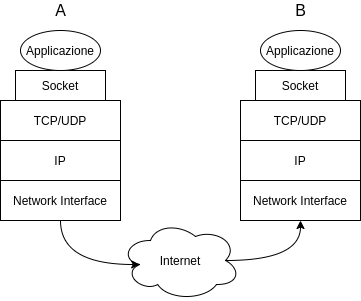
\includegraphics[width=250px]{images/2_Applicazioni_di_rete/socket.png}
\end{figure}

Queste API ci permettono di scegliere quale protocollo di trasporto usare e di configurare alcuni altri piccoli parametri ma di tutto il resto non dovremo preoccuparci minimamente.

\subsubsection{Come scegliere il protocollo di trasporto?}
Le API ci mettono a disposizione 2 protocolli di livello trasporto tra i quali scegliere.
La scelta va ovviamente fatta ponderando le caratteristiche della applicazione, in particolare:
\begin{itemize}
    \item \emph{reliability} - affidabilità: alcune applicazioni tollerano la perdita di informazioni o che l'arrivo delle informazioni non sia nello stesso ordine con il quale sono state inviate (streaming audio/video), per altre applicazioni è importante che i dati arrivino tutti e nell'ordine corretto (file transfer, chat)

    \item \emph{timing} - tempestività: alcune applicazioni hanno necessità che i dati arrivino in maniera veloce (VoIP, streaming), per altre applicazioni un piccolo delay non è importante
    
    \item \emph{throughput}: alcune applicazioni necessitano la garanzia di un minimo di velocità della rete (streaming in diverse qualità), per altri la velocità non è importante (file transfer, email)
    
    \item \emph{security}: per alcune applicazioni sono importanti gli aspetti della sicurezza, dell'integrità dei dati e della loro autenticità, per altre meno
\end{itemize}
I protocolli tra i quali scegliere sono:
\begin{table}[H]
    \centering
    \begin{tabular}{p{150px}|p{150px}}
        \multicolumn{1}{c}{\textbf{TCP}} & 
        \multicolumn{1}{c}{\textbf{UDP}}\\
        \hline        
        Orientato alla connessione, quindi si esegue un setup iniziale prima di poter trasmettere i dati &
        Non ha meccanismi di connessione \\
        \hline
        E' affidabile & 
        Non è affidabile, i pacchetti possono non arrivare o arrivare corrotti\\
        \hline
        Applica un controllo del flusso in modo da non sovraccaricare il ricevente &
        Nessun meccanismo di controllo del flusso \\       
        \hline
        Applica un controllo della congestione, se nota che la rete si avvicina ad una congestione cala drasticamente il  rate dei pacchetti & 
        Nessun meccanismo di controllo del flusso \\
        \hline
        Non fornisce timing, né security, né un throughput minimo &
        Non fornisce timing, né security, né un throughput minimo \\
        \hline
        Spesso chiamato \emph{stream} perché i pacchetti sono correlati l'uno con l'altro &
        Chiamato \emph{datagram} perché ogni pacchetto è da intendere singolarmente, spesso chiamato anche \emph{best effort} \\
    \end{tabular}
\end{table}

\subsection{Definizione di un protocollo applicativo}
Per definire un protocollo applicativo è necessario definire:
\begin{itemize}
    \item Il tipo dei messaggi scambiati: le richieste e le risposte
    \item La sintassi dei singoli messaggi: i campi di cui si compongono, come sono delineati
    \item La semantica del messaggio: il significato dei singoli campi, come vanno letti
    \item Le regole su quando e come i processi inviano e rispondono ai messaggi
\end{itemize}

Alcune di queste specifiche sono di dominio pubblico attraverso i documenti \emph{RFC}, questo si fa per permettere l'interoperabilità attraverso diverse macchine e diversi sistemi operativi. Alcuni di questi sono anche approvati in maniera ufficiale come HTTP e SMTP, altri sono solo definiti ma senza approvazione come BitTorrent.
Altri protocolli invece sono proprietari e quindi non hanno una documentazione ufficiale, ad esempio Skype.

\subsection{Indirizzamento dei processi}
Abbiamo detto che in una rete l'host è identificato da un indirizzo numerico a 32 bit detto indirizzo IP, ogni host può tuttavia eseguire diversi processi, serve quindi un metodo per indirizzarli singolarmente attraverso la rete.
Questo è possibile attraverso un altro numero di 16 bit detto \emph{numero di porta}.
Si dice quindi che un processo è in ascolto su una porta.

\subsection{HTTP}
Il protocollo HTTP è quello utilizzato per navigare il web.
Una pagina web consiste in vari oggetti che possono essere semplici pagine HTML, immagini JPEG, file audio e molto altro.
Quando si contatta un web server si scarica sempre una pagina web che poi ha le indicazioni per arrivare a tanti altri oggetti, questi indirizzi sono detti \emph{Uniform Resource Locator - URL}, per esempio: \emph{http://www.someschool.edu/someDept/pic.gif}, si compone di:
\begin{itemize}
    \item hostname: www.someschool.edu
    \item pathname: someDept/pic.gif
\end{itemize}

E' un protocollo client-server in cui il client è costituito dal browser che richiede e renderizza gli oggetti scaricati mentre il server accoglie le richieste ed invia le risorse richieste.
Usa TCP come protocollo di trasporto, di default usa la porta 80 e sfrutta i messaggi HTTP per formare le richieste.

E' un protocollo \emph{stateless} quindi ogni richiesta è a se stante ed il server da solo non è capace di correlare le diverse richieste l'una con l'altra: questo è comodo in quanto il protocollo è più semplice da implementare, non ci sono politiche di \emph{riconciliazione} dello stato qualora uno dei due dovesse essere corrotto e si limita l'uso della memoria.

\subsubsection{Persistent mode}
HTTP può essere:
\begin{itemize}
    \item Non persistente: viene scambiato al massimo un oggetto per connessione TCP
    \item Persistente: sono permessi più scambi di oggetti sulla stessa connessione TCP
\end{itemize}
E' chiaro che la versione persistente permette di diminuire le attese e l' uso della rete in quanto si risparmiano tutti i pacchetti necessari per instanziare la connessione TCP e per terminarla.

\subsubsection{Formato del messaggio}

La struttura di un messaggio di richiesta è il seguente:
\begin{figure}[H]
    \centering
    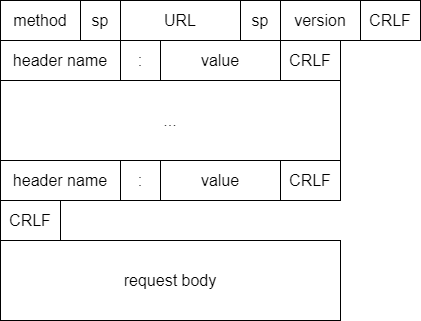
\includegraphics[width=300px]{images/2_Applicazioni_di_rete/HTTP_request.png}
\end{figure}
per esempio:
\begin{verbatim}
    GET /somedir/page.html HTTP/1.1
    Host: www.someschool.edu
    User-Agent: Firefox/15.0
    Connection: close
    Accept-language: it
\end{verbatim}

I metodi fondamentali messi a disposizione sono:
\begin{itemize}
    \item GET: usato dal client per richiedere le risorse
    \item POST: usato dal client per inviare dati, permette di inserire dati nel body
\end{itemize}

Un esempio di risposta è:
\begin{verbatim}
    HTTP/1.1 200 OK
    Connection close
    Date: Wed, 06 Aug 2013 12:00:15 GMT
    Server: Apache/1.3.0 (Unix)
    Last-Modified: Sun, 22 Jun 2013
    Content-Length: 6821
    Content-Type: text/html
    
    data ...
\end{verbatim}

Il protocollo permette di trasmettere eventuali errori tramite gli status header, la prima riga della risposta, composto da un numero (200) e dal significato canonico (OK).

Alcuni RFC che descrivono il protocollo sono:
\begin{itemize}
    \item \href{https://datatracker.ietf.org/doc/html/rfc1945}{1945}
    \item \href{https://datatracker.ietf.org/doc/html/rfc2068}{2068}
    \item \href{https://datatracker.ietf.org/doc/html/rfc2616}{2616}
    \item \href{https://datatracker.ietf.org/doc/html/rfc7230}{7540}
\end{itemize}

\subsubsection{Cookies}
Sono un metodo per rendere stateful il protocollo HTTP.
Quasi tutti i siti usano i cookies per mantenere informazioni attraverso le varie richieste.
Il meccanismo si compone di 4 componenti:
\begin{itemize}
    \item header cookie nella risposta
    \item header cookie nella richiesta
    \item file sul client che mantiene i cookie in memoria
    \item database del sito web che mantiene i dati associati al cookie
\end{itemize}
Il meccanismo funziona in questo modo:
\begin{itemize}
    \item il client esegue una normale richiesta
    \item il server risponde alla richiesta aggiungendo un header Set-Cookie con il nome del cookie, il valore ed altre informazioni utili
    \item alle prossime richieste il client provvederà ad inviare i cookie verso il server come "autenticazione"
    \item il server risponderà con normali risposte
\end{itemize}
All' interno dei cookie l' applicazione può memorizzare:
\begin{itemize}
    \item informazioni utili all' autenticazione
    \item scelta della policy dei cookies
    \item lingua scelta
    \item token della sessione
\end{itemize}

\subsubsection{Web cache - Proxy}
Se visitiamo spesso gli stessi siti è inutile contattare il server ogni volta, magari il server è anche lontano e quindi bisogna fare molta strada per contattarlo.
Per risolvere questo problema ed ottenere un miglioramento generale possiamo pensare di inserire un server nel mezzo tra il client ed il server ed utilizzarlo come una cache.

Una cache è una copia di un dato più vicino al computer e quindi più velocemente contattabile.
Un cache server si comporta sia da client (quando scarica la pagina dal server vero), sia da server (quando lo contattiamo per ottenere i dati copiati).
E' solitamente installata dagli ISP per ridurre il traffico nella rete.

\begin{figure}[H]
    \centering
    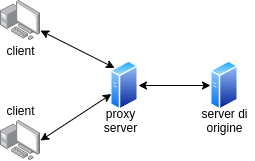
\includegraphics[width=220px]{images/2_Applicazioni_di_rete/cache_example.png}
\end{figure}
Il primo client richiede una risorsa, il proxy server se la procura, quando il secondo client chiede la stessa risorsa il proxy ce l' ha già e gliela fornisce direttamente.

La copia in cache potrebbe tuttavia essere vecchia, per risolvere questo problema è stato introdotto il \emph{conditional GET}, quando il proxy riceve una richiesta contatta il server di origine facendo una normale richiesta ed aggiungendo l'header:
\begin{verbatim}
    If-modified-since: <date>
\end{verbatim}
se il server vede che l' oggetto non è cambiato dalla data comunicata risponde con:
\begin{verbatim}
    HTTP/1.0 304 Not Modified
\end{verbatim}
se invece l' oggetto è stato cambiato si ottiene:
\begin{verbatim}
    HTTP/1.0 200 OK
    <data>
\end{verbatim}
con, appunto, la nuova copia dell' oggetto richiesto.


\subsection{FTP}
FTP sta per File Transfer Protocol, era un protocollo largamente utilizzato per lo scambio di file prima che HTTP esistesse.
E' ancora utilizzato per alcuni tipi di trasferimento come ad esempio per la gestione di spazi web o condivisione di file anonimi.
E' un protocollo client/server che permette di caricare file e scaricare file, quindi scambiare file in entrambe le direzioni.

Usa di default la porta 21 ed è specificato nell' RFC 959.
L' alternativa moderna è quella di utilizzare SFTP che è una versione di FTP che gira sulla porta 22 e prevede il traffico criptato.

Si basa su TCP per avere affidabilità ed una volta avviata la connessione ci si autentica con username e password.
Questa prima connessione sulla porta 21 è detta \emph{di controllo}, permette alcuni comandi come:
\begin{itemize}
    \item ls: elenca i file presenti nella cartella corrente
    \item cd: permette di cambiare la cartella di lavoro
    \item get: permette di scaricare un file
    \item put: permette di caricare un file
\end{itemize}

Usando i comandi get e put il server apre una connessione sulla porta 20, una volta connessi su quella porta possiamo avviare lo scambio del file.
Questa seconda connessione è detta \emph{dei dati}.
Alla fine del trasferimento si chiude questa seconda connessione.
La connessione di controllo rimane aperta per tutto il tempo e può anzi essere utilizzata per inviare altri comandi.

Possiamo quindi dire che:
\begin{itemize}
    \item la connessione di controllo è persitente
    \item la connessione dei dati non è persistente
\end{itemize}

Abbiamo due connessioni diverse perché se facessi tutto con la stessa connessione non potrei lanciare altri comandi nel frattempo.

La connessione di controllo è \emph{out of band} proprio per questa separazione dei canali.

FTP è stateful perché mantiene la directory corrente una volta effettuata l' autenticazione ed anche i file caricati continuano a rimanere sul server per la prossima connessione.

\subsection{Posta elettronica}
La posta elettronica è uno dei primi utilizzi di internet sin dalla nascita, si basa su 2 componenti principali:
\begin{itemize}
    \item \emph{user agent}: programma client usato per inviare e ricevere le mail, alcuni esempi sono elm, Mozilla Thunderbird, ecc.
    
    \item \emph{mail server}: programma server che mantiene in memoria la \emph{mailbox} dell' utente, cioè il contenitore dei messaggi in ingresso e la \emph{coda messaggi} cioè i messaggi in uscita.
    Si basa sul protocollo SMTP che si occupa di eseguire lo scambio delle email tra i diversi server mail.
    Ogni mail server che dialoga tramite SMTP è sia client, quando inizia la connesione per inviare la nuova mail, che server, quando riceve la connessione per ricevere le mail.
\end{itemize}

\subsubsection{SMTP - Simple Mail Transfer Protocol}
Il protocollo SMTP usa TCP per avere uno scambio affidabile, usa di default la porta 25 ed è testuale.
Supponiamo che lo user agent carichi direttamente la mail sul proprio mail server, ora questa mail deve arrivare al mail server del destinatario.
Il mail server guarda il destinatario e trova il mail server associato, inizia una connessione TCP, esegue l' handshake, tramite le regole del protocollo provvede ad inviare la mail e poi esegue una chiusura.
Il server mail al quale ci si connette risponde tramite degli status code e delle frasi, un po' come HTTP.
\begin{verbatim}
    S: 220 hamburger.edu
    C: HELO crepes.fr
    S: 250 Hello crepes.fr, pleased to meet you
    C: MAIL FROM: <alice@crepes.fr>
    S: 250 alice@crepes.fr... Sender ok
    C: RCPT TO: <bob@hamburger.edu>
    S: 250 bob@hamburger.edu ... Recipient ok
    C: DATA
    S: 354 Enter mail, end with "." on a line by itself
    C: Do you like ketchup?
    C: How about pickles?
    C: .
    S: 250 Message accepted for delivery
    C: QUIT
    S: 221 hamburger.edu closing connection
\end{verbatim}

SMTP usa connessioni persistenti, come HTTP, tuttavia SMTP è più un protocollo push in quanto si occupa prettamente di caricare dei dati mentre HTTP è principalmente pull in quanto sono più i download che gli upload.
SMTP usa CRLF.CRLF come terminatore di un messaggio ed invia più oggetti attraverso messaggi multipart cioè spezzettati in diversi pacchetti.

Il formato di un messaggio è:
\begin{figure}[H]
    \centering
    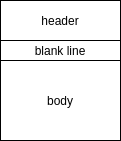
\includegraphics[width=80px]{images/2_Applicazioni_di_rete/messaggio_smtp.png}
\end{figure}
Alcuni esempi di header sono:
\begin{itemize}
    \item To
    \item From
    \item Subject
\end{itemize}
che sono diversi dai comandi SMTP!

Il body invece contiene il messaggio in soli caratteri ASCII.

Sappiamo che alle email possiamo aggiungere degli allegati non per forza testuali ma il protocollo ammette solo un body testuale.
Per avere questa feature altri due RFC sono stati creati: 2045 e 2046.
Questi documenti definiscono l'uso del MIME - Multipurpose Internet Mail Extensions, si tratta di due header aggiuntivi:
\begin{itemize}
    \item Content-Transfer-Encoding: specifica la codifica utilizzata per inviare il file (es: base64)
    \item Content-Type: specifica il tipo di file che si sta inviando, è utile per permettere a chi riceve di eseguire varie azioni in base al tipo
\end{itemize}

\subsubsection{POP3 - IMAP - WebMail}
Lo user agent deve connettersi al mail server corrispondente per scaricare le inbox ed inviare i messaggi in uscita.
Il protocollo POP3 - Post Office Protocol inizia con una autenticazione e poi usa la modalità \emph{download-and-keep}, POP3 è stateless tra le varie sessioni.
IMAP - Internet Mail Access Protocol è molto simile a POP3 ma ha più feature, anche lui tiene i messaggi sul server senza cancellarli, permette anche di organizzare le email in cartelle, è stateful attraverso le sessioni in quanto mantiene un mapping tra i messaggi e le cartelle assegnate.

In fine c'è la Webmail, lo user agent è un browser e le email vengono inviate attraverso HTTP.

\subsection{DNS}
Ricordare gli indirizzi IP, seppure in notazione decimale puntata, è difficile alla lunga, ci viene molto più comodo memorizzare dei nomi.
Proprio per questo motivo esistono gli \emph{hostname} cioè dei nomi associati ad uno o più indirizzi IP.
La traduzione da un nome all'indirizzo associato è detta \emph{risoluzione} e di questo compito si occupa il protocollo DNS.

E' un protocollo applicativo basato su UDP per avere una forte responsività, usa la porta 53 di default.
Per registrare un proprio dominio ci si rivolge ad un \emph{registrar} e dietro compenso lui si occupa di aggiungere i record DNS necessari.
Il DNS fornisce anche altri servizi:
\begin{itemize}
    \item traduzione da hostname ad indirizzo IP

    \item host aliasing: traduzione da un hostname ad un altro detto \emph{canonico}.
    Es: www.iet.unipi.it $\xrightarrow{}$ info.iet.unipi.it

    \item mail server aliasing: traduce gli indirizzi email negli hostname dei server associati a quell' indirizzo.
    Es: bob@hotmail.com $\xrightarrow{}$ server-1.hotmail.com

    \item distribuzione del carico: in base alle richieste ottenute posso tradurre un hostname con un indirizzo IP o con un altro in modo da usare equamente tutti i mirror di un servizio.
    Per fare ciò il server DNS restituisce l'intero elenco di IP associati al dominio ma ogni volta ruota la lista in modo da farne comparire in alto uno diverso.
\end{itemize}

Per dare un ordine ed evitare che lo stesso hostname sia modificato da più enti diversi il DNS fa uso di un database \emph{gerarchico} e \emph{distribuito}.
Distribuito per evitare un single point of failure; un singolo server sovraccaricato di richieste, magari anche distante per alcuni host, in pratica non è facilmente \emph{scalabile}.

\subsubsection{Prima approssimazione}
Un client vuole risolvere www.amazon.com, esegue una query DNS al \emph{root server} per trovare il DNS server che si occupa dei domini .com.
Successivamente il client esegue una query su quel DNS per ottenere l' indirizzo del DNS server associato al dominio amazon.com.
In fine il client contatta questo ultimo server DNS per ottenere l' IP di www.amazon.com

I root name server sono 13 in tutto il mondo, ognuno dei quali poi è ridondato tramite altri mirror, questa distribuzione fa si che in media il tempo per contattare questi DNS sia uguale dappertutto (per guardare i root nameserver consultare \href{https://www.root-servers.org/}{www.root-servers.org}).

\subsubsection{TLD server}
Sono i server Top-Level-Domain cioè i server che si occupano di gestire tutti i domini che finiscono in .com, .org, .net e tutti i top level domain dei vari paesi come .it, .uk, .fr, ecc.

\subsubsection{Authoritative server}
Sono quei server DNS che si occupano di risolvere tutti i sottodomini sotto un dominio, in genere sono tenuti da organizzazioni e service provider.
Sono utili in una azienda per gestire i domini interni come mail, web, ecc.

\subsubsection{Local DNS server}
E' il server al quale gli host si rivolgono nella realtà, esegue la vera e propria traduzione contattando i diversi DNS server necessari e restituisce il risultato all' host che ha eseguito la query.
Solitamente è mantenuto dall' ISP ed agisce come un proxy implementando anche una cache.

\subsubsection{Risoluzione iterativa}
\begin{figure}[H]
    \centering
    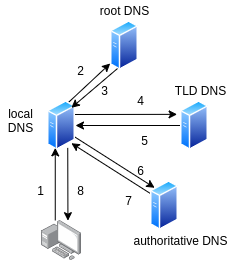
\includegraphics[width=200px]{images/2_Applicazioni_di_rete/risoluzione_DNS.png}
\end{figure}
Supponiamo che l' host richieda la risoluzione di www.unipi.it: esegue la sua query verso il suo local DNS, il local DNS contatta prima il root DNS per ottenere l' indirizzo IP del TLD DNS responsabile di .it, una volta avuto il suo indirizzo lo interroga per ottenere l' IP dell'authoritative DNS di unipi.it, in fine a lui chiede la risoluzione di www.unipi.it.

\subsubsection{Risoluzione ricorsiva}
\begin{figure}[H]
    \centering
    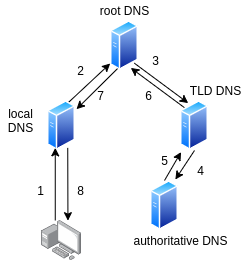
\includegraphics[width=200px]{images/2_Applicazioni_di_rete/risoluzione_DNS_ricorsiva.png}
\end{figure}
In questa configurazione ogni server contattato si occupa di risolvere interamente la query richiesta.
Tuttavia aumenta il carico sui server interemedi che generalmente sarebbero più liberi.

\subsubsection{Caching}
Ogni DNS server ha la propria cache, anche l' host stesso, il timeout delle entries è di solito 2 giorni.

In particolare i TLD DNS server sono cachati nel local DNS perché sono tante le richieste per lo stesso TLD.

\subsubsection{Record DNS}
La struttura di un record DNS è:
$$ (name, value, type, ttl) $$
il ttl è il Time-To-Live cioè il tempo per il quale il record è valido.
Esistono vari tipi di record DNS, i più comuni sono:
\begin{itemize}
    \item tipo A: name contiene l' hostname, value contiene l' IP

    \item tipo CNAME: name contiene l' alias per qualche nome, mentre value contiene il nome canonico

    Es: (www.hal.com, servereast.backup2.hal.com)

    \item tipo NS: name contiene il dominio, value contiene l' hostname dell' authoritative DNS per quel dominio
    
    Es: (hal.com, dns.hal.com)
    
    \item tipo MX (mail exchange): name contiene il dominio, value contiene il nome canonico del mailserver associato al dominio
\end{itemize}

\subsection{Distribuzione di file - comparazione tra C/S e p2p}
Quanto tempo serve per distribuire un file da 1 server ad N peer?
\begin{figure}[H]
    \centering
    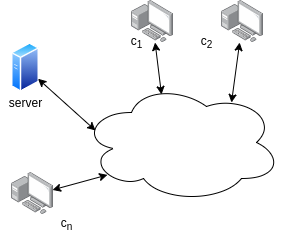
\includegraphics[width=220px]{images/2_Applicazioni_di_rete/distribuzione_file.png}
\end{figure}
Poniamo i seguenti dati:
\begin{itemize}
    \item $F$: dimensione del file
    \item $u_s$: velocità di upload del server
    \item $u_i$: velocità di upload del peer $i$
    \item $d_i$: velocità di download del peer $i$
\end{itemize}
Usando un' architettura client/server la velocità per scaricare un file può essere:
\begin{itemize}
    \item $\frac{NF}{u_s}$: tempo che serve al server per inviare il file a tutti
    \item $\frac{F}{d_i}$: tempo necessario al client per ricevere il file
\end{itemize}
In definitiva abbiamo:
$$ d_{cs} = max\{ \frac{NF}{u_s}, \frac{F}{d_i} \} $$
per $N \xrightarrow{} \infty$ il termine cresce in maniera lineare.

Usando un' architettura p2p la velocità per scaricare un file può essere:
\begin{itemize}
    \item $\frac{F}{u_s}$: prima copia
    \item $\frac{F}{min\{d_i\}_i}$: tempo per caricare il file nel nodo con velocità minore
    \item $\frac{NF}{\left( u_s + \sum u_i \right)}$: tempo per scaricare $N$ copie del file usado il massimo upload rate
\end{itemize}
Si noti che il terzo termine ha il denominatore che può essere assunto come $\left( u_s + Nu_{medio}\right)$ quindi:
$$ \frac{NF}{u_s + Nu_{medio}} \xrightarrow{N \xrightarrow{} \infty} \frac{F}{u_{medio}} $$
\begin{figure}[H]
    \centering
    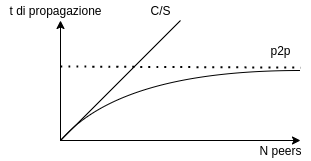
\includegraphics[width=200px]{images/2_Applicazioni_di_rete/comparazione_cs_p2p.png}
\end{figure}

\subsection{Ricerca di informazioni in una rete p2p}
Essendo una rete distribuita è necessario sapere dove trovare le risorse che si cercano.
Se un peer mette a disposizione dei file, un altro peer deve poter cercare e sapere cosa ha a disposizione.
Se parliamo di un protocollo di messaging invece è necessario conoscere l' IP accoppiato ad un username in modo da effettuare la connessione diretta.
Ci serve pertanto un indice nel quale effettuare le nostre query di ricerca.
Supponiamo quindi di dover creare un database i cui record sono formati da: (chiave, valore) in cui la chiave è il contenuto che vogliamo cercare ed il valore è l' IP del nodo che la possiede.
I peer dovranno poter eseguire query in questo database ed anche inserire delle entry in modo che possano essere utili agli altri.
Vediamo alcuni approcci.

\subsubsection{Centralized Index}
Il servizio di indicizzazione è offerto da uno o più server centralizzati, quando un nodo torna online lo notifica al server che provvede ad aggiornare il suo database, quando si esegue una query si contatta il server che risponde alla richiesta.
Siamo davanti ad un approccio ibrido in quanto l'indicizzazione e quindi la ricerca dei contenuti è client/server mentre lo scambio dei file o dei messaggi è p2p in quanto avviene tramite connessione diretta dei peer.

Un esempio di questa struttura è quella offerta da Napster che permetteva di cercare la musica presente nella rete p2p tramite il suo server centralizzato, ma poi il vero e proprio scambio avveniva in modalità p2p.

Questo approccio ha alcuni problemi:
\begin{itemize}
    \item costituisce un single point of failure, come qualsiasi servizio centralizzato
    \item potrebbe portare a problemi di performance in quanto tutte le richieste sono fatte allo stesso host
    \item la responsabilità del servizio in caso di problemi legali può essere attribuita a chi mantiene il server di indicizzazione
\end{itemize}

\begin{figure}[H]
    \centering
    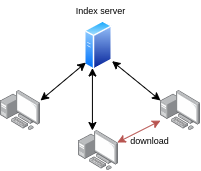
\includegraphics[width=200px]{images/2_Applicazioni_di_rete/centralized_index.png}
\end{figure}

\subsubsection{Query flooding}
E' un approccio completamente decentralizzato, usato dall' originale GNUtella.
L' indice è distribuito su tutti i nodi della rete che distribuiscono contenuti, i nodi sono connessi tra di loro a formare un gigantesco grafo.
Quando si deve eseguire una query di ricerca si forgia una richiesta e la si invia a tutti i propri nodi adiacenti: se loro hanno la richiesta risponderanno, altrimenti propagheranno la richiesta ai loro adiacenti e così via.
Si parla di \emph{flooding} proprio perché il numero di richieste che circola all' interno della rete è grandissimo. Se la rete diventa molto grande per problemi di scalabilità si può passare ad eseguire delle \emph{limited-scope query}: la propagazione viene eseguita un numero massimo di volte, per esempio dopo il terzo hop la richiesta non si ripete più.
Questo tuttavia può portare a dei falsi negativi: non troviamo la risorsa non perché non ci sia ma perché non siamo arrivati all' host che la fornisce.

\begin{figure}[H]
    \centering
    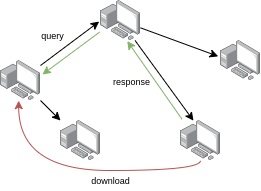
\includegraphics[width=250px]{images/2_Applicazioni_di_rete/query_flooding.png}
\end{figure}

Per costruire una rete del genere il protocollo GNUtella si serve di una lista di peer molto attivi, oppure di un server tracker che registra un insieme di IP di peer.
Quando un nuovo nodo vuole entrare a far parte della rete usa una di queste liste per ottenere alcuni IP di altri nodi, inizia dunque una connessione TCP ed invia un messaggio \emph{ping} con un campo \emph{peer-count} inizializzato ad un certo valore, ogni nodo che riceve questo ping lo ritrasmette ai suoi vicini decrementando peer-count fino ad arrivare a 0.
Qualsiasi host riceva questo ping risponde con un \emph{pong} in cui inserisce anche il proprio IP per permettere la connessione TCP.

\subsubsection{Hierarchical overlay}
E' una via di mezzo tra i due precedenti, utilizza dei nodi più importanti degli altri detti \emph{supernodi} per slegarsi da una centralizzazione ma non allarga troppo la lista dei peer che costruiscono l' indice.
Questi supernodi sono nodi con alta banda, con lunghi tempi online, sono connessi tra di loro a formare una seconda rete ed ognungo di loro contiene una porzione dell' indice che propaga agli altri.
I peer normali si connettono ai supernodi per informarli del loro contenuto e per eseguire le query di ricerca, una volta ottenuto il record di risposta si provvede ad una normale connessione p2p.

\begin{figure}[H]
    \centering
    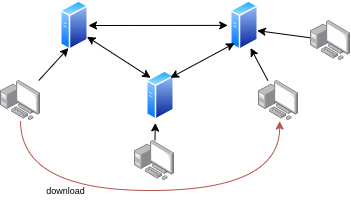
\includegraphics[width=280px]{images/2_Applicazioni_di_rete/hierarchical_overlay.png}
\end{figure}

\subsubsection{Distributed hash table}
E' un database p2p distribuito, usato da eMule.
Si assegna un identificatore di peer nel range [0, $2^{n-1}$], e le chiavi utilizzate sono nello stesso range.
Le chiavi sono ottenute passando la chiave di ricerca all' interno di una funzione di hash.
Le tuple (chiave, valore) sono associate ai peer in modo che ogni chiave sia associata al peer con l'ID più vicino ma maggiore, questo peer è chiamato \emph{successore immediato}.

Es: se $n = 4$ ed abbiamo i peer: [1, 3, 4, 5, 8, 10, 12, 14], la chiave 13 ha come immediato successore 14, la chiave 15 ha come immediato successore 1, ecc.

Ogni peer è a conoscenza solo del suo immediato successore e del suo predecessore, abbiamo di fatto una lista circolare.
Quando un nodo deve aggiungere un nuovo record o cercare tramite la chiave invia la richiesta al suo immediato successore e così via finché la tupla non raggiunge l' host con ID più vicino e maggiore, a quel punto il responsabile per quella chiave risponde direttamente tramite l' IP all' interno della richiesta.

Questa struttura impiega complessità $O(N)$ per eseguire una query, possiamo abbreviarla inserendo delle shortcut e permettendo quindi connessioni anche oltre all' immediato successore.
Si può quindi passare ad avere ogni nodo connesso a $O(logN)$ vicini, facendo scendere anche la complessità della richiesta a $O(logN)$.

Per gestire la scomparsa di un host dalla rete ogni peer oltre a conoscere il suo successivo conosce anche il successivo del successivo, periodicamente pinga i due successivi e se qualcuno è andato offline provvede a riconfigurare la sua posizione nell' anello.

\begin{figure}[H]
    \centering
    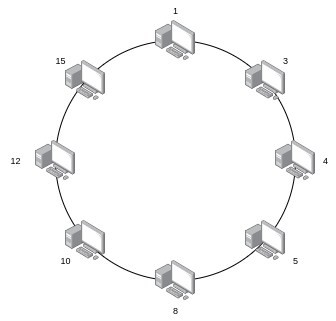
\includegraphics[width=200px]{images/2_Applicazioni_di_rete/DHT.png}
\end{figure}

\subsubsection{BitTorrent}
E' un protocollo di scambio di file che permette di scaricare da più peer contemporaneamente:
\begin{figure}[H]
    \centering
    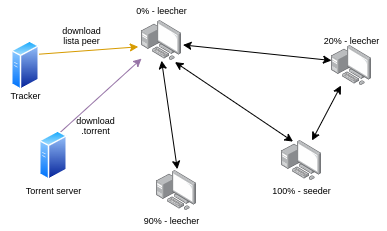
\includegraphics[width=250px]{images/2_Applicazioni_di_rete/bittorrent.png}
\end{figure}
I file da scambiare sono divisi in chunk da 256KB.
Ogni nodo della rete è un peer, ma può svolgere compiti diversi:
\begin{itemize}
    \item torrent server: è un server, spesso non facente parte della vera rete di distribuzione dei chunk, che mantiene in memoria i file .torrent e permette a chiunque di scaricarli.

    \item tracker: è un server che traccia i peer che fanno parte della rete di distribuzione di un torrent in modo da metterli in contatto tra di loro
    
    \item seeder: peer che ha completamente scaricato i file puntati dal torrent e continua a distribuirli
    
    \item leecher: peer che non ha ancora completato il download dei file, scarica i nuovi chunk ed allo stesso tempo carica i chunk che possiede
\end{itemize}

I file .torrent sono file che contengono informazioni sulla rete, in particolare l' IP del tracker e le informazioni sui chunk da cercare (hash dei blocchi in modo da non poterli sostituire arbitrariamente).

Quando si vuole entrare nella rete si contatta il tracker e si inizia una connessione con i peer inviati come risposta dal tracker.
Il trasferimento avviene in chunk quindi ad ogni istante ogni peer ha un certo numero di chunk.
Quando ci si connette agli altri peer, ed anche ad intervalli regolari, ci si scambia la lista dei chunk posseduti da ognuno in modo da decidere quale altro richiedere.
Quando si richiede non importa l' ordine perché tanto poi possono essere riordinati a posteriori, tuttavia si usa la metrica del \emph{rarest first}, cioè una volta chiesta la lista alle proprie connessioni si richiedono prima i chunk meno comuni, questo si fa per aumentare la presenza di questi chunk nella rete.

La scelta delle proprie connessioni è eseguita tramite la logica \emph{tit-for-tat} cioè si hanno 4 connessioni contemporaneamente con i 4 peer con il più alto rate di trasmissione.
Ogni 10 secondi si rivaluta questo gruppo ed ogni 30 secondi si sceglie casualmente un altro peer per iniziare a scambiare chunk. Questo per verificare se sia conveniente modificare i 4 migliori in questo momento: \emph{optimistically unchoke}.

\subsubsection{Skype}
Skype è un protocollo proprietario di messaggistica.
Ha una architettura a supernodi e l' indice mappa gli username agli IP.
Se i nodi sono dietro NAT per comunicare si usano i supernodi come relay per trasmettere il traffico.
E' un esempio di applicazione real-time.

\subsection{Socket}
Sono una interfaccia inizialmente costruita per BSD4.1 UNIX, nel 1981, usata per creare applicazioni di rete.
Sono strutture esplicitamente create, usate e rilasciate dalle applicazioni tramite chiamate a sistema.
Sfruttano un paradigma client/server ma sono abbastanza flessibili da poter creare anche applicazioni p2p.

Permettono di utilizzare 2 protocolli di trasporto:
\begin{itemize}
    \item quello a datagramma: UDP
    \item quello a stream: TCP
\end{itemize}
Dallo stesso socket una applicazione può ricevere ed inviare messaggi.
Oltre che attraverso la rete possono essere usati anche per inter-process comunication tra processi sulla stessa macchina.

Un socket è identificato da un indirizzo IP, quello della macchina che lo ha aperto, e da una porta, un numero identificativo richiesto dal programma stesso che gestisce il socket.
Per comunicare si usano due socket, uno per ogni endpoint della comunicazione.

\section{Reti a connessione diretta - Data Link Layer}
Abbiamo dei nodi connessi tra di loro attraverso dei link di connessione, ne possiamo avere di diverso tipo: cavi elettrici, fibre ottiche, connessioni via etere, ecc.
Ci serve per tanto dell' hardware che permetta di codificare i bit che vogliamo trasmettere in un segnale elettrico/luminoso/elettromagnetico in modo da poter essere trasportato dal link fisico.
Questa codifica (\emph{encoding}) è eseguita da un trasmettitore, all' altro capo del link vi deve essere invece un ricevitore che effettui la decodifica (\emph{decoding}).
Una semplice codifica che possiamo immaginare attraverso un link in rame può essere:
\begin{itemize}
    \item livello alto di tensione: 1 logico
    \item livello basso di tensione: 0 logico
\end{itemize}
\begin{figure}[H]
    \centering
    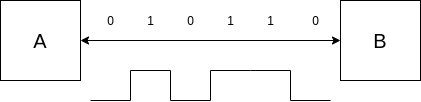
\includegraphics[width=300px]{images/3_Reti_connessione_diretta/encoding.png}
\end{figure}
tuttavia ce ne possono essere diverse in base al mezzo, alla velocità da usare, ecc, ma sono tutte questioni che riguardano la teoria dei segnali e non le reti in se per se.

Essendo la trasmissione bidirezionale ogni capo della connessione è dotato di un trasmettitore ed un ricevitore, lo chiamiamo ricetrasmettitore (\emph{transceiver}).

Ovviamente il canale di trasmissione non è ideale, il che comporta problemi di attenuazione (il segnale perde di potenza durante il percorso), disturbi, rumore ed altro che possono portare il segnale a cambiare in maniera importante, modificando quindi il contenuto delle informazioni che trasporta.

Anche la campionatura del segnale è problematica: per campionare al meglio sarebbe necessario campionare sul picco, ma non abbiamo la certezza di quando il picco avvenga.
Se i due endpoint non sono sincronizzati un capo non sa quando è il picco dell' altro capo, anche se fossero sincronizzati i circuiti del clock non sono perfettamente identici quindi il drift li porterebbe fuori sincro in poco tempo.

E' utile definire l' error rate:
$$ \text{error\_rate} = \frac{\text{bit\_errati}}{\text{bit\_trasmessi}} $$

Il Data Link Layer è il layer dello stack ISO/OSI che si occupa di fornire l' astrazione di un canale affidabile.
Non importa cosa c' è al livello fisico, l' importante è che i dati vengano trasmessi bene tra due endpoint connessi in maniera diretta.



\subsection{Servizi del data-link layer}
Per ottenere l' affidabilità il data-link layer porta avanti alcune politiche.

\subsubsection{Framing}
Dato un error\_rate piccolo a piacere, se trasmetto tanti bit avrò sempre qualche bit che non arriva a destinazione in maniera corretta.
Per risolvere possiamo dividere il datagramma intero in dei \emph{frame} più piccoli ed aggiungervi un \emph{header} ed un \emph{trailer}.
\begin{figure}[H]
    \centering
    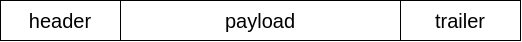
\includegraphics[width=250px]{images/3_Reti_connessione_diretta/frame.png}
\end{figure}

\subsubsection{Error detection \& correction}
Si occupa di capire se ci sono degli errori ed eventualmente correggerli.
Si applicano alcuni algoritmi che permettono di dire quale bit è arrivato in maniera errata e quindi flipparlo.
Questi algoritmi tuttavia sono affidabili solo per pochi bit errati ed a volte sono troppo pesanti in termini di bit aggiuntivi da inserire nel frame.

\subsubsection{Trasmissione dati affidabile}
Un' altra tecnica utilizzata è quella tramite acknowledge e ritrasmissione: quando ho ricevuto un frame lo segnalo, se qualche frame mi manca o è danneggiato lo chiedo nuovamente.
In fine riordino i frame per ottenere il datagramma intero.

\subsubsection{Flow control}
Permette di gestire la velocità con la quale inviare i dati sul media, questo è comodo qualora si interfaccino hardware diversi che non hanno la stessa velocità massima.

\subsubsection{Half-duplex e full-duplex}
Permette di negoziare, tramite il tipo di mezzo, se la connessione deve essere:
\begin{itemize}
    \item half-duplex: comunicazione bidirezionale ma uno per volta
    \item full-duplex: comunicazione bidirezionale e simultanea
\end{itemize}

\subsubsection{Implementazione}
Il data-link layer è implementato principalmente in hardware all' interno della Network Interface Card (NIC) in quanto deve interfacciarsi con il link fisico, tuttavia altre componenti, quelle più ad alto livello possono essere implementate interamente in software.

\subsection{Error detection}
L' algoritmo generico di error detection prevede che il trasmettitore aggiunga ai dati dei bit R ridondanti utilizzati dal ricevitore per controllare che i dati siano arrivati correttamente.
Questi bit R si aggiungono alla fine in modo che siano generati contestualmente alla trasmissione \emph{on-the-fly} ed il controllo possa avvenire durante la ricezione.
Ovviamente durante la trasmissione possono corrompersi sia i bit D che i bit R, supponiamo quindi che il ricevitore ottenga D' ed R': usa lo stesso algoritmo del trasmettitore che a partire dai bit D' genera i bit ridondati, li compara ai bit R' ricevuti ed agisce di conseguenza se sono diversi.

La error detection non è affidabile al 100\%, possono esserci alcuni casi limite dei vari algoritmi che non permettono di rilevare correttamente gli errori.
In genere aumentare il numero di bit R porta ad una migliore detection ma anche ad un maggiore numero di bit, non di dato, da inviare.

\subsubsection{Parity checking}
Si aggiunge in coda al messaggio un singolo bit di parità, questo bit si sceglie in modo da rendere pari il  numero di 1 all' interno del blocco, nella parità pari, oppure per rendere il conteggio dispari, nella parità dispari.
Questo metodo è usato per brevissimi spostamenti, ad esempio quelli memoria-CPU perché è poco affidabile, infatti riesce a rilevare il cambiamento di un singolo bit, ma se ve ne sono due modificati allora il bit di parità è corretto pur non essendolo il campo dati.

In hardware si può implementare tramite lo XOR/XNOR dei bit del campo dati.
\begin{figure}[H]
    \centering
    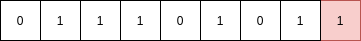
\includegraphics[width=200px]{images/3_Reti_connessione_diretta/parity_checking.png}
\end{figure}

\subsubsection{Checksum}
Si splitta il pacchetto in blocchi da 16 bit, li si tratta come interi e si esegue la somma bit a bit (complemento ad 1) di tutti i gruppi.
Il risultato di questa somma è detto \emph{checksum} e lo aggiungo in coda al pacchetto oppure in un campo ben preciso se il protocollo lo prevede (ad esempo il TCP usa questo algoritmo ed ha un campo del pacchetto apposito).
Il ricevitore ovviamente esegue la stessa somma, controlla con il valore ricevuto, se non matchano c'è la certezza che ci sia stato un errore durante la trasmissione.
Anche in questo caso non si può avere la certezza al 100\% che se i valori matchano allora i dati ricevuti sono corretti.

\subsubsection{Cyclic redundancy check - CRC}
Questo algoritmo è largamente utilizzato all' interno dei vari protocolli di data link (ad esempio Ethernet, 802.11 WiFi, ecc).
Vede il blocco di dati $D$ come un unico numero, si sceglie un numero di $r+1$ bit e lo si chiama $G$ (\emph{generatore}), scelgo opportunamente gli $r$ bit di parità e li chiamo $R$, li scelgo in modo che la concatenazione $<D, R>$ sia divisibile per $G$ nell' aritmetica modulo 2.
Quando il ricevitore riceve il numero prova ad eseguire la divisione per $G$, se il resto non è nullo ci sono stati degli errori nella trasmissione.
Questo algoritmo riesce a trovare i burst di errori con lunghezza minore di $r+1$ bit.

Si noti che il generatore $G$ deve essere comune a tutti e due gli endpoint, per far ciò si può prevedere un valore fisso all' interno del protocollo oppure negoziarne uno alla prima connessione.

Per trovare $R$ opportuno si deve risolvere questa equazione:
$$ D \cdot 2^{r} \oplus R = n \cdot G $$
$$ D \cdot 2^{r} = n \cdot G \oplus R $$
se dividiamo $D \cdot 2^r$ per $G$ il resto è uguale ad $R$:
$$ R = resto\left( \frac{D \cdot 2^r}{G} \right) $$

\subsection{Forward error correction}
Alcuni algoritmi oltre a mostrare che ci sono stati errori permettono di correggerli se sono in un giusto numero.

\subsubsection{Two-dimensional bit parity}
Si aggiungono al messaggio un bit di parità per ogni riga ed uno per ogni colonna ed incrociando i bit di parità sbagliati si trova il bit errato:
\begin{table}[ht!]
    \centering
    \begin{tabular}{c c c | c}
        $d_{1,1}$ & ... & $d_{1,j}$ & $d_{1,j+1}$ \\
        $d_{2,1}$ & ... & $d_{2,j}$ & $d_{2,j+1}$ \\
        ... & ... & ... & ... \\
        $d_{i,1}$ & ... & $d_{i,j}$ & $d_{i,j+1}$ \\
        \hline
        $d_{i+1,1}$ & ... & $d_{i+1,j}$ & $d_{i+1,j+1}$ \\
    \end{tabular}
\end{table}
Questo algoritmo prevede di introdurre quindi $i + j + 1$ bit di parità.

\subsection{Reliable data transfer}
Vogliamo creare l' astrazione di un trasporto dati affidabile: il layer in alto chiama una procedura che si occupa di inviare i dati ed essere certo che siano arrivati in maniera corretta, così come dall' altra parte essere sicuri che i dati ricevuti siano corretti.
Le interfacce che offrono questa astrazione sono:
\begin{itemize}
    \item \emph{rdt\_send}: procedura chiamata dal layer superiore per inviare dati
    \item \emph{deliver\_data}: procedura chiamata dal data link per consegnare i dati al layer superiore
\end{itemize}
Il data-link layer invece sfrutta le seguenti primitive messe a disposizione dal layer fisico:
\begin{itemize}
    \item \emph{udt\_send}: chiamata per inviare un pacchetto di dati su un canale non affidabile
    \item \emph{rdt\_rcv}: chiamata dal layer fisico quando arriva un nuovo pacchetto sul canale
\end{itemize}

Implementiamo un protocollo per affinamenti successivi ed usiamo il formalismo degli automi a stati finiti per descriverne il comportamento.


\subsubsection{RDT 1.0: rdt su un canale affidabile}
Su un canale affidabile non abbiamo errori durante la trasmissione e non abbiamo perdita di pacchetti, la situazione è semplicemente rappresentabile:
\begin{figure}[H]
    \centering
    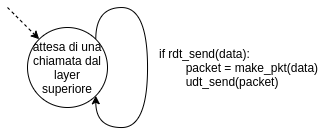
\includegraphics[width=200px]{images/3_Reti_connessione_diretta/rdt_1.0_sender.png}
    \caption{RDT 1.0 sender}
\end{figure}
Siamo sempre in attesa di una chiamata dal layer superiore, quando arriva una chiamata prendiamo i dati, prepariamo il pacchetto e lo spediamo sul canale.

\begin{figure}[H]
    \centering
    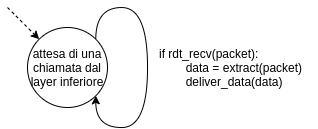
\includegraphics[width=200px]{images/3_Reti_connessione_diretta/rdt_1.0_receiver.png}
    \caption{RDT 1.0 receiver}
\end{figure}
Siamo sempre in attesa di una chiamata dal layer inferiore, quando arriva un pacchetto lo prendiamo, estraiamo i dati che vi sono contenuti all' interno e lo consegnamo al layer superiore.


\subsubsection{RDT 2.0: canale che può flippare i bit}
Introduciamo ora un canale che durante la trasmissione possa flippare alcuni bit presenti nel pacchetto.
Ci serve quindi un meccanismo di error detection (CRC o checksum in base al layer sul quale stiamo lavorando) per capire quando gli errori ci sono stati, ci serve poi anche un metodo per aggiustare la situazione.
Introduciamo quindi i concetti di \emph{acknowledgement} - ACK, con il quale il ricevitore notifica al trasmettitore l' avvenuta ricezione del pacchetto corretto e \emph{negative acknowledgement} - NAK, con il quale il ricevitore notifica al trasmettitore di aver ricevuto il pacchetto corrotto e ne richiede la ritrasmisione.

Stiamo quindi implementando una forma di Automatic Repeat reQuest - ARQ protocol.

\begin{figure}[H]
    \centering
    
\includegraphics[width=300px]{images/3_Reti_connessione_diretta/rdt_2.0_sender.png}
    \caption{RDT 2.0 sender}
\end{figure}
Si attende una chiamata dal layer superiore, quando avviene si costruisce il pacchetto e lo si invia sul canale.
Si rimane quindi in attesa di un feedback, quando arriva se è positivo si torna in attesa di una chiamata dal layer superiore, se è negativo invece si reinvia il pacchetto e si torna in attesa di un feedback.

\begin{figure}[H]
    \centering
    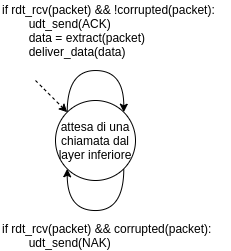
\includegraphics[width=150px]{images/3_Reti_connessione_diretta/rdt_2.0_receiver.png}
    \caption{RDT 2.0 receiver}
\end{figure}
Si attende l' arrivo di un pacchetto, quando arriva si controlla il suo stato, se non risulta corrotto allora si invia un ACK, si estraggono i dati e li si inviano al layer superiore, dopodiché si torna in attesa, se invece risulta corrotto si invia un NAK, si butta via il pacchetto e si ritorna in attesa.

Questo protocollo è basato sulla politica di \emph{stop-and-wait} cioè si invia un pacchetto e si aspetta per una risposta prima di fare qualsiasi cosa, vedremo più avanti che questo approccio è poco furbo in quanto si perde tanto tempo in attesa ma per adesso rimaniamo con questa logica.


\subsubsection{RDT 2.1: gestione degli errori sugli ACK/NAK}
Il protocollo precedente ha una falla importante: non abbiamo la certezza che ACK e NAK vengano trasmessi correttamente, essendo trasferiti sullo stesso canale non affidabile potrebbero arrivare in maniera errata, come potrebbero non arrivare.
Inoltre dato che c'è di mezzo una ritrasmissione c'è da accertarsi che i pacchetti che consegnamo al layer superiore non siano duplicati!
Per gestire i duplicati possiamo aggiungere al pacchetto un numero di sequenza, per protocolli stop-and-wait basta un solo bit di sequenza.
\begin{figure}[H]
    \centering
    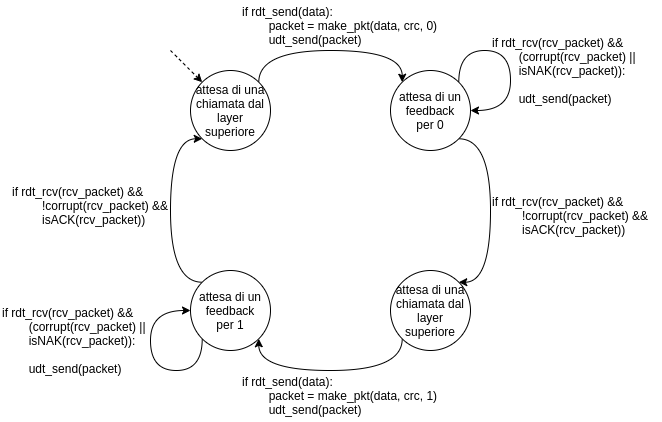
\includegraphics[width=340px]{images/3_Reti_connessione_diretta/rdt_2.1_sender.png}
    \caption{RDT 2.1 sender}
\end{figure}
All' arrivo di una richiesta costruiamo il pacchetto con sequence\_number a 0, lo inviamo, aspettiamo un feedback.
Se il feedback è negativo allora re-inviamo il messaggio, altrimenti ci portiamo in attesa della prossima richiesta.
Quando arriva una seconda richiesta costruiamo un nuovo pacchetto con sequence\_number ad 1, lo inviamo e ci mettiamo in attesa del feedback.
Quando arriva un feedback se è positivo torniamo in attesa di una richiesta, altrimenti rispediamo il pacchetto rimettendoci in attesa del feedback.

\begin{figure}[H]
    \centering
    
\includegraphics[width=340px]{images/3_Reti_connessione_diretta/rdt_2.1_receiver.png}
    \caption{RDT 2.1 receiver}
\end{figure}
All' arrivo di un pacchetto:
\begin{itemize}
    \item se non è corrotto ed ha sequence\_number 0: estraggo i dati e li consegno al layer superiore, invio un ACK e mi metto in attesa di un pacchetto con sequence\_number 1
    \item se è corrotto: invio un NAK
    \item se non è corrotto ma ha sequence\_number 0: invio un ACK e butto via il pacchetto in quanto siamo in caso di duplicati
\end{itemize}
stessa cosa per l' attesa del pacchetto con sequence\_number 1.


\subsubsection{RDT 2.2: protocollo NAK-free}
Possiamo evolvere il protocollo precedente eliminando i NAK ed eseguendo tutto tramite ACK.
Per fare ciò usiamo gli ACK aggiungendo il sequence\_number del pachetto di cui si sta confermando la corretta ricezione.
Il trasmettitore invece quando si vede arrivare un ACK con sequence\_number diverso dall' ultimo inviato re-invia il pacchetto.
\begin{figure}[H]
    \centering
    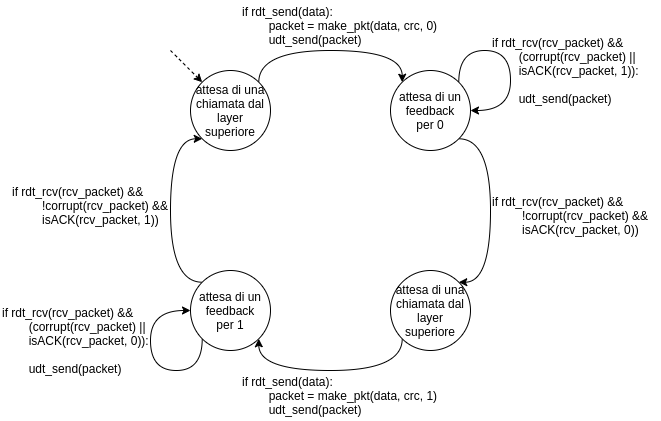
\includegraphics[width=340px]{images/3_Reti_connessione_diretta/rdt_2.2_sender.png}
    \caption{RDT 2.2 sender}
\end{figure}

\begin{figure}[H]
    \centering
    
\includegraphics[width=340px]{images/3_Reti_connessione_diretta/rdt_2.2_receiver.png}
    \caption{RDT 2.2 receiver}
\end{figure}
Il ricevitore è visibilmente semplificato.

\subsubsection{RDT 3.0: canale con errori e perdite di pacchetti}
Su una connessione nella quale posso perdere dei pacchetti la detection degli errori ed il sequence\_number non sono abbastanza per risolvere tutte le problematiche.
Non possiamo accorgerci direttamente della perdita di un pacchetto, quindi come tattica usiamo quella dell' attesa dell'ACK, se l'ACK non arriva entro un tempo ragionevole allora re-inviamo il pacchetto.
Affinché funzioni tutto serve quindi un timer per contare il tempo passato dall' ultimo pacchetto inviato ed anche qui il ricevitore deve aggiungere all' ACK il sequence\_number.

La questione principale da porsi adesso è quanto tempo bisogna aspettare prima di dichiarare il timeout: troppo poco e si rischia di inondare la rete di duplicati evitabili, troppo lungo e l' efficienza della trasmissione ne risente pesantemente.
Il tempo andrebbe scelto leggermente maggiore del RTT.
\begin{figure}[H]
    \centering
    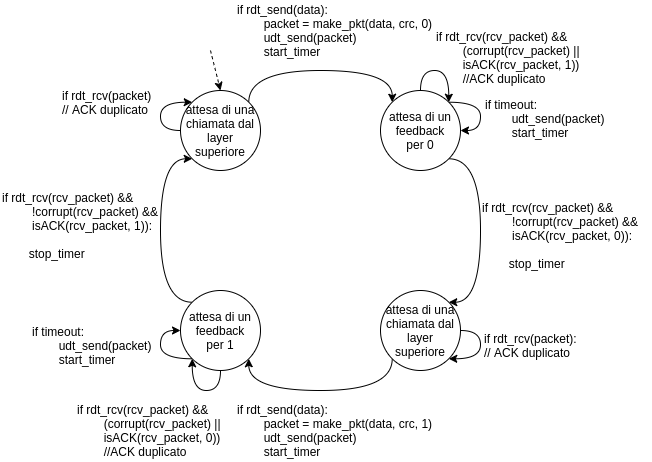
\includegraphics[width=340px]{images/3_Reti_connessione_diretta/rdt_3.0_sender.png}
    \caption{RDT 3.0 sender}
\end{figure}

\begin{figure}[H]
    \centering
    
\includegraphics[width=340px]{images/3_Reti_connessione_diretta/rdt_2.2_receiver.png}
    \caption{RDT 3.0 receiver}
\end{figure}

\subsection{Alternative allo stop-and-wait}
L' algoritmo visto è funzionante, tuttavia le performance sono molto scarse.
L' utilizzo del mezzo di comunicazione è bassissimo in quanto per ogni pacchetto inviato attendiamo che arrivi e che ci torni una conferma:

Es: link da 1Gbps, 15ms di propagazione, pacchetti da 8000bit: il delay di trasmissione è:
$$ d_{trans} = \frac{L}{R} = \frac{8000 bits}{10^9 bps} = 8 ms $$
l' utilizzo del mezzo è invece:
$$ U_{sender} = \frac{\frac{L}{R}}{RTT + \frac{L}{R}} = 0.00027 $$
Ci metto 30ms per inviare 1KB di dati, per un throughput di 267Kbps su un link che ne ammette 1Gbps.

Il problema risiede nell' utilizzo dell' approcio stop-and-wait, il tempo in attesa è tempo morto!

\subsubsection{Pipelining}
Un approccio migliore sarebbe quello di inviare più pacchetti in sequenza ed aspettare diversi ACK in risposta:
\begin{figure}[H]
    \centering
    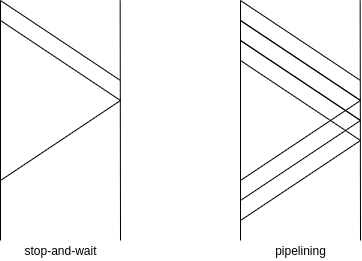
\includegraphics[width=200px]{images/3_Reti_connessione_diretta/stop-and-wait_pipelining.png}
\end{figure}

Per ottenere la pipeline bisogna apportare alcune modifiche al protocollo che abbiamo scritto:
\begin{itemize}
    \item bisogna avere delle sequenze più lunghe in quanto ci servono necessariamente più di 2 sequenze valide
    \item il trasmettitore e/o il ricevitore devono implementare meccanismi di buffering:
    \begin{itemize}
        \item il trasmettitore deve mantenere in memoria tutti i pacchetti che non hanno ancora ricevuto una conferma
        \item il ricevitore potrebbe implementare algoritmi di ri-ordinamento dei pacchetti out-of-order
    \end{itemize}
\end{itemize}
Possiamo avere due strategie di trasmissione:
\begin{itemize}
    \item Go-back-N
    \item Selective Repeat
\end{itemize}

\subsubsection{Go-back-N}
Il trasmettitore tiene in memoria una coda di pacchetti che non sono ancora stati confermati, i primi $N$ di questa lista formano la \emph{finestra}: quando invia pacchetti invia i pacchetti della finestra uno dopo l' altro in successione (in burst).

Quando il ricevitore li riceve invia un \emph{ACK cumulativo} cioè invia un ACK per l' ultimo pacchetto ricevuto correttamente in sequenza, non può inviare l' ACK per un pacchetto se non ha ricevuto correttamente anche tutti i precedenti, non possono esserci buchi.

Il trasmettitore mantiene un singolo timer per il pacchetto non confermato più vecchio, allo scadere di questo timer procede a reinviare la finestra a partire dal primo non confermato.
La finestra si sposta in avanti ogni volta che riceve un ACK per un pacchetto non ancora confermato.
Possono esserci ACK duplicati in quanto, appunto, se un pacchetto viene ricevuto corrotto il ricevitore provvederà ad inviare l' ACK dell'ultimo ricevuto correttamente.
\begin{figure}[H]
    \centering
    
\includegraphics[width=340px]{images/3_Reti_connessione_diretta/go-back-n_sender.png}
    \caption{Go-back-N sender}
\end{figure}
\begin{itemize}
    \item All' avvio la finestra parte dall' indice 1 ed il prossimo sequence\_number è uguale alla base in quanto non abbiamo pacchetti.
    Si noti che lasciamo lo 0 libero in modo che il ricevitore possa fare acknowledge su 0 per segnalare di non aver ricevuto il primissimo pacchetto.
    
    \item Alla chiamata dal layer superiore se la finestra non è piena provvediamo a creare un nuovo pacchetto con i dati da inviare e lo inviamo.
    Se la finestra era vuota, e quindi siamo al primo pacchetto della finestra, facciamo anche partire il timer.
    Se non c'è spazio nella finestra neghiamo la richiesta
    
    \item Se scatta il timer provvediamo a reinviare tutti i pacchetti nella finestra corrente
    
    \item Se riceviamo un pacchetto corrotto semplicemente non facciamo nulla
    
    \item Se riceviamo un pacchetto e non è corrotto usiamo il suo sequence\_number come nuova base della finestra, se coincide con la fine allora stoppiamo il timer, altrimenti lo facciamo ripartire in modo che adesso conti rispetto al pacchetto che ora è diventato il primo della finestra
\end{itemize}

\begin{figure}[H]
    \centering
    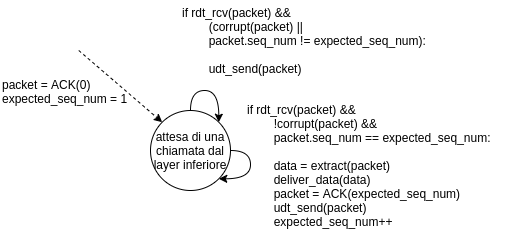
\includegraphics[width=340px]{images/3_Reti_connessione_diretta/go-back-n_receiver.png}
    \caption{Go-back-N receiver}
\end{figure}
\begin{itemize}
    \item All' avvio facciamo finta che l' ultimo pacchetto ricevuto avesse sequence\_number 0, quindi prepariamo il pacchetto di ACK su 0 mentre ci aspettiamo di ricevere il pacchetto con sequence\_number 1

    \item Se ricevo un pacchetto ed è corrotto o ha sequence\_number diverso da quello che mi aspetto provvedo a reinviare l' ultimo ACK prodotto
    
    \item Se ricevo un pacchetto non corrotto e con lo stesso sequence\_number che mi aspetto estraggo e consegno i dati che trasportava, creo l' ACK per quel sequence\_number e lo invio
\end{itemize}

Questo approccio ci permette di spostare la gran parte della complessità della trasmissione al trasmettitore, che infatti è più complesso, mentre lasciamo il minimo indispensabile al ricevitore.
In particolare questa implementazione non necessita nemmeno che il ricevitore abbia un buffer in quanto riceverà i pacchetti sempre nell' ordine corretto, se così non dovesse essere semplicemente verranno ignorati.

Questo approccio porta ad una grande ritrasmissione di pacchetti che magari sono arrivati correttamente ma ignorati in quanto out-of-order.


\subsubsection{Selective Repeat}
Il trasmettitore ha una coda di pacchetti che invia in sequenza (burst), riceve degli ACK per i singoli pacchetti e provvede a cancellare i pacchetti confermati da questa coda per far spazio ad altri.
Quando il timeout scade re-invia solo i pacchetti non confermati.

Il ricevitore quindi deve rispondere con i singoli ACK per i singoli pacchetti, deve anche avere un buffer interno in modo da mantere in memoria i pacchetti out-of-order per consegnarli al layer superiore nell' ordine corretto.

Anche in questo algoritmo possiamo pensare ad un concetto di finestra, per il trasmettitore la finestra parte dal primo pacchetto non confermato e va avanti per $N$ pacchetti.
In questo caso la finestra può avere dei buchi in quanto potrebbero esserci dei pacchetti di mezzo confermati ed altri no.

Anche il ricevitore ha un concetto di finestra che parte dal primo pacchetto che si aspetta di ricevere e va avanti per una dimensione $N$.
Se riceve un pacchetto che ha sequence\_number uguale a quello della base della finestra il contenuto viene subito spedito al layer superiore, altrimenti viene immagazzinato fino a che tutti i pacchetti prima di lui saranno ricevuti correttamente e spediti al layer superiore.


Queste due finestre saranno certamente \emph{out-of-sync} in quanto non sono concordate, questo potrebbe creare dei problemi se non tariamo bene le dimensioni del buffer e della finestra stessa:
\begin{figure}[H]
    \centering
    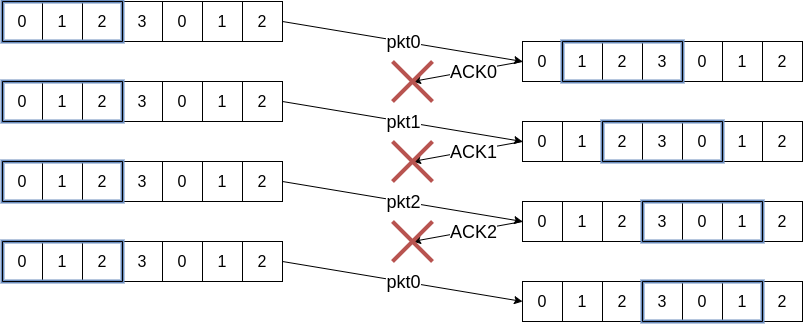
\includegraphics[width=300px]{images/3_Reti_connessione_diretta/window-desync.png}
\end{figure}
Supponiamo di avere la finestra di 3 elementi e di avere 4 sequence\_number:
\begin{itemize}
    \item TX invia il pacchetto 0, 1, 2
    \item RX riceve i pacchetti 0, 1, 2, risponde con gli ACK relativi e sposta la finestra
    \item Tutti gli ACK si perdono quindi TX non muove la sua finestra
    \item TX re-invia il pacchetto 0
    \item RX avendo la finestra spostata pensa che i pacchetti siano consecutivi e spedisce al layer superiore dei dati duplicati 
\end{itemize}

La dimensione della finestra deve quindi essere minore o uguale alla metà del numero dei sequence\_number che prevede la comunicazione.
Inoltre la larghezza della finestra dovrebbe evitare che il ricevitore debba memorizzare più pacchetti di quelli che effettivamente può memorizzare.
Possiamo scegliere un numero in base al RTT ed alla dimensione del buffer del ricevitore.

\subsection{Point to Point Protocol - PPP}
I Point to Point Data-Link protocols sono protocolli che permettono la comunicazione tra due elementi, un mittente ed un destinatario, connessi direttamente.
Alcuni esempi sono le linee ADSL e le connessioni dialup.
Tra questi il più utilizzato è stato il PPP, esso prevede:
\begin{itemize}
    \item \emph{Packet framing}: incapsula i datagrammi del livello rete in frame del livello data-link.
    Permette di trasportare tutti i protocolli di tipo rete, non solo IP, allo stesso tempo e di eseguire il demultiplexing verso il layer più alto.
    
    \item \emph{Bit transparency}: permette di trasportare nel frame qualsiasi pattern di bit
    
    \item Implementa la error detection ma non la correction
    
    \item \emph{Connection liveness}: si accorge e segnala al layer di rete se ci sono problemi sul collegamento
    
    \item \emph{network layer address negotiation}: gli endpoint possono mettersi d' accordo l' un l' altro per configurare i propri indirizzi di rete
\end{itemize}

Si noti che la mancanza di error recovery, flow control e data re-ordering può essere risolta implementandoli nei layer più in alto. 

\subsubsection{PPP Data frame}
Il frame del protocollo PPP è così composto:
\begin{figure}[H]
    \centering
    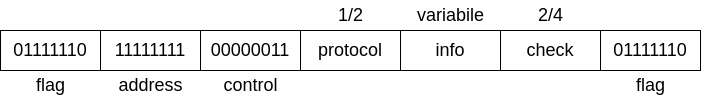
\includegraphics[width=300px]{images/3_Reti_connessione_diretta/ppp_data_frame.png}
\end{figure}
\begin{itemize}
    \item \emph{flag}: è il delimitatore del frame, si pone sia all' inizio che alla fine
    \item \emph{address}: è un campo inutilizzato che ha solo una possibile opzione
    \item \emph{control}: è un campo inutilizzato lasciato per futuri utilizzi
    \item \emph{protocol}: usato per specificare a quale protocollo di rete appartiene il frame
    \item \emph{info}: sono i dati da trasportare
    \item \emph{check}: CRC per la error detection
\end{itemize}

\subsubsection{Byte stuffing}
Dal momento che vogliamo poter trasmettere tutte le combinazioni di bit, per la data transparency, c'è bisogno di aggiustare la comunicazione affinché non ci siano problemi se nel campo info (ma non solo) dovesse comparire la sequenza del flag.
\begin{itemize}
    \item mittente: aggiunge la sequenza 01111101 prima di ogni byte flag
    
    \item destinatario: quando riceve la sequenza 01111101-flag rimuove il byte di escape e restituisce il byte successivo
\end{itemize}
NB: se si dovesse trasmettere lo stesso byte di escape lo si inserisce due volte affinché la prima volta venga scartato mentre la seconda venga trasmesso.

\subsubsection{PPP Link Control}
Prima di partire con la trasmissione dei dati i due endpoint possono negoziare alcune configurazioni:
\begin{itemize}
    \item configurazione del link PPP come la massima dimensione del frame ed un metodo di autenticazione, omissione dei campi address e control, ed altri.
    Questo viene fatto tramite il Link Control Protocol - LCP
    
    \item configurazione di rete come scambio e configurazione degli indirizzi IP
\end{itemize}


\subsection{Protocolli ad accesso multiplo}
Se volessimo interconnettere $N$ host differenti usando connessioni PPP avremmo necessità di $\frac{N(N-1)}{2}$ connessioni differenti.
Inoltre ogni host dovrebbe avere $N-1$ ingressi per il media, non è una soluzione che scala.
Per risolvere questo problema sono stati inventati i link ad accesso multiplo cioè dei media che sono condivisi tra più di 2 host.
Alcuni esempi sono il vecchio protocollo Ethernet ed il WiFi 802.11.

Per trasmettere bisogna darsi delle regole perché se due o più trasmissioni avvengono simultaneamente si ha una \emph{collisione} e quindi non si riceveranno dati corretti.
Il protocollo di accesso multiplo ideale dovrebbe prevedere:
\begin{itemize}
    \item pieno utilizzo: se solo un nodo vuole trasmettere esso deve poter trasmette alla massima capacità del canale
    \item fairness: se $M$ nodi vogliono trasmettere devono poterlo fare ad un rateo $\frac{R}{M}$
    \item completa decentralizzazione: non ci dovrebbero essere nodi speciali a coordinare la trasmissione
    \item semplicità
\end{itemize}

Abbiamo 3 classi di protocolli di accesso al mezzo:
\begin{itemize}
    \item a partizionamento del canale: si divide il canale in "pezzi" più piccoli, ad esempio in slot temporali, in canali di frequenza o su codice

    \item ad accesso casuale: il canale non è suddiviso, le collisioni sono ammesse ma si implementano dei meccanismi di recovery dalle collisioni.
    Quando un canale deve trasmettere trasmette a piena velocità.
    
    \item a turni: i nodi seguono un ordine ed attendono il loro turno per trasmettere, i nodi che hanno più da inviare prendono turni più lunghi
\end{itemize}

\subsubsection{TDMA - Time Division Multiple Access}
Si accede al media a turno, ogni stazione ha uno slot temporale di durata ben definita, di solito uguale al tempo di invio di un pacchetto.
Se una stazione non ha da trasmettere passa il suo slot in idle, quindi non si ha la fully utilization però si ha la fairness.
Non abbiamo una completa decentralizzazione in quanto serve qualcuno che dia l' ordine alle stazioni e dia la sincronizzazione.

\subsubsection{FDMA - Frequency Division Multiple Access}
Lo spettro del canale si suddivide in varie bande di frequenza, ad ogni stazione viene assegnato un singolo canale, se una stazione non ha da trasmettere rimane in idle sul suo canale.
Anche qui non abbiamo la fully utilization né la completa decentralizzazione, però è fair.

\subsubsection{CDMA - Code Division Multiple Access}
Ad ogni coppia di nodi viene assegnato un codice univoco per la trasmissione.
Tutte le comunicazioni avvengono simultaneamente ed ogni ricevitore può decodificare solo quella a lui destinata.
Permette la fully utilization e la fairness ma non è semplice.

\subsubsection{Slotted ALOHA}
Assumiamo che tutti i frame siano della stessa dimensione, dividiamo quindi il tempo in slot di dimensioni identiche a quelle necessarie per trasmettere un frame.
Quando un nodo ha dati da trasmettere lo fa all' inizio del primo slot temporale possibile, se 2 o più nodi trasmettono nello stesso slot tutti i nodi rilevano la collisione.
Quando ciò succede i nodi scelgono se provare a reinviare i frame nello slot successivo, scelgono casualmente di ritrasmettere con probabilità $p$, questa estrazione viene eseguita finché non riescono ad inviare i dati senza collisioni.
\begin{figure}[H]
    \centering
    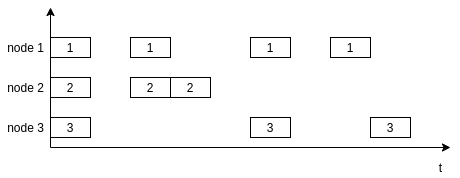
\includegraphics[width=250px]{images/3_Reti_connessione_diretta/slotted_aloha.png}
\end{figure}
In questa simulazione abbiamo 3 nodi che vogliono trasmettere e provano nel primo slot, essendoci una collisione devono tutti e 3 ritrasmettere.
Nello slot successivo nessuno dei 3 estrae la ritrasmissione, nel terzo slot ci riprovano 1 e 2 ma ancora una volta c'è una collisione.
Nel quarto slot finalmente il nodo 2 riesce a trasmettere da solo quindi il pacchetto viene consegnato intero, nessuna collisione.
Si continua così finché tutti e 3 non riescono a trasmettere da soli.

Tra i pro di questo algoritmo abbiamo:
\begin{itemize}
    \item se il nodo attivo è uno solo può trasmettere in ogni slot temporale, quindi utilizzo totale del mezzo
    \item alta decentralizzazione, l' unica cosa da negoziare è la durata di uno slot e l' inizio di ogni slot
    \item è semplice
\end{itemize}
tra i contro invece abbiamo:
\begin{itemize}
    \item ci sono tante collisioni quindi c'è tanto spreco di tempo
    \item in alcuni slot i nodi che vorrebbero trasmettere non lo fanno
    \item i nodi potrebbero detectare la collisione ben prima di finire di trasmettere i dati ma non lo fanno
    \item c'è da sincronizzarsi per avere tutti gli stessi slot
\end{itemize}

Calcoliamo l'efficienza: supponiamo che ci siano $N$ nodi con un po' di frame da inviare, ogni nodo trasmette in uno slot con probabilità $p$ uguale per tutti.
La probabilità che un nodo riesca a trasmettere correttamente in un frame è la probabilità che lui trasmetta $p$ e che tutti gli altri nodi non trasmettano $(1-p)^{N-1}$ quindi: $p(1-p)^{N-1}$.
La probabilità che qualsiasi nodo abbia successo è pertanto $Np(1-p)^{N-1}$.
La massima efficienza si ha con il $p*$ che massimizza $Np*(1-p*)^{N-1}$.
Per un numero alto di nodi eseguiamo il limite per $N \xrightarrow{} \infty$ ed otteniamo che l'efficienza massima è $\frac{1}{e} = 0.37$.
Si ha quindi una efficienza del canale del 37\%.

\subsubsection{Pure (unslotted) ALOHA}
La versione unslotted è più semplice, prevede l' eliminazione della sincronizzazione quindi si trasmette appena si hanno dei dati da trasmettere.
La probabilità di avere delle collisioni è quindi maggiore in quanto un frame inviato al tempo $t_0$ può collidere con i frame inviati nella finestra [$t_0-1$, $t_0+1$].

La probabilità di avere una comunicazione corretta è quindi la probabilità di essere gli unici che trasmettono nelle finestre [$t_0-1$, $t_0$], [$t_0$, $t_0+1$] cioè: $p(1-p)^{N-1}(1-p)^{N-1} = p(1-p)^{2(N-1)}$ per una efficienza massima di $\frac{1}{2e} = 0.18$

\subsubsection{CSMA - Carrier Sense Multiple Access}
Prima di trasmettere si ascolta il media, se c'è qualcuno che sta trasmettendo aspetto, altrimenti trasmetto tutto il frame.
Le collisioni continuano a verificarsi in quanto il tempo di propagazione ci offre una finestra di tempo nella quale possiamo ascoltare il mezzo, non sentire nulla e quindi iniziare la trasmissione, salvo poi accorgersi di avere una collisione.
In questo caso l' intero tempo della trasmissione del pacchetto è sprecato.

\subsubsection{CSMA/CD - Carrier Sense Multiple Access with Collision Detection}
Si usa la stessa tattica del CSMA ma quando si rileva una collisione si smette di trasmettere in modo da liberare il canale subito e non sprecare tempo.
La detection delle collisioni può essere eseguita in vari modi:
\begin{itemize}
    \item nelle reti su cavo si può misurare la potenza del segnale sul canale, se è maggiore della potenza che noi stiamo trasmettendo allora si ha una collisione
    
    \item anche nelle reti wireless si può usare la potenza del segnale tuttavia è più complesso in quanto entrano in mezzo anche le interferenze elettromagnetiche
\end{itemize}

Quando ci si accorge di una collisione si aumenta la potenza della trasmissione in modo da far accorgere prima anche gli altri nodi che stanno trasmettendo, questo si chiama \emph{jam signal}.

CSMA e la sua versione con CD garantisce la fullfilness in quanto possiamo trasmettere a pieno se siamo gli unici a dover trasmettere, è fair in quanto quando si incappa in una collisione ogni endpoint estrae un tempo casuale da attendere e quindi ci si da una specie di ordinamento permettendo comunque a tutti di trasmettere.
E' completamente decentralizzato in quanto nessun nodo ha più potere degli altri e non c'è una sincronizzazione.

Per bassi carichi è estremamente efficiente, tuttavia se il numero di host aumenta la sua efficienza cala drasticamente in quanto le collisioni aumentano.

\subsubsection{Polling}
E' un protocollo a turni in cui un nodo fa da \emph{master} e si occupa di interrogare i singoli nodi in sequenza chiedendo chi ha da trasmettere e dando singolarmente il permesso ad usare il media.

Essendo centralizzato abbiamo un single point of failure nel master, inoltre abbiamo un overhead perché il master deve interrogare singolarmente i nodi e dare loro il permesso.
Ogni nodo rileva una certa latenza perché deve aspettare di essere interrogato dal master prima di poter inviare.

\subsubsection{Token passing}
In una rete ad anello possiamo immaginare di avere un pacchetto che ci si passa tra gli host, chi ce lo ha in quel momento può trasmettere se ha pacchetti altrimenti provvede a passare in avanti il token.
E' come moderare un dibattito permettendo solo a chi ha il microfono in quel momento di parlare.

Non abbiamo single point of failure in quanto il token viene passato nella rete da un nodo all' altro e non ci sono nodi più importanti degli altri.

Abbiamo un overhead dettato dal passaggio del token ed anche una latenza in quanto devo aspettare di avere il token prima di poter trasmettere.

\subsection{Indirizzamento}
Per permettere ai protocolli ad accesso multiplo di funzionare e creare l' astrazione di connessioni punto-punto abbiamo la necessità di aggiungere un indirizzamento.
Ogni host ha un proprio indirizzo ed i frame che transitano nella rete riportano gli indirizzi del mittente e del destinatario.

Quando un host trasmette tutti gli altri ascoltano ma se non sono i diretti interessati droppano il pacchetto.

L' indirizzo è associato univocamente alla Network Interface Card dalla casa produttrice ed è un indirizzo su 48 bit (MAC address).
E' anche detto \emph{physical address}, \emph{link-layer address}.

Oltre ad un indirizzo univoco per ogni host prevediamo anche un indirizzo di \emph{broadcast} cioè un indirizzo che indica che tutti sono interessati a ricevere il messaggio.

\subsection{Local Area Network - LAN}
Sono reti che hanno la copertura di un edificio, una sua parte o alcuni edifici vicini geograficamente.
L' accesso è eseguito tramite Medium Access Control Protocol quindi media condivisi e si usa un indirizzamento basato su indirizzi fisici (MAC).
In generale le velocità vanno dai 10Mbps ai 10Gbps.

\subsubsection{Topologia delle LAN}
Possiamo avere diverse tipologie, le più comuni sono state:
\begin{figure}[H]
    \centering
    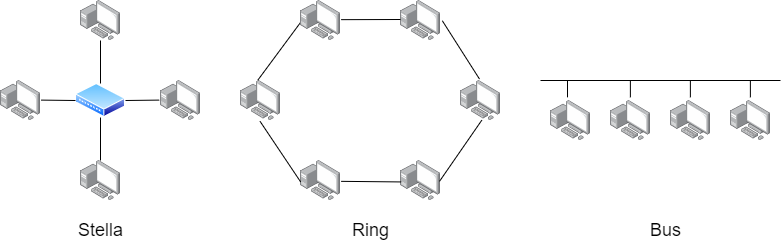
\includegraphics[width=330px]{images/3_Reti_connessione_diretta/network_topologies.png}
\end{figure}
NB: nella topologia a bus per evitare la riflessione del segnale si inserisce un resistore da $50 \Omega$ alla fine del cavo.

NB: la topologia a stella con un hub al centro non è altro che una topologia a bus in quanto l' hub si occupa di ripetere sugli altri canali ciò che riceve da uno singolo, per questo la stella è anche detta \emph{folded hub}.

\subsubsection{Indirizzi MAC}
Un indirizzo MAC è un indirizzo composto da 48 bit associato ad un adattatore di rete.
I primi 24 bit indicano il produttore dell' interfaccia di rete ed è assegnato dalla IEEE, gli ultimi 24 bit invece sono assegnati dal produttore alla singola interfaccia.

Per rappresentarli semplicemente si usa una notazione esadecimale.
Il MAC di broadcast è per convenzione FF:FF:FF:FF:FF:FF.

Questi indirizzi sono pertanto univocamente associati e sono portabili attraverso le diverse reti a differenza degli indirizzi IP che hanno senso solo in una rete.

\subsection{Ethernet}
E' la tecnologia di accesso tramite cavo più utilizzata oggigiorno, è economica, semplice da utilizzare e permette di avere velocità tra i 10Mbps ed i 10 Gbps.

\begin{figure}[H]
    \centering
    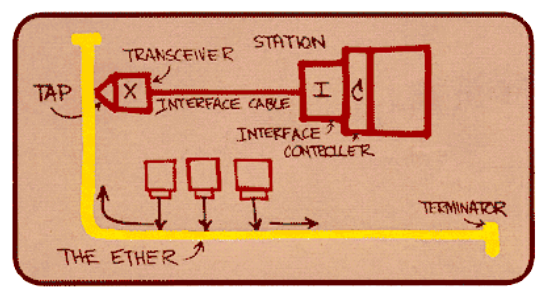
\includegraphics[width=200px]{images/3_Reti_connessione_diretta/Metcalfe_ethernet.png}
\end{figure}
In foto lo sketch dell'interfaccia di rete Ethernet pensata da Bob Metcalfe.

Nella topologia a bus abbiamo tutti gli host connessi ad un singolo bus e tutti gli host sono nello stesso dominio di collisione.

Nella topologia a stella invece ogni host ha un collegamento dedicato verso l' hub centrale ma essendo l' hub un ripetitore di segnale si continua ad avere un singolo dominio di collisione.

\subsubsection{Hub}
L' hub è un dispositivo di rete che lavora sul layer fisico, è banalmente un ripetitore di segnale: tutti i bit che arrivano in una interfaccia vengono ripetuti su tutte le altre interfacce alla stessa velocità di ingresso.
Questo significa che qualsiasi nodo connesso all' hub può collidere con tutti gli altri.
Non c'è un concetto di buffering, tantomeno un metodo di accesso CSMA/CD.

\subsubsection{Switched Star topology}
Oggigiorno si usano delle topologie a stella con al centro un apparato di rete chiamato \emph{switch}.
Questo dispositivo lavora al livello data-link quindi riesce a comprendere i protocolli di accesso ed i frame.
Permette anche di bufferizzare i frame in ingresso e di spedirli in uscita ai diretti interessati dopo aver controllato che il media sia libero e che quindi non ci sia il rischio di collisioni.
Permette inoltre di inviare il traffico direttamente al destinatario senza dover passare per una ripetizione in broadcast.

\subsubsection{Struttura di un frame ethernet}
\begin{figure}[H]
    \centering
    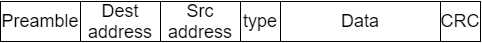
\includegraphics[width=250px]{images/3_Reti_connessione_diretta/ethernet_frame.png}
\end{figure}
\begin{itemize}
    \item preambolo: 7 byte con valore 10101010 ed 1 byte con valore 10101011, sono usati per sincronizzare la velocità del ricevitore con quella del trasmettitore
    
    \item indirizzo di destinazione: è il MAC address di chi deve ricevere il frame.
    E' inviato per primo in modo che chiunque stia ascoltando e non è il destinatario possa smettere di immagazinare i dati trasmessi
    
    \item indirizzo sorgente: è il MAC address di chi sta inviando il frame
    
    \item tipo: indica il protocollo di livello superiore al quale recapitare i dati incapsulati nel frame.
    Ora principalmente IP ma non è detto
    
    \item CRC: usati per l' error detecion del frame.
    Non fa error correction
\end{itemize}
Un frame ethernet è grande almeno 64byte, cioè 512 bit.

\subsubsection{Codifica Manchester}
Per trasmettere i dati sulla linea si utilizza la codifica manchester:
\begin{figure}[H]
    \centering
    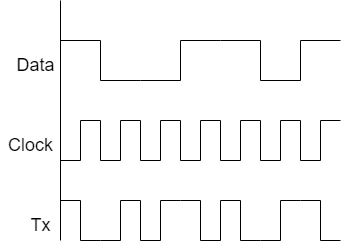
\includegraphics[width=220px]{images/3_Reti_connessione_diretta/manchester_encoding.png}
\end{figure}
il flusso dei dati viene xorato con il clock e si trasmette il risultato.
Questa codifica è utile in quanto permette ai clock del ricevitore e del trasmettitore di rimanere sincronizzati per tutta la durata della trasmissione, inoltre in ogni bit c'è una transizione dall' alto al basso o dal basso all' alto, quindi senza conoscere il centro dell' impulso per campionare possiamo rilevare questa transizione.

Per estrarre il clock dai dati il ricevitore utilizza un anello ad aggancio di fase.
Di fatto il preambolo è una porzione del frame di pertinenza del layer fisico.

\subsubsection{Proprietà del protocollo Ethernet}
Ethernet è un protocollo connectionless quindi non prevede un handshake iniziale, tantomeno una chiusura della connessione alla fine della trasmissione.

E' un protocollo non affidabile, non ci sono ACK né NAK, è un flusso continuo di datagrammi che possono anche avere dei gap.
Questa non affidabilità può essere poi aggiustata dai protocolli dei layer superiori.

Usa una politica CSMA/CD per l' accesso al mezzo.

\subsubsection{CSMA/CD di Ethernet}
\begin{itemize}
    \item La scheda di rete riceve dei dati dal layer di rete, crea un frame

    \item se la NIC rileva il canale libero per il tempo di 96 bit allora inizia la trasmissione del frame.
    Se il canale è occupato aspetta finché non riesce a vederlo libero per 96 bit time
    
    NB: quanto vale un bit time? Supponiamo di trasmettere ad 10Mbps allora $\frac{1}{10^{7}} = 0.1\mu s$
    
    \item se la NIC riesce ad inviare il frame completamente ha finito con quel frame
    
    \item se invece rileva una collisione durante la trasmissione abortisce ed invia 48 bit di segnale di disturbo in modo da far accorgere anche gli altri host che stanno trasmettendo
    
    \item dopo aver interrotto la trasmissione aspetta un \emph{exponential backoff} cioè all' n-esima collisione sceglie $K$ casualmente nell' insieme $\{0, 1, 2, \_, 2^{m}-1\}$ con $m=min(n, 10)$ ed aspetta per $K \cdot 512$ bit time per poi tornare ad ascoltare il mezzo per la trasmissione
\end{itemize}
L' exponential backoff è un metodo per adattarsi al carico di trasmissione del mezzo, se dopo un paio di tentativi continuo ad avere collisioni vuol dire che devo provare ad aspettare molto di più.

Dopo 17 collisioni successive il frame viene droppato direttamente.

\subsubsection{Standard Ethernet}
Ci sono diversi standard ethernet a diverse velocità e per diversi media fisici:
\begin{figure}[H]
    \centering
    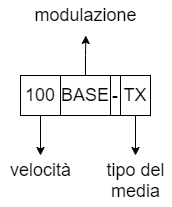
\includegraphics[width=100px]{images/3_Reti_connessione_diretta/standard_ethernet.png}
\end{figure}

\section{Packet Switched Networks}
Sono reti locali basate sull' utilizzo degli switch.
\subsection{Switch}
Sono device di rete che lavorano sul layer data-link, sono più intelligenti degli hub ed hanno un ruolo attivo nello smistamento del traffico.

Permettono infatti di leggere i frame ethernet, tenerli in memoria e instradarli \emph{selettivamente} verso una o più interfacce di uscita attravero il MAC address di destinazione.

Sono dispositivi trasparenti cioè gli host non sanno che sono presenti nella rete e non devono avere comportamenti particolari quando sono presenti; sono elementi plug \& play cioè se inseriti in una rete funzionano di default senza alcune particolari configurazioni.

Sono self-learning cioè imparano da soli quali host sono connessi ad essi in modo da instradare il traffico.

Suddividere il dominio di collisione permette di avere trasmissioni \emph{simultanee} verso diversi host della rete in quanto ogni host ha una connessione diretta e dedicata verso uno switch.

\subsubsection{Switch table e self-learn}
Abbiamo detto che uno switch impara da solo quali host sono connessi a lui, questo processo funziona in diversi step:
\begin{itemize}
    \item lo switch riceve un frame su una interfaccia
    \item prende il MAC address di destinazione e cerca nella tabella di switching verso quale porta è connesso l' host destinatario
    \item instrada il frame verso quella interfaccia
    \item se non è presente una entry nella tabella il frame viene instradato su \emph{tutte} le interfacce dello switch
    \item aggiunge un record nella switch table in cui associa il MAC address sorgente alla interfaccia di arrivo
\end{itemize}

Supponiamo ora che uno degli host si disconnetta dal suo switch e si riconnetta ad un altro, se le tabelle di switching fossero statiche, una volta create, l' host rimarrebbe isolato.
Per evitare questo inconveniente le entry della tabella hanno una scadenza.


\subsection{Switched Ethernet}
Vari switch possono essere connessi tra di loro in livelli gerarchici:
\begin{figure}[H]
    \centering
    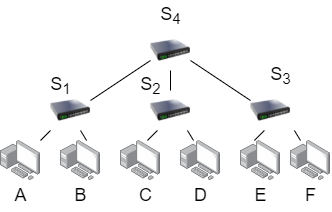
\includegraphics[width=200px]{images/4_Switched_Networks/layered_switch.png}
\end{figure}
Quest strutture sono utili per organizzare le reti in base alla posizione.
Se A vuole inviare un frame ad E invierà il frame inizialmente ad $S_1$, se questo ha la entry nella tabella lo invierà ad $S_4$ altrimenti lo invia su tutte le sue interfacce e così via per ogni switch.

Questo genere di rete permette l' eliminazione delle collisioni e quindi un aumento delle performance.
Inoltre permette di supportare diversi tipi di link in quanto gli switch possono avere diversi tipi di interfacce.
Sono semplici da gestire perché se c'è un link danneggiato si può disconnetterlo direttamente dallo switch e sostituirlo.
Aumenta anche la security perché grazie all' instradamento selettivo si limita di molto lo sniffing dei pacchetti (si può sempre eseguire un poisoning delle tabelle di switching).


\subsection{VLANs}
Riprendiamo la topologia gerarchica precedente, notiamone alcuni problemi:
\begin{itemize}
    \item il traffico di broadcast è globale per tutta la rete, nonostante logicamente siano 3 reti diverse
    \item abbiamo un utilizzo inefficiente degli switch, in genere hanno molte porte ma noi ne usiamo solo alcune perché vogliamo avere una divisione della rete
    \item se un utente di una rete si spostasse di reparto ma volesse continuare ad essere connesso alla stessa sottorete di prima non potrebbe farlo senza tirare nuovi cavi
\end{itemize}
Per risolvere questi ed altri problemi sono state inventate le VLAN - Virtual LAN.

\subsubsection{Port-based VLAN}
Si raggruppano le porte di uno switch (tramite opportune configurazioni) in modo che un singolo switch fisico operi come più switch virtuali.
Con questa implementazione otteniamo:
\begin{itemize}
    \item isolamento del traffico: i frame che arrivano da una VLAN non possono andare nell' altra senza passare per un router (quindi forwarding a livello rete)

    \item appartenenza dinamica: le singole porte dello switch possono cambiare VLAN alla quale sono assegnate tramite opportuna configurazione
\end{itemize}

NB: posso anche segnare l' appartenenza di un host ad una VLAN attraverso il suo indirizzo MAC.

\subsubsection{VLAN tra più switch}
Per permettere a diversi switch di instradare traffico sulle VLAN c'è bisogno di un nuovo protocollo che modifichi i frame aggiungendo le informazioni sulle VLAN.
Possiamo configurare le porte che connettono i due switch come \emph{porte trunk} cioè come porte che parlano il protocollo 802.1Q.

Mettiamo in comparazione il formato dei frame ethernet e 802.1Q:
\begin{figure}[H]
    \centering
    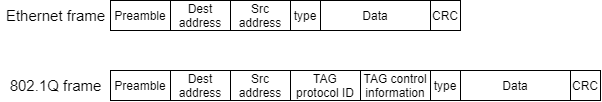
\includegraphics[width=330px]{images/4_Switched_Networks/802.1Q_frame.png}
\end{figure}
i campi in più sono:
\begin{itemize}
    \item Tag protocol identifier: indicano il protocollo usato per le VLAN
    \item Tag control information: contiene l' identificativo della VLAN (12 bit) ed altre informazioni
\end{itemize}
Ovviamente viene ricomputato il CRC su tutto il nuovo frame.

\subsection{Wide-Area Packet-Switched Networks}
Con solamente gli switch possiamo creare delle reti abbastanza grandi in cui l'indirizzamento è basato sull' indirizzo fisico (MAC address) e l' instradamento è effettuato dagli switch attraverso le loro tabelle.

Possiamo creare due tipi di servizi su queste reti:
\begin{itemize}
    \item connectionless: ogni pacchetto è gestito singlarmente, detto anche servizio a datagramma
    \item con connessione: si crea un circuito virtuale prima della trasmissione e tutti i pacchetti poi lo seguono per arrivare a destinazione
\end{itemize}

\subsubsection{ATM - Asynchronous Transfer Mode}
E' uno standard risalente agli anni 90 che aveva come scopo quello di permettere il trasporto di voce, video e dati in maniera efficiente per tutti questi tipi di servizi.

E' un sistema ad instradamento di pacchetti che usa canali virtuali, i pacchetti sono di dimensione fissa e sono chiamati \emph{cells}.

Offre 4 servizi in base al tipo di traffico da instradare:
\begin{itemize}
    \item CBR: constant bit rate
    \item VBR: variable bit rate
    \item ABR: available bit rate
    \item UBR: unspecified bit rate
\end{itemize}

Essendo basato su un circuito virtuale prima di trasmettere i dati si deve effettuare una chiamata in modo da costruire il canale, alla fine invece bisogna distruggerlo, ciò va fatto per ogni flusso di dati che si vuole inviare.

Ogni pacchetto trasporta l' identificativo del canale virtuale, non l' indirizzo del destinatario, ogni switch che incontra nel suo percorso legge questo identificativo e sa verso quale interfaccia instradarlo in quanto conosce il percorso che deve prendere.

Per rendere il servizio predicibile i dispositivi di rete intermedi possono allocare delle risorse al singolo canale virtuale.

Il pacchetto che viene instradato sul canale virtuale oltre a contenere l' identificativo del segnale mantiene anche il numero del link, ogni link nel canale ha un numero univoco che lo identifica e la sequenza di questi numeri è il percorso che costituisce il canale.
Quando uno switch si vede arrivare un pacchetto controlla il numero di link che contiene e l' interfaccia di ingresso, consulta la sua tabella di forwarding e legge l' interfaccia di uscita ed il numero di link di uscita, usa questo numero per sostituire il numero di link che contiene il pacchetto.

Per fare ciò ogni switch deve mantenere in memoria lo stato delle connessioni, quindi è un protocollo stateful.

\subsection{Datagram service}
Non ha bisogno di un setup iniziale, gli switch non devono mantenere informazioni circa lo stato delle connessioni, i singoli pacchetti possono seguire percorsi diversi dalla sorgente alla destinazione in base a metriche opportune per scegliere i link.
I pacchetti vengono indirizzati sulla base del solo indirizzo di destinazione.

\subsection{Virtualizzazione di una rete}
Tutto questo layer si può vedere come una astrazione di una connessione punto-punto.
Il livello superiore chiede di inviare pacchetti verso un certo host destinatario, non gli importa se i due siano connessi direttamente o ci siano altri dispositivi nel mezzo, ciò che vede il layer superiore è una connessione punto-punto.


\section{Internetworking}
Una inter-network è una rete che mette in collegamento altre reti: \emph{è una rete di reti}.
Ognuna delle reti che partecipa usa tecnologie diverse, diverse caratteristiche fisiche, diversi formati dei frame e diversi schemi di indirizzamento.

\begin{figure}[H]
    \centering
    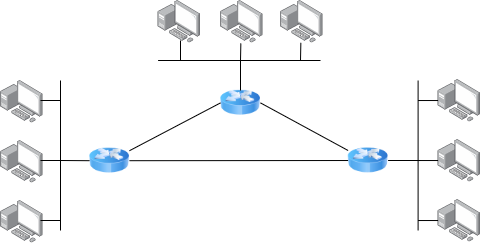
\includegraphics[width=200px]{images/5_Internetworking/inter-network.png}
\end{figure}

A fare la traduzione tra due o più reti c'è un interprete detto \emph{router} che si occupa di parlare queste "lingue diverse" e permettere il transito delle informazioni.

Per permettere questa interoperabilità creiamo un altro layer che ci permetta di creare l' astrazione che tutte queste reti diverse siano una singola rete unica ed omogenea.
Il protocollo principale di internetworking per Internet è IP.

\subsection{Introduzione}
Permette il trasferimento in maniera trasparente dei pacchetti, \emph{datagram}, dal nodo sorgente al nodo destinatario attraverso le varie reti intermedie.
Dal lato sorgente incapsula i dati ricevuti dal layer di trasporto, al lato destinatario invia i dati ricevuti al livello di trasporto.

Questo protocollo deve essere implementato in tutti gli host ed anche nei router in quanto, appunto, devono provvedere al forward, quindi dovranno poter interpretare le informazioni presenti nell' header del datagramma.


\subsubsection{Routing \& Forwarding}
\begin{itemize}
    \item forwarding: muove i pacchetti dall' interfaccia di ingresso del router all' interfaccia di uscita corretta
    \item routing: determina il percorso ottimale da far seguire al pacchetto per farlo arrivare a destinazione.
    Prevede l' utilizzo di algoritmi di routing cercando di ottimizzare una o più metriche.
\end{itemize}

Per fare una analogia: il routing è il processo di pianificare un viaggio partendo da una sorgente ed una destinazione, il forwarding è il processo di seguire il percorso step-by-step.

Gli algoritmi di routing permettono di generare la tabella di forwarding che ci dice in base all' indirizzo di destinazione quale uscita prendere.
Il forwarding poi usa questa tabella per indirizzare i pacchetti.

\subsubsection{Tipi di servizio}
Discerniamo i tipi di servizio in base al tipo di connessione:
\begin{itemize}
    \item connectionless: ogni pacchetto è gestito individualmente, si dice protocollo a datagramma
    \item connection: si sceglie un percorso predefinito all' inizio, creando di fatto un canale di comunicazione. Questo canale va poi anche deallocato alla fine del trasferimento 
\end{itemize}

I processi connectionless sono più veloci in quanto non c'è la costruzione della connessione, tantomeno il teardown.
Inoltre ogni router deve anche mantenere in memoria meno informazioni non dovendo sapere come si compone il circuito.
I pacchetti possono poi prendere strade diverse, il che è positivo se la struttura della rete cambia o se alcuni link diventano più occupati di altri.

Nel caso dei datagrammi la complessità è spostata agli estremi della rete, nei protocolli a connessione la complessità è nella rete stessa.
La rete a datagrammi può adattarsi, è più flessibile e permette link di diversi tipi e caratteristiche.

\subsubsection{Modelli di servizio}
Alcuni servizi che sarebbe comodo avere potrebbero essere:
\begin{itemize}
    \item affidabilità nella consegna
    \item consegna in ordine
    \item garanzia per una banda minima e di un delay massimo
    \item security nei fronti di confidenzialità, integrità ed autenticazione
\end{itemize}
Il modello di servizio di Internet è conosciuto come \emph{best-effort} cioè si fa il minimo indispensabile per recapitare i dati.
Non ci garantisce niente di ciò che richiediamo, tuttavia ci permette di costruire tutte queste caratteristiche nei layer superiori.

\subsection{Architettura di un router}
Il router svolge due principali funzioni:
\begin{itemize}
    \item forwarding dei datagrammi
    \item eseguire algoritmi/protocolli di routing interfacciandosi con gli altri router della rete
\end{itemize}

\begin{figure}[H]
    \centering
    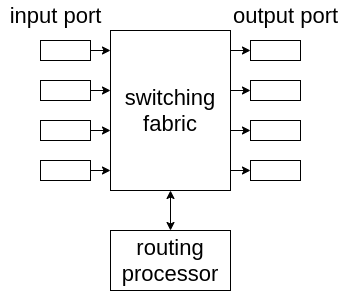
\includegraphics[width=200px]{images/5_Internetworking/router-architecture.png}
\end{figure}

\subsubsection{Porta di ingresso}
Deve "parlare" i primi 3 layer dello stack TCP/IP in quanto deve leggere i bit dal media, eseguire la error detection estrando il frame, successivamente estrarre il datagram IP.
Si guarda l' indirizzo di destinazione, si sceglie quale porta usare per rispedire il pacchetto e si inserisce il datagramma nel buffer interno della porta di uscita.
Se non è il primo datagram che arriva allora viene inserito nella coda della porta di ingresso finché non è il suo turno.

La commutazione tra ingresso e uscita può essere eseguita in modi diversi:

\begin{itemize}
    \item memoria condivisa:
    ogni interfaccia è costituita da un processore che ha accesso alla memoria come tutti gli altri
    \begin{figure}[H]
        \centering
        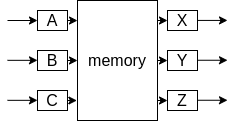
\includegraphics[width=150px]{images/5_Internetworking/memory.png}
    \end{figure}
    Non è molto performante a causa degli innumerevoli accessi alla memoria.

    \item via bus: i datagrammi vengono inviati su un bus condiviso tra tutte le interfacce.
    \begin{figure}[H]
        \centering
        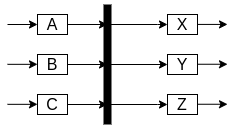
\includegraphics[width=150px]{images/5_Internetworking/bus.png}
    \end{figure}
    Anche questo approccio è lento perché bisogna gestire gli accessi al bus in mutua esclusione

    \item crossbar: un circuito più complesso che permette di collegare ogni interfaccia in ingresso con ogni interfaccia di uscita singolarmente
    \begin{figure}[H]
        \centering
        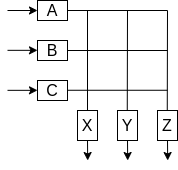
\includegraphics[width=150px]{images/5_Internetworking/crossbar.png}
    \end{figure}
    E' più complessa ma più efficiente
\end{itemize}

\subsubsection{Porta di uscita}
Questa interfaccia legge i dati dal suo buffer e provvede ad inviarli.
La coda può essere gestita in maniera arbitraria, non per forza First-Come-First-Served, si potrebbe ad esempio dare una priorità ad alcuni datagrammi che necessitano una qualità di servizio maggiore.

\subsection{Internet Protocol - IP}
E' di fatto il principale protocollo di livello Network, si serve tuttavia di informazioni generate da altri protocolli di livello rete.
Vediamo come si compone il datagramma IP (versione 4):
\begin{figure}[H]
    \centering
    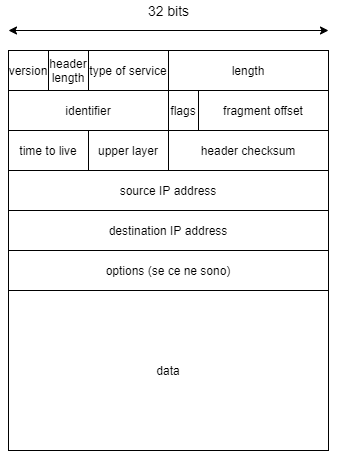
\includegraphics[width=200px]{images/5_Internetworking/ip_datagram_format.png}
\end{figure}

\begin{itemize}
    \item version: indica la versione del protocollo IP da usare (possiamo usare solo 4)
    \item header length: indica la dimensione dell' header in parole da 32 bit
    \item type of service: indica il quality of service dei dati che si stanno trasportando, usati per fare differenziazione del traffico e dare priorità
    \item length: lunghezza totale del datagramma
    \item identifier, flags, fragment offset: usati per la frammentazione
    \item time to live: indica il numero massimo di hop che il datagramma può ancora fare, ogni hop che riceve il pacchetto decrementa questo campo, una volta arrivato a 0 si droppa automaticamente e si notifica il nodo sorgente dell' accaduto 
    \item upper layer: indica il layer superiore al quale consegnare i dati di questo datagramma
    \item header checksum: checksum dell' header
    \item source IP address: indirizzo IP sorgente
    \item destination IP address: indirizzo IP destinatario
    \item options: informazioni aggiuntive sul pacchetto o sul forwarding come ad esempio (in genere non ci sono):
    \begin{itemize}
        \item source routing: si inseriscono gli hop sui quali instradare il pacchetto, indicando di fatto quale percorso deve seguire il pacchetto
        \item timestamp: si può aggiungere un timestamp nel pacchetto
    \end{itemize}
    \item data: dati da incapsulare provenienti dal layer superiore
\end{itemize}
E' necessario formulare un nuovo tipo di pacchetto per rendere interoperabili tutti i tipi di reti tra di loro, se usassimo il frame non ci sarebbe interoperabilità perché ogni rete definisce il suo modello di frame in base alla tecnologia ed il protocollo che usa, avendo questo formato invece possiamo rendere interoperabili tutte le reti in quanto per navigare all' interno della stessa rete usiamo frame, per navigare tra le diverse reti invece usiamo il formato IP.

\subsubsection{Frammentazione}
Un datagramma IP può essere grande al massimo 64Kbyte, la massima dimensione di un frame ethernet è di 1500 byte, non possiamo quindi inviare un datagramma IP usando un solo frame ethernet.
Si ricorre quindi alla frammentazione del datagramma cioè si divide il datagramma in porzioni più piccole inviate singolarmente e poi ricostituite alla ricezione.

Ogni frammento viene trattato come un datagramma quindi avrà lo stesso header di quello originale ma ora si popolano anche i campi per la frammentazione.
\begin{itemize}
    \item l' ID prende lo stesso ID del datagramma originale
    \item il fragment flag (more fragment bit) prende 1 se il datagramma non è l' ultimo, prende 0 se è l' ultimo da inviare
    \item L' offset prende il numero dei byte inviati fino ad ora e lo divide per 8. Questo perché non abbiamo 16 bit per questo campo ma solo 13, si indica quindi il punto nel datagramma originale nel quale inserire il frammento corrente piuttosto che il numero della posizione.
\end{itemize}

Supponiamo di voler inviare un datagramma da 5000 byte su un media che ha un MTU (max transmission unit) di 1500 byte, procediamo a frammentare:
\begin{figure}[H]
    \centering
    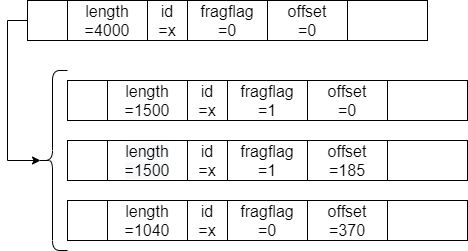
\includegraphics[width=300px]{images/5_Internetworking/fragmentation_example.png}
\end{figure}
\begin{itemize}
    \item tutti i frammenti prendono lo stesso id
    \item i primi due frammenti prendono il fragment flag ad 1, l' ultimo a 0
    \item il primo prende dimensione 1500byte (1480 di dati e 20 di header) ed offset 0
    \item il secondo prende dimensione 1500byte e come offset $\frac{byte\_inviati}{8} = \frac{1480}{8} = 185$
    \item il secondo prende dimensione 1040byte (i rimanenti) e come offset $\frac{2960}{8} = 370$
\end{itemize}
Se dopo aver frammentato un altro router trova un media con MTU ancora minore, può frammentare ancora di più.

Se ci accorgiamo che non abbiamo tutti i frammenti non possiamo fare altro che buttare tutto quanto e chiedere all' host sorgente di reinviare tutto quanto, questo perché non possiamo sapere chi ha eseguito la frammentazione quindi non sappiamo a chi chiedere.
Inoltre questo approccio è coerente con la filosofia best effort del protocollo.


\subsection{IP addressing}
Un  indirizzo IP è un valore composto da 32 bit ed identifica un host connesso nella rete, o meglio una interfaccia di un host connessa nella rete, solitamente si rappresenta e si legge in notazione decimale puntata.

Un indirizzo IP è detto strutturato in quanto si compone di due parti:
\begin{itemize}
    \item subnet part: i bit più alti
    \item host part: i bit più bassi
\end{itemize}
Una sottorete è l' insieme delle interfacce con la stessa porzione di sottorete nell' indirizzo IP che possono parlare tra di loro senza neanche l' utilizzo del router.
\begin{figure}[H]
    \centering
    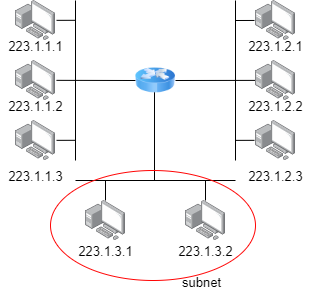
\includegraphics[width=200px]{images/5_Internetworking/subnet.png}
\end{figure}

Questa organizzazione è di tipo gerarchico, conoscendo la parte di rete di un indirizzo IP abbiamo informazioni che riguardano la posizione di un nodo in quanto tutti gli elementi di una stessa rete saranno connessi tra di loro.

\subsubsection{Classi degli indirizzi IP}
Suddividiamo gli indirizzi IP in alcune categorie:
\begin{figure}[H]
    \centering
    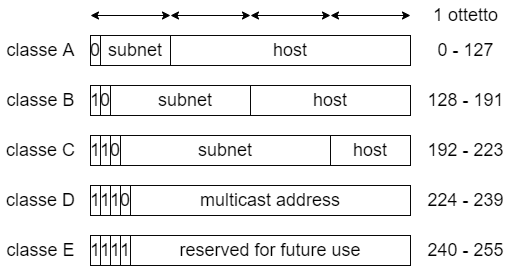
\includegraphics[width=300px]{images/5_Internetworking/ip_classes.png}
\end{figure}
Si noti che più bit di host ci sono e più host può accogliere una rete, ma meno reti ci possono essere di quel tipo, per esempio le reti di tipo B possono essere $2^{14}$ ed ogni rete può accogliere $2^{16} - 2$ host. (il perché del -2 lo vedremo più avanti).

Rimanere fissi con le classi tuttavia comporta un certo spreco di indirizzi: se una società chiede indirizzi per 1000 dispositivi siamo costretti ad utilizzare una rete di classe B che però potrebbe accogliere fino a 65534 host, abbiamo uno spreco immane.

\subsubsection{Indirizzamento classless}
Per ottimizzare l' utilizzo degli indirizzi IP smettiamo di considerare le classe e passiamo ad un indirizzamento con un numero di bit per la subnet variabile a piacere, ricorriamo quindi al CIDR - Classless InterDomain Routing.
Rappresentiamo gli indirizzi IP in questa forma: a.b.c.d/x dove x indica il numero di bit della porzione di rete.

Es: 200.23.16.0/23 con questo indirizzo possiamo accogliere fino a 510 dispositivi.


\subsubsection{Indirizzi riservati}
Ci sono degli indirizzi che non possono essere assegnati perché sono riservati per alcuni scopi:
\begin{table}[H]
    \centering
    \begin{tabular}{c|c|l}
        Subnet & Host & Descrizione \\
        \hline
        0 & 0 & Indica questo nodo \\
        $x$ & 0..0 & Indirizzo della rete $x$ \\
        $x$ & 1..1 & Indirizzo di broadcast \\
        1..1 & 1..1 & Indirizzo di broadcast ristretto \\
        127 & $x$ & Indirizzo di loopback \\
    \end{tabular}
\end{table}
L' indirizzo di broadcast è un indirizzo che indica che il pacchetto deve essere inviato a tutti gli host nella rete locale.
L' indirizzo di broadcast ristretto è l' indirizzo di broadcast che si usa quando non si sa l' IP della rete.
L' indirizzo di loopback è un indirizzo che punta alla macchina stessa, spesso usata dai programmatori per testare le proprie applicazioni di rete senza ricorrere ad una vera rete.


\subsubsection{Gerarchia degli indirizzi}
Sia usando l' indirizzamento classful che quello classless abbiamo la possibilità di ricorrere ad una gerarchia degli indirizzi: supponiamo di avere 8 reti con indirizzi: 200.23.16.0/23, 200.23.18.0/23, \_, 200.23.30.0/23 tutte gestite da un determinato ISP per conto delle singole 8 organizzazioni.
I router dell' ISP devono avere necessariamente una entrata nella tabella di routing per ogni rete singola, i router della rete Internet invece posso salire di gerarchia ed usare solamente un singolo record per la rete 200.23.26.0/20.
\begin{figure}[H]
    \centering
    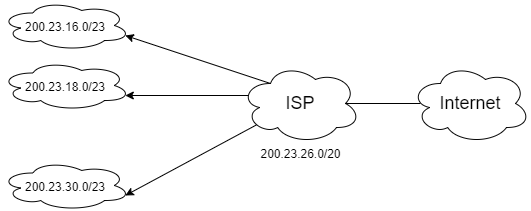
\includegraphics[width=300px]{images/5_Internetworking/hierarchical_addressing.png}
\end{figure}


\subsubsection{Ottenere un blocco di indirizzi}
Per ottenere un blocco di indirizzi ci si interfaccia con un Internet Service Provider, ogni ISP a sua volta chiede ad un ISP più grande e così via fino ad arrivare al provider di più alto livello che è ICANN - Internet Corporation for Assigned Names and Numbers.
Questa organizazione alloca gli indirizzi, gestisce i DNS ed assegna i nomi dei domini risolvendo eventuali dispute.

\subsubsection{Ottenere un indirizzo}
Un singolo host per avere un indirizzo può:
\begin{itemize}
    \item utilizzare un indirizzamento statico: si chiede al responsabile della rete la configurazione del singolo dispositivo
    \item utilizzare un indirizzamento dinamico: si utilizza un servizio della rete locale noto come DHCP - Dynamic Host Configuration Protocol che si occupa di assegnare gli IP agli host che lo richiedono utilizzando il protocollo stesso.
    Questa seconda via è plug-and-play in quanto basta che l' host si connetta alla rete e richieda in broadcast un indirizzo libero.
\end{itemize}

\subsection{DHCP}
E' il protocollo che permette di configurare i nuovi host che entrano nella rete.
La configurazione avviene tramite il così detto: \emph{four-way handshake} cioè uno scambio di 4 messaggi tra l' host che vuole configurarsi ed il server DHCP.
Questo scambio di messaggi è così operato:
\begin{itemize}
    \item il client invia in broadcast una richiesta "DHCP discover" nella quale richiede i servigi del server DHCP.
    In questa richiesta il client inserisce:
    \begin{itemize}
        \item come IP sorgente 0.0.0.0 porta 68
        \item come IP destinatario 255.255.255.255 porta 67
        \item come yiaddr (Your IP Address) 0.0.0.0
        \item inserisce un transaction ID generato casualmente
    \end{itemize}
    Essendo questo messaggio in broadcast tutti gli host nella sottorete lo ricevono, quindi anche un eventuale server DHCP

    \item il server risponde con un messaggio "DHCP offer" nel quale inserisce:
    \begin{itemize}
        \item come IP sorgente l'effettivo IP del server e porta 67
        \item come IP destinatario 255.255.255.255 porta 68
        \item come yiaddr l' indirizzo che si sta offrendo al client
        \item inserisce anche un lifetime cioè la durata temporale dell' associazione host-IP
        \item si inserisce lo stesso transaction ID che il client ha inserito
    \end{itemize}
    
    \item l' host risponde con un messaggio "DHCP request" nel quale inserisce:
    \begin{itemize}
        \item come IP sorgente 0.0.0.0 e porta 68
        \item come IP destinatario 255.255.255.255 e porta 67
        \item come yiaddr l' indirizzo IP che ha accettato
        \item come lifetime il lifetime ricevuto
        \item incrementa il transaction ID
    \end{itemize}
    Si noti che nonostante abbia accettato l' indirizzo la comunicazione continua sulla linea di broadcast
    
    \item il server risponde in fine con un messaggio "DHCP ACK" che è la copia del DHCP offer ma con il nuovo transaction ID.
    Anche questa risposta è fatta in broadcast.
\end{itemize}
Questo processo oltre ad assegnare un indirizzo IP assegna anche tutto il resto della configurazione, come ad esempio i server DNS da usare, la subnet mask ed il default gateway.

Prima che il lifetime scada un host può rinnovare la sua presenza e quindi l' associazione IP-host.
Questo lifetime è pensato per poter recuperare gli indirizzi non più utilizzati e poterli riassegnare, il tutto senza necessità che il client faccia sapere che si sta per disconnettere.

Il protocollo DHCP è un protocollo applicativo basato su UDP.

\subsection{NAT}
Il NAT - Network Address Translation è un meccanismo implementato nei router che permette di usare un solo indirizzo IP per connettere multipli host alla rete.
Sfruttiamo l' utilizzo di indirizzi IP privati, cioè che non sono routable, per nascondere una intera rete dietro un singolo indirizzo IP pubblico.
Tramite questo meccanismo possiamo usare meno indirizzi IP per rappresentare più host, possiamo cambiare gli indirizzi IP della rete privata senza modificare come appare l' host all' esterno della rete.
Possiamo cambiare ISP ed indirizzo IP pubblico senza modificare nulla nella configurazione dei singoli host nella rete privata, inoltre gli host nella rete privata non sono visibili dall' esterno quindi abbiamo anche un aumento della sicurezza.
\begin{figure}[H]
    \centering
    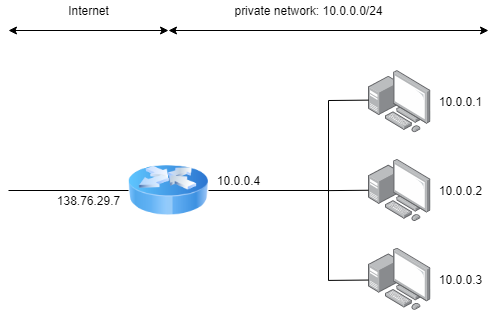
\includegraphics[width=300px]{images/5_Internetworking/NAT.png}
\end{figure}
La rete privata è 10.0.0.0/24, tra di loro gli host possono dialogare essendo nella stessa rete, per andare all' esterno serve qualcosa di più perché i loro indirizzi IP sono privati quindi il router si rifiuta di instradare pacchetti con quegli indirizzi IP.

Il NAT si occupa di sostituire l' IP sorgente privato con l' IP privato del router stesso, quindi quando 10.0.0.1 vuole dialogare con l' esterno invia datagrammi al router, il router sostituisce l' IP originale con 138.76.29.7 e provvede ad instradare il pacchetto sulla internet.

Per attuare questa traduzione il NAT usa una tabella interna di traduzione che associa all' indirizzo IP e porta del router esposta su internet l' indirizzo IP e porta dell' host interno alla rete.
Vediamo un esempio
\begin{itemize}
    \item 10.0.0.1 vuole trasmettere quindi crea un datagramma con 10.0.0.1:3345 e lo invia verso il router
    \item il router riceve il datagramma e sostituisce IP e porta con 138.76.29.7:5001 ed invia il datagramma verso internet.
    Inoltre aggiunge un record nella tabella in cui associa  138.76.29.7:5001 $<->$ 10.0.0.1:3345
    \item quando la rete risponde, risponde con un datagramma destinato a \\ 138.76.29.7:5001
    \item il router lo riceve, legge l' indirizzo IP, cerca nella sua tabella una entry con quell' indirizzo, la trova e traduce cambiando l' indirizzo IP in 10.0.0.1:3345 e provvede ad instradare il pacchetto nella rete locale.
\end{itemize}

Questo meccanismo come abbiamo visto funziona ed è molto elegante se è l' host interno alla rete a prendere l' iniziativa ed iniziare la comunicazione.
Se ad iniziare la comunicazione fosse un host nella Internet pubblica non potrebbe funzionare in quanto il NAT non è detto che abbia una entry che associ all' host interno alla rete.
Per risolvere questo problema si può ricorrere al port mapping cioè inserire manualmente delle righe nella tabella di traduzione in cui si associa una porta pubblica ad un host interno alla rete.
Questa tuttavia è una configurazione manuale permanente.

Un' altra soluzione è l' utilizzo dell'hole punching che non discuteremo.

Un' altra soluzione, utilizzata ad esempio da skype, è quella di passare per un host che è pubblico nella rete, detto relay, che mette in comunicazione i due host privati in maniera trasparente.

Questa traduzione fa uso delle porte del router, quindi abbiamo un limite massimo di oltre 60000 connessioni simultanee, che non è un grosso limite per le reti domestiche.
Un' altra controversia è quella che il router in mezzo, nonostante sia un dispositivo di layer 3, modifica informazioni del layer 4, quello di trasporto, quindi si sta violando la connessione end-to-end.
La soluzione migliore al problema sarebbe l' utilizzo di IPv6!

\subsection{Datagram forwarding}
\subsubsection{Forwarding nei router intermedi}
Se in una tabella di routing inserissimo singolarmente tutti gli host possibili avremmo una tabella troppo grande da poter gestire, la soluzione è memorizzare solamente gli indirizzi delle reti, dopodiché gli host nella stessa rete saranno tutti raggiungibili semplicemente instradando verso la sottorete.

Questa tabella quindi associa all' indirizzo di sottorete il prossimo hop al quale inoltrare il datagramma e l' interfaccia verso la quale si trova il next hop:
\begin{table}[ht!]
    \centering
    \begin{tabular}{l|l|l}
        Subnet Number & Next Hop & Interface \\
        \hline
        128.96.34.0/25 & Router R1 & interface 0 \\
        128.96.34.128/25 & Router R3 & interface 1 \\
        128.96.33.0/24 & Router R3 & interface 1 \\
    \end{tabular}
\end{table}

La codifica CIDR è comoda per noi umani che utilizziamo la notazione decimale, per i computer non lo è.
Nelle tabelle di forwarding quindi il CIDR viene memorizzato tramite una subnet mask che è un indirizzo scritto nella stessa notazione decimale puntata che però pone ad 1 i primi $x$ bit che compongono la porzione di rete.
Ad esempio una rete /24 ha la subnet mask 255.255.255.0, una /25 ha una subnet mask 255.255.255.128.

La tabella di forwarding è quindi meglio rappresentata da:
\begin{table}[ht!]
    \centering
    \begin{tabular}{l|l|l|l}
        Subnet Number & Subnet Mask & Next Hop & Interface \\
        \hline
        128.96.34.0 & 255.255.255.128 & Router R1 & interface 0 \\
        128.96.34.128 & 255.255.255.128 & Router R3 & interface 1 \\
        128.96.33.0 & 255.255.255.0 & Router R3 & interface 1 \\
    \end{tabular}
\end{table}

\begin{verbatim}
    DHost = Destination_IP_Address
    For each entry i in RoutingTable {
        DNet = (SubnetMask[i] & DHost)
        If(DNet == SubnetNumber[i]) {
            deliver datagram to NextHop[i] through Interface[i]
            break
        }
    }
\end{verbatim}

\subsubsection{Forwarding dall' host mittente}
Il mittente conosce il proprio indirizzo IP, la sua maschera di sottorete ed il suo default router, questo perché fa parte della configurazione di rete effettuata manualmente o tramite DHCP.
Se l' host deve inviare datagrammi ad un altro host e l' indirizzo IP destinatario è nella stessa rete allora lo invia direttamente, se l' IP destinatario è fuori dalla propria rete il datagramma è inviato verso il default router.
\begin{verbatim}
    SubnetNum = MySubnetMask & Dest_IP_Addr
    if(SubnetNum == MySubnetNum)
        deliver datagram to Dest_IP_Addr
    else
        forward datagram to default router
\end{verbatim}

\subsection{ARP}
Ogni volta che devo inoltrare un datagramma ad un qualsiasi host, che sia nella mia stessa rete o che sia fuori e quindi debba passare per il router, devo incapsulare il datagramma in un frame ethernet.
Per fare ciò devo conoscere l' indirizzo fisico dell' host destinatario o intermedio, ci serve quindi eseguire una traduzione degli indirizzi.
Il protocollo ARP - Address Resolution Protocol è utilizzato proprio per questo scopo.

L' host sorgente invia in broadcast una richiesta ARP contenente l' indirizzo IP del destinatario.
Essendo in broadcast tutti gli host della rete la ricevono, a questo punto il destinatario si accorge della richiesta e risponde con il proprio indirizzo fisico direttamente a chi gli ha fatto la richiesta, quindi non in broadcast.

Internamente agli host una cache mantiene le associazioni IP-MAC per un tempo ragionevole prima di cancellare l' associazione per evitare che l' informazione sia troppo vecchia e quindi obsoleta.

Questo protocollo è \emph{plug-and-play} in quanto non c'è bisogno dell'azione di nessuno affinché funzioni, è tutto automatico, nessuna configurazione da effettuare.

\subsection{ICMP}
Il protocollo ICMP - Internet Control Message Protocol è un protocollo usato da tutti gli host per inviare notifiche al livello di rete.
E' spesso utilizzato per notificare errori di qualche tipo al livello di rete, ma non solo.

Un messaggio ICMP si compone di:
\begin{itemize}
    \item un tipo
    \item un codice
    \item l' header ed i primi 8 byte di dati del datagramma IP che ha causato l' errore
\end{itemize}
Alcuni esempi sono:
\begin{table}[ht!]
    \centering
    \begin{tabular}{l|l|l}
        Tipo & Codice & Descrizione \\
        0 & 0 & Risposta all' echo \\
        3 & 0 & Rete di destinazione irragiungibile \\
        3 & 1 & Host di destinazione irragiungibile \\
        3 & 2 & Protocollo di destinazione non implementato \\
        3 & 3 & Porta di destinazione non aperta \\
        3 & 6 & Rete di destinazione sconosciuta \\
        3 & 7 & Host di destinazione sconosciuto \\
        8 & 0 & Richiesta echo \\
        9 & 0 & Router advertisement \\
        10 & 0 & Router discovery \\
        11 & 0 & TTL scaduto \\
        12 & 0 & Header IP errato \\
    \end{tabular}
\end{table}

NB: Il Router advertisement è la procedura effettuata dai router per dire alla rete che sono presenti e per spargere informazioni utili come ad esempio lo stato dei link ed il loro utilizzo.
Spesso queste informazioni sono utilizzate dagli altri router per costruire le proprie tabelle di routing o per aggiornare le proprie metriche.

NB: Il router discovery è il processo di ricerca dei router nelle vicinanze.

NB: I comandi ping e traceroute si basano sull' utilizzo di questo protocollo.

\subsection{IPv6}
Questa seconda versione del protocollo IP è stata creata per risolvere il problema della carenza degli indirizzi IP.
Inoltre ci sono altre motivazioni che spingono per il suo utilizzo come ad esempio:
\begin{itemize}
    \item il formato dell' header è pensato per rendere più veloce la processazione ed il forwarding dei datagrammi
    \item il formato dell' header è cambiato anche per facilitare la qualità del servizio
\end{itemize}
NB: IPv5 è un protocollo anch'esso - Internet Stream Protocol, per questo si ha il nome IPv6.

Il datagramma IPv6 prevede un header a dimensione fissa di 40 byte e non ammette la frammentazione.

\begin{figure}[H]
    \centering
    \includegraphics[width=200px]{images/5_Internetworking/IPv6_format.png}
\end{figure}
\begin{itemize}
    \item version: contiene sempre 6
    \item priority: indica la priorità del datagramma
    \item flow label: usato per identificare i datagrammi dello stesso flusso
    \item payload length: lunghezza in byte del campo dati
    \item next header: indica il protocollo del layer superiore
    \item hop limit: equivalente del TTL
\end{itemize}

NB: priority e flow label sono usati per gestire il QoS.

NB: non c'è un checksum per l' header, quindi non bisogna ricalcolarlo ogni volta che si decrementa hop limit.

Non essendoci frammentazione non possiamo inviare i datagrammi quando sono più grandi di MTU del media.
Questo significa che in caso ci sia questo problema si droppa del tutto il pacchetto e si invia un messaggio ICMP per notificare il mittente.
C'è anche una versione IPv6 di ICMP.

\subsubsection{Transizione da IPv4 ad IPv6}
Non essendoci la possibilità di passare da un giorno all' altro da un protocollo all' altro si sono applicate due soluzioni:
\begin{itemize}
    \item \emph{dual-stack}: i router implementano sia IPv4 che IPv6
    
    \item \emph{tunneling}: i datagrammi IPv6 vengono trasportati come dati all' interno di un datagramma IPv4 quando i router non possono dialogare nativamente IPv6:
    \begin{figure}[H]
        \centering
        \includegraphics[width=300px]{images/5_Internetworking/ipv6_tunnelling.png}
    \end{figure}
\end{itemize}

\section{Trasporto}
Il layer di rete si occupa di portare i dati da un host ad un altro host, ma il nostro scopo è trasportare dati da un processo ad un altro processo.

Il goal principale del layer trasporto è quindi il multiplexing/demultiplexing del flusso dei dati da e verso i vari processi.
Inoltre possiamo anche costruire meccanismi di trasferimento dati affidabile, controllo del flusso e controllo della congestione.

Abbiamo principalmente due protocolli TCP e UDP.

\subsection{Multiplexing \& Demultiplexing}
Il demultiplexing consiste nello smistamento del traffico in arrivo verso un host nei singoli processi che l' host ospita.
Questo può essere ottenuto tramite l' utilizzo del numero di porta, ogni processo che ha intenzione di comunicare tramite la rete è in ascolto su una porta, quando l' host riceve del traffico indirizzato su quella porta provvede ad inoltrarlo al singolo processo.

\subsubsection{Demultiplexing su servizio datagramma}
L' host riceve datagrammi IP, ogni datagramma contiene IP sorgente e destinatario, ogni datagramma trasporta un segmento del layer trasporto ed ogni segmento contiene la porta sorgente e la porta destinataria.

\subsubsection{Demultiplexing su servizio stream}
Il socket non è più qualcosa di indipendente, un singolo socket su un host è collegato al socket sull' altra macchina, quindi si crea una vera e propria connessione.
Questa connessione è identificata da IP e porta sorgente, IP e porta desinataria.
Durante la consegna si guardano quindi tutti questi parametri.
\begin{figure}[H]
    \centering
    \includegraphics[width=250px]{images/6_Trasporto/demux_with_multiprocess.png}
\end{figure}
Su una porta può essere in ascolto solo un processo, tuttavia se il processo forka, i figli ereditano tutti la stessa porta e quindi in questo caso si rende molto più importante il riconoscimento della informazione tramite questi 4 parametri.

\subsection{UDP}
E' uno dei primi protocolli standardizzati nella Internet moderna.
E' un servizio di tipo best-effort quindi possiamo perdere pacchetti o vederli consegnati fuori ordine.
Di fatto è assolutamente uguale a IP ma aggiunge il multiplexing ed il demultiplexing.

\subsubsection{Perché usarlo?}
Può tornare utile per il suo essere connectionless, essendo tale non c'è necessità di aprire una connessione quindi niente overhead.
E' estremamente semplice in quanto non mantiene uno stato né nella sorgente né nella destinazione.
Ci permette di avere più controllo sui dati in quanto non abbiamo controlli di flusso o di congestione.

E' largamente utilizzato per applicazioni loss tolerant o rate sensitive come lo streaming, ma anche in altri protocolli come DNS, NFS, SNMP ed il RIP (un protocollo di routing).

\subsubsection{Formato del segmento}
\begin{figure}[H]
    \centering
    \includegraphics[width=200px]{images/6_Trasporto/udp_segment.png}
\end{figure}

\begin{itemize}
    \item porta sorgente
    \item porta di destinazione
    \item lunghezza dei dati: lunghezza del segmento UDP inclusi gli header. Misurato in byte
    \item checksum
    \item dati
\end{itemize}
La checksum è utilizzata per eseguire una error detection, è eseguito tramite somma del contenuto in blocchi da 16 bit, se c'è un carry si somma al risultato, infine si fa il complemento ad 1.


\subsection{TCP}
Offre un servizio orientato alla connessione, quindi prima di trasmettere i dati c'è necessità di aprire una connessione, si usa il cosiddetto \emph{three-way handshake}.
Questa connessione è simile alla creazione del circuito virtuale, tuttavia i dispositivi del core non lo sanno, è qualcosa che riguarda solo gli host alle estremità del circuito.

Essendo un protocollo a flusso il pacchetto viene chiamato \emph{segmento}.
Implementa una connessione punto-punto quindi con un solo trasmettitore ed un solo ricevitore.
Questa connessione è full-duplex quindi entrambi gli endpoint possono inviare e ricevere allo stesso tempo.

Grazie a questo concetto di connessione possiamo costruire una trasmissione affidabile ed in ordine, si usano quindi dei buffer per inviare e ricevere.
Implementa un controllo del flusso quindi se il trasmettitore è troppo veloce il ricevitore glielo fa sapere ed il trasmettitore abbassa il suo rateo, questo si fa guardando la dimensione del buffer di ricezione e trasmettendolo al trasmettitore.

Invia i pacchetti in pipeline implementando un controllo di flusso e di congestione basato su finestra.

\subsubsection{Formato del segmento}
\begin{figure}[H]
    \centering
    \includegraphics[width=200px]{images/6_Trasporto/tcp_segment.png}
\end{figure}

\begin{itemize}
    \item porta sorgente
    \item porta destinataria
    \item numero di sequenza: usato per dare un ordine ai segmenti inviati, parte del meccanismo di in-order delivery.
    E' orientato al byte quindi al suo interno c'è la posizione nello stream del primo byte contenuto nel segmento
    \item numero di acknowledge: valido quando il bit di ACK è attivo, indica il numero di sequenza del prossimo pacchetto che si aspetta di ricevere
    \item head len
    \item NC
    \item flags:
    \begin{itemize}
        \item URG flag: poco usato
        \item ACK flag: indica che questo segmento è un acknowledge e quindi il campo di acknowledgement number è valido
        \item PSH flag: poco usato
        \item RST, SYN, FIN: usati per la connessione e la disconnessione.
    \end{itemize}
    \item receive window: il ricevitore vi scrive lo spazio libero nel proprio buffer di ricezione
    \item checksum
    \item urg data pointer: significativo solo se il flag URG è attivo, in genere poco usato
    \item opzioni: altre informazioni generalmente poco utilizzate
    \item payload
\end{itemize}

\subsubsection{Sequence number ed ACK}
\begin{figure}[H]
    \centering
    \includegraphics[width=150px]{images/6_Trasporto/sequence_number_ack.png}
\end{figure}
Il sequece number è il numero della posizione del primo byte del segmento dati nello stream.
L' ACK è il numero di sequenza del prossimo segmento che l' host si aspetta di ricevere.

L' inoltro out-of-order è gestito in maniera differente in base alle implementazioni, non c'è uno standard.

\subsubsection{Allocazione della connessione}
La fase di creazione della connessione è la fase in cui vengono allocate tutte le strutture dati necessarie per la gestione di questo meccanismo.
Da parte del client avviene quando si usa la primitiva connect(...) su un socket TCP (SOCK\_STREAM su AF\_INET).
Da parte del server avviene quando si usa la primitiva accept(...) su un socket TCP.

\subsubsection{Three-way handshake}
\begin{figure}[H]
    \centering
    \includegraphics[width=150px]{images/6_Trasporto/threeway_handshake.png}
\end{figure}

\begin{itemize}
    \item il client invia un segmento con il flag SYN attivo, senza dati e con un sequence number iniziale generato casualmente

    \item il server riceve il segmento con il flag SYN attivo e risponde con un segmento con SYN ed ACK attivo.
    Inserisce nessun dato e specifica un sequence number generato casualmente, mentre inserisce come acknowledge number il valore del sequence ricevuto incrementato di 1.
    In questa fase il server alloca i buffer.

    \item il client riceve il segmento con SYN-ACK  e risponde con un segmento con solo ACK attivo.
    Inoltre inserisce anche l'acknowledge number come segment number ricevuto incrementato di 1.
    A questo punto potrebbe già inviare dei dati.
\end{itemize}
Si creano dei sequence number casuali per evitare che il client si connetta, chiuda subito la connessione, poi la riapra subito dopo ed allora nei buffer interni vi rimangano ancora i dati vecchi.

\subsubsection{Connection tear-down}
\begin{figure}[H]
    \centering
    \includegraphics[width=200px]{images/6_Trasporto/connection_teardown.png}
\end{figure}

\begin{itemize}
    \item il client invia un pacchetto con il flag FIN attivo
    \item Il server lo riceve e risponde con un segmento con il flag ACK attivo, invia i dati che deve ancora inviare, chiude la connessione ed infine invia un pacchetto con FIN.
    \item il client una volta ricevuto il pacchetto di FIN risponde con un pacchetto ACK.
    Durante questo tempo il server rimane ancora in attesa di ricevere l' ACK
\end{itemize}
Se l' ACK del FIN del server non arriva o il FIN del server si perde (che sono la stessa cosa) il server provvede a re-inviare nuovamente il FIN.
Quindi sia il client che il server rimangono in attesa di avere questa conferma della chiusura della connessione.

\subsubsection{Reliable data transfer}
Il TCP crea un servizio di trasmissione affidabile usando il canale costruito da IP.
Sfrutta uno schema di tipo ARQ: Acknowledgements, Retransmissions and Timeouts basato su finestra.

L' intervallo di timeout è qualcosa che non è possibile calcolare perché dipende fortemente dal ritardo di accodamento, questo ritardo tuttavia si verifica su ogni router che si incontra quindi è casuale.
Conviene fare una stima basata sul RTT degli ultimi pacchetti inviati e la ricezione dei loro ACK.
Il primo segmento lo inviamo con un intervallo di timeout abbastanza grande e fisso, i successivi intervalli invece li calcoliamo tramite una media esponenziale mobile:
$$ ERTT_1 = RTT_0 $$
$$ ERTT_2 = \alpha \cdot RTT_1 + (1-\alpha) \cdot RTT_0 $$
$$ ERTT_3 = \alpha \cdot RTT_2 + \alpha(1-\alpha) \cdot RTT_1 + (1 - \alpha)^2 \cdot RTT_0 $$
$$ ERTT_{n+1} = \alpha \cdot RTT_n + (1 - \alpha) \cdot ERTT_n $$

\begin{itemize}
    \item RTT: round trip time misurato
    \item ERTT: estimated round trip time. $0 < \alpha < 1$
\end{itemize}

NB: $\alpha \approx 0$: da molto peso alla storia passata e poco a quella recente.

$\alpha \approx 1$: da molto peso alla storia recente e poco a quella passata.
Dopo numerose simulazioni sul campo si misura che il valore ottimale è $\alpha = 0.125$.

Ora abbiamo il valore stimato di RTT, dobbiamo trasformarlo in un intervallo di tempo da aspettare, possiamo fare diverse scelte:
\begin{itemize}
    \item secondo l' algoritmo di Karn-Partridge dovremmo usare come intervallo di tempo $2 \cdot ERTT$.
    In questo caso i pacchetti che sono stati ritrasmessi perché persi non vengono aggiunti alla stima di ERTT.
    
    \item secondo l' algoritmo di Van Jacobson - Karel si usa la stima di ERTT con aggiunta di un margine di sicurezza calcolato come: $DevRTT_{n+1} = (1-\beta)\cdot DevRTT_n + \beta\cdot|RTT_n - ERTT_n|$.
    Infine l' intervallo lo si fa di dimensione $ERTT + 4 \cdot DevRTT$.
    Tipicamente $\beta=0.25$
\end{itemize}

\subsubsection{TCP semplificato}
Vediamo come funziona una versione del TCP che ignora gli ACK duplicati, la gestione del flusso e della congestione.

Il trasmettitore come eventi può:
\begin{itemize}
    \item ricevere dati dall' applicazione: in questo caso bisogna creare un segmento con il numero di sequenza opportuno, una volta inviato bisogna far partire il timer (che è riferito sempre al pacchetto più vecchio, quindi parte se già non ce n'è uno attivo, altrimenti non ne parte uno nuovo)
    
    \item segnalazione del timeout: in questo caso si ritrasmettono i segmenti che hanno causato il timeout e si fa ripartire il timer
    
    \item ricezione di un ACK: in questo caso se l'ACK è di pacchetti non precedentemente confermati si aggiorna l' elenco dei pacchetti non confermati e si sposta il timer in modo da far riferimento al primo pacchetto non confermato.
\end{itemize}

\begin{verbatim}
// Sender
NextSeqNum = InitialSeqNum
SendBase = InitialSeqNum

while(1){
    switch event {
    case DATA_RCVD:
        packet = make_segment(NextSeqNum, data)
        if !timer:
            timer.start()
        send_data_to_network(packet)
        NextSeqNum += length(data)
    break;
    
    case TIMEOUT:
        for p in window:
            send_data_to_network(p)
        timer.start()
    break;
    
    case ACK:
        if y > SendBase:
            SendBase = y
            if NextSeqNum != SendBase:
                timer.start()
    break;
    }
}    
\end{verbatim}

Scenari di ritrasmissione:
\begin{itemize}
    \item ci perdiamo l'ACK, aspettiamo il timeout e reinviamo il segmento

    \item inseriamo il timeout troppo presto quindi ritrasmettiamo i segmenti e poco dopo ci arriva l' ACK precedente, in questo caso avremo degli ACK duplicati

    \item se inviamo più segmenti, ci perdiamo l' ACK del primo ma riceviamo quelli successivi possiamo leggerlo come ACK cumulativo e quindi non ritrasmettiamo perché diamo per scontato che il ricevitore abbia ricevuto anche quelli precedenti e che abbiamo perso l' ACK
\end{itemize}
Ogni volta che eseguiamo una ritrasmissione raddoppiamo l' intervallo di timeout (exponential increase), è una tecnica di controllo della congestione.

\subsubsection{Fast retransmission}
Il periodo di timeout spesso è troppo lungo da aspettare quindi potrebbe succedere di dover aspettare la scadenza del timer pur sapendo che alcuni pacchetti sono stati persi.
Questo può succedere quando si ricevono ACK duplicati, aggiungiamo quindi la politica che se riceviamo 3 ACK duplicati (cioè 4 ACK per lo stesso segmento) procediamo a ritrasmettere senza aspettare che il timeout scada.
\begin{figure}[H]
    \centering
    \includegraphics[width=200px]{images/6_Trasporto/fast_retransmit.png}
\end{figure}

NB: Il protocollo TCP non è propriamente né Go-Back-N né Selective Repeat, è un ibrido in quanto ritrasmette dal primo segmento non ACK (quindi non N segmenti indietro) ma non prevede l'ACKnowledge dei singoli segmenti.

\subsubsection{Sommario degli eventi}
Gli eventi del ricevitore sono quindi:
\begin{itemize}
    \item arrivo di un segmento in ordine con numero di segmento aspettato, con tutti i segmenti fino a quel punto ACKati.
    Si aspettano 500ms prima di inviare l'ACK per vedere se è in arrivo qualche altro segmento in modo da eseguire un ACK cumulativo, se non arriva si procede ad inviare l' ACK.

    \item arrivo di un segmento in ordine con un numero di segmento aspettato ma con almeno un altro segmento non ACKato.
    Si invia immediatamente un ACK cumulativo in modo da confermare tutti e due i segmenti.

    \item arrivo di un segmento out-of-order con numero di segmento più grande di quello aspettato, si ha un gap.
    Si invia immediatamente un ACK duplicato indicando il sequence number del segmento che si sta aspettando.
    
    \item arrivo di un segmento che riempie un gap completamente o parzialmente.
    Si invia immediatamente un ACK se il segmento ricevuto si trova all' inizio del gap.
\end{itemize}

\subsubsection{TCP Flow Control}
Il ricevitore ha un buffer di ricezione, è pertanto necessario implementare un meccanismo di controllo del flusso per evitare che il ricevitore sia inondato di dati dal trasmettitore.

Dobbiamo innanzitutto capire come calcolare lo spazio libero rimanente nel buffer di ricezione: il protocollo mantiene come informazioni:\\ per il trasmettitore:
\begin{itemize}
    \item la dimensione totale del buffer
    \item l' indice dell' ultimo byte ACKato (LastByteAcked)
    \item l' indice dell' ultimo byte inviato (LtByteSent)
\end{itemize}
per il ricevitore:
\begin{itemize}
    \item la dimensione totale del buffer
    \item l' indice dell'eventuale buco mancante in caso di ricezione out-of-order (NextByteExpected)
    \item l' indice dell' ultimo byte ricevuto (LastByteRcvd)
\end{itemize}
Definiamo che se ci sono dei buchi dovuto alla consegna out-of-order comunque quello non è spazio libero perché a breve sarà colmato e comunque non possiamo metterci altri dati perché sono riservati ai byte in ordine.
La dimensione totale occupata è quindi $LastByteRcvd - LastByteRead$, la dimensione dello spazio libero è pertanto $DimensioneBuffer - SpazioOccupato$.

Il ricevitore dunque ad ogni ACK inserisce nel campo receive window la dimensione dello spazio libero in modo da rendere conscio il trasmettitore di quanto ancora possa inviare.

Se il ricevitore risponde dicendo che ha spazio libero 0 il trasmettitore provvede periodicamente ad inviare segmenti di dimensione 1 in modo da stimolare una risposta dal destinatario ed essere aggiornato sull' evolvere della situazione.

\begin{figure}[H]
    \centering
    \includegraphics[width=200px]{images/6_Trasporto/free_space_calculation.png}
\end{figure}

\subsection{Controllo della congestione}
La congestione consiste nell' avere troppe sorgenti che inviano troppi dati troppo velocemente affinché la rete possa gestire tutto ciò.
Quando questo succede si ha perdita di pacchetti e delay lunghi perché le code si riempono.
Succede sui router intermedi che devono smistare il traffico.

A differenza del controllo di flusso, che riguarda sorgente e destinazione, il controllo della congestione riguarda i nodi intermedi della rete.

Possiamo avere due approcci risolutivi alla congestione:
\begin{itemize}
    \item Network-assisted: i router intermedi forniscono feedback agli host, possiamo segnalare singolarmente la congestione oppure dire esplicitamente a quale rateo inviare i pacchetti
    
    \item End-to-end: niente feedback dalla rete, si inferisce la congestione quando si hanno rallentamenti e perdita di pacchetti.
    Questo approccio conservativo è utilizzato dal TCP.
\end{itemize}


\subsubsection{Congestion control network assisted in ATM}
Il protocollo ATM mette a disposizione una classe di servizio con garanzia del troughput minimo detta ABR (available bit rate), questa classe di servizio deve implementare un meccanismo di controllo della congestione affinché possa garantire la banda minima.

Uno dei meccanismi che si possono utilizzare a tale scopo è RM cells: la sorgente tra i vari pacchetti di dati ne invia alcuni detti RM cells (resource management) con dei bit che possono essere settati dagli switch incontrati durante il percorso, questi bit sono:
\begin{itemize}
    \item NI bit: (no increase in rate) indica che c'è una leggera congestione e si dovrebbe evitare di aumentare il rate per non cadere nella congestione completa

    \item CI bit: (congestion indication) che indica che siamo effettivamente in una congestione e quindi sarebbe ottimale diminuire il rate
    
    \item byte ER: (explicit rate) il mittente inserisce all' interno il suo rateo corrente, ogni switch sul percorso può abbassarlo solamente in modo da indicare la velocità massima da tenere in caso di congestione
\end{itemize}
questi pacchetti inviati dal sender verso il receiver vengono poi rispediti dal ricevitore al sender con i bit modificati, possibilmente.
\begin{figure}[H]
    \centering
    \includegraphics[width=330px]{images/6_Trasporto/ATM_ABR_congestion_control.png}
\end{figure}
Nelle celle di dati vi è anche il bit EFCI che viene settato ad 1 dagli switch congestionati, se la cella dato che precede una cella RM ha il bit EFCI settato il mittente setta il bit CI nelle celle RM che vengono rispedite indietro.


\subsubsection{Congestion control end-to-end in TCP}
L' obiettivo è far si che tutte le sorgenti possano trasmettere il più velocemente possibile senza che la rete si congestioni.

Per limitare il rate di trasmissione possiamo inviare meno byte nella stessa finestra di tempo, per fare questo abbassiamo il numero di segmenti non ackati nella pipeline ad un valore che chiameremo \verb{cwnd{ (congestion window) che rispetta:
$$ LastByteSent - LastByteAcked \leq cwnd $$

Questo valore in realtà viene scelto come il minimo tra la dimensione della congestion windows e la dimensione della receiver window, facendo così possiamo abbassare il rateo di pacchetti inviati.
Si noti che cwnd è dinamico e dipende dal livello di congestione della rete.

Per accorgersi di una congestione della rete il protocollo TCP si basa sugli ACK e sui segmenti perduti.
Se ho ottenuto ACK allora la rete non è congestionata e posso aumentare il rate, se ho dei segmenti persi invece assumo che la perdita sia dovuta alla congestione della rete e quindi abbasso il rateo di invio.
I paccheti persi sono sentiti tramite il time-out o 3 ACK duplicati.

L' idea di base dietro all' algoritmo è di fare \emph{probing} della bandwith:
\begin{itemize}
    \item quando ricevo degli ACK incremento il rateo di trasmissione (aumento di una quantità fissa)

    \item quando invece si hanno delle perdite si diminuisce il rate
\end{itemize}
L' andamento del rate è tipicamente a dente di sega perché segue questi aumenti e queste decrescite.

Dividiamo il protocollo in 3 fasi:
\begin{itemize}
    \item Slow start: aumentare linearmente la dimensione della finestra all' inizio è controproducente in quanto devo massimizzare il rateo il prima possibile, alla partenza abbiamo quindi come \verb{cwnd{ 1MSS (maximum segment size) e come rate MSS/RTT ed incrementiamo raddoppiando il rateo ad ogni ACK finché non superiamo un particolare threshold o non otteniamo una perdita di pacchetti.
    Una volta superato la threshold si va in fase congestion avoidance.
    
    Di default il threshold è 64Kbyte.

    \item Congestion avoidance: si incrementa linearmente cwnd ad ogni ACK.
    Quando si hanno 3 ACK duplicati modifichiamo:
    $$ threshold = \frac{cwnd}{2} $$
    $$ cwnd = \frac{cwnd}{2} + 3 \cdot MSS $$
    e si va in fast recovery.

    Quando si ha un timeout invece:
    $$ threshold = \frac{cwnd}{2} $$
    $$ cwnd = 1 $$
    e si torna in slow start.

    \item Fast recovery: 
    
\end{itemize}
\begin{figure}[H]
    \centering
    \includegraphics[width=250px]{images/6_Trasporto/TCP_congestion_control_FSM.png}
\end{figure}

Si noti che il TCP assume che qualsiasi packet loss sia dovuto alla congestione, questa assunzione non è vera nei casi in cui si usino dei link con perdite come i link wireless o le reti con nodi mobili.
Questo purtroppo porta ad abbassare il rateo anche quando non sarebbe strettamente necessario, è quindi consigliato implementare delle notifiche esplicite sulla congestione.

Il protocollo TCP è fair quindi se $K$ sessioni TCP condividono lo stesso bottleneck $R$ allora ogni sessione finirà ad avere rateo medio di $\frac{R}{K}$.
Vediamo una simulazione:
\begin{figure}[H]
    \centering
    \includegraphics[width=200px]{images/6_Trasporto/TCP_fairness.png}
\end{figure}
Inizialmente si parte da uno scompenso tra le due connessioni, entrambe crescono linearmente perché in fase di congestion avoidance, appena la somma dei throughput supera la capacità del canale si avranno delle perdite di pacchetti o ACK triplicati quindi il protocollo vedrà questi eventi come una congestione e dimezzeranno il throughput, eseguendo questa procedura abbastanza volte si finisce a convergere sulla linea di bandwith uguale.




\section{Security}
\subsection{Pericoli della rete}
I protocolli di rete sono intrinsecamente non sicuri in quanto sono stati pensati in un periodo in cui la sicurezza non era qualcosa di importante.
Per questo motivo possono essere eseguiti alcuni attacchi ai vari protocolli.

\subsubsection{Packet sniffing}
Le trasmissioni su media in broadcast come ethernet o wireless sono soggetti a packet sniffing cioè un utente malevole è capace di catturare tutto il traffico in transito e carpire le informazioni comunicate tra i due endpoint della comunicazione.

\subsubsection{IP spoofing}
Non essendoci autenticazione sull' indirizzo IP un host può forgiare pacchetti con indirizzi IP sorgente diversi dal proprio e fingersi questo secondo host.

\subsubsection{Denial of Service}
Un folto gruppo di utenti organizzato può saturare di traffico un server e farlo collassare, in questo modo il server non può più fornire il suo servizio, è una negazione di servizio.
Di solito l' attacco è distribuito: Distributed Denial of Service ed il gruppo sorgente dell' attacco è detto \emph{botnet}.

\subsubsection{Replay attack}
Essendo il traffico in chiaro molto spesso possiamo pensare di catturare porzioni del traffico e re-inoltrarlo così com'è a piacere.

\subsubsection{Malware}
Si potrebbe usare la rete per iniettare codice malevolo all' interno degli hosts.
Tra questi malware possiamo annoverare gli spyware che si occupano di registrare la tastiera, i siti visitati e tante altre informazioni sull' utente.
Possiamo pensare di arruolare gli host in una botnet per portare avanti attacchi DDoS.

\subsection{Come proteggersi?}
La prima forma di protezione è la consapevolezza, eseguire programmi arbitrari scaricati dalla rete potrebbe essere dannoso ad esempio.

Gli aspetti di interesse per una comunicazione sono:
\begin{itemize}
    \item confidenzialità: solo il mittente ed il destinatario scelto dovrebbero poter comprendere il contenuto del messaggio.
    
    \item autenticazione: il mittente ed il destinatario vogliono essere certi di star parlando l' uno con l' altro e non con qualcuno che si spaccia come tale
    
    \item integrità: il mitente ed il destinatario vogliono essere sicuri che il messaggio non venga alterato durante la trasmissione
    
    \item accesso e disponibilità: il servizio proposto deve essere accessibile e disponibile
\end{itemize}
per alcuni scopi sono importanti solo alcune caratteristiche, per altri tutte quante.

\subsection{Crittografia}
Per ottenere tutte o alcune di queste proprietà possiamo usare la crittografia!
Più genericamente possibile la crittografia si occupa di prendere un messaggio \emph{in chiaro} e di restituirne un altro in forma cifrata utilizzando un algoritmo di cifratura ed una chiave.
Per gli utilizzi comuni l' algoritmo è noto a tutti e pubblico mentre le chiave (o le chiavi) sono note solo agli endpoint della comunicazione.
Diremo:
\begin{itemize}
    \item $m$ testo in chiaro
    \item $K_A(m)$ testo cifrato con algoritmo $K$ e chiave $A$
    \item $m = K_B(K_A(m))$ applicando l' algoritmo di decifrazione con la chiave di decifratura sul messaggio cifrato si riottiene il messaggio in chiaro
\end{itemize}

Possiamo discernere gli algoritmi crittografici in varie classi in base allo schema che si utilizza.

\subsubsection{Crittografia simmetrica}
La chiave di cifratura e la chiave di decifratura sono identiche, è un segreto condiviso.
Prima di potersi scambiare dei messccaaggi occorre quindi mettersi d' accordo sulla chiave comune da utilizzare.

\subsubsection{Cifrario di Cesare}
Un esempio di cifrario simmetrico è il cifrario di Cesare, si tratta di un cifrario a sostituzione che sostituisce ad ogni lettera la lettera che lo segue ad una distanza $k$.
Possiamo pertanto costruire una tabella di corrispondenza che sostituisce ad ogni lettera un' altra e per cifrare non ci basta che scorrere questa tabella di corrispondenza mentre per decriptare si scorre la tabella nel senso contrario.

La chiave in questo schema crittografico è il numero di shift da eseguire.

\subsubsection{Sostituzione monoalfabetica}
E' la versione generale del cifrario di Cesare che associa una sostituzione arbitraria.
In questo caso la chiave è la tabella che associa l' alfabeto originale alla sua versione cifrata.

\subsubsection{Sostituzione polialfabetica}
In questo metodo anziché cifrare una lettera sempre con la stessa si scelgono varie tabelle di sostituzione monoalfabetica e si usano tutte seguendo un determinato pattern.
Con questo algoritmo lo spazio delle chiavi è estremamente elevato e difficilmente attaccabile tramite altri metodi.

\subsubsection{Crittografia simmetrica moderna}
La crittografia simmetrica moderna si divide in due macro categorie:
\begin{itemize}
    \item cifrari a flusso: cifra un bit per volta
    \item cifrario a blocco: cifra singoli blocchi di plaintext e cifra ognuno di essi singolarmente
\end{itemize}

Per misurare la sicurezza di un algoritmo di misura il tempo ipoteticamente necessario a romperlo con qualsiasi metodo.

\subsubsection{DES - Data Encryption Standard}
E' uno dei primi cifrari a blocchi che prevede chiavi di 56 bit, il DES è poco sicuro e pertanto poco utilizzato odiernamente in quanto si rompe facilmente tramite una ricerca esaustiva ed altri tipi di attacchi.

Una versione più sicura costruita sulla base del DES è il triplo DES che usa tre chiavi differenti ed esegue in sequenza: encryption, decryption ed encryption.
Anche questa versione tuttavia soffre di alcune lacune.

\subsubsection{AES - Advanced Encryption Standard}
L' algoritmo crittografico più usato oggi è l' AES che prevede chiavi a 128, 192 o 256 bit.

\subsubsection{Scambio delle chiavi}
La crittografia simmetrica ha un grande problema: lo scambio delle chiavi.
Essendo uguale per entrambi gli endpoint la chiave non può essere inviata in chiaro sul canale di comunicazione perché potrebbe venire carpita e quindi utilizzata per decriptare anche dagli estranei.

Un metodo sarebbe quello dello scambio diretto in persona ma non sempre i due endpoint possono incontrarsi per scambiarsi la chiave di persona.

Possiamo usare come rifermento un centro di distribuzione delle chiavi ma dovrebbe essere una entità certificata ed affidabile per entrambi i partecipanti.

Possiamo utilizzare la crittografia a chiave pubblica, che è il metodo moderno.

\subsubsection{Crittografia a chiave pubblica}
In questo schema crittografico ogni utente ha una coppia di chiavi:
\begin{itemize}
    \item chiave privata: conosciuta solo al possessore
    \item chiave pubblica: generata a partira dalla chiave privata e resa pubblica per tutti
\end{itemize}

Per inviare un messaggio si prende il plaintext e lo si cifra con la chiave pubblica del destinatario, per decifrare è necessario ricorrere alla chiave privata del destinatario, essendo privata e nota solo a lui si ha la confidenzialità delle informazioni, inoltre non dobbiamo effettuare uno scambio delle chiavi in quanto quella pubblica è nota a tutti.

\subsubsection{RSA}
L' algoritmo di crittografia asimmetrica più conosciuto è quello RSA (Rivest, Shamir, Adleman) che gode di una importante proprietà: applicare prima la chiave pubblica e poi quella privata è equivalente ad applicare prima quella privata e poi quella pubblica.

\subsubsection{Chiavi di sessione}
Dal momento che gli algoritmi asimmetrici sono molto meno efficienti in termini computazionali li usiamo per scambiare una chiave e successivamente la vera e propria comunicazione avviene mediante crittografia simmetrica.
La chiave che ci si scambia è unica per ogni sessione di comunicazione, quindi la chiave prende il nome di \emph{chiave di sessione}.

\subsection{Integrità ed autenticazione}
Permette ai partecipanti della comunicazione di verificare che il messaggio ricevuto è autentico.
Inoltre l' integrità garantisce:
\begin{itemize}
    \item che la sorgente sia chi penso che sia
    \item che il contenuto del messaggio non venga alterato
    \item che il messaggio non possa essere replicato
    \item che la sequenza dei messaggi sia mantenuta correttamente
\end{itemize}

\subsubsection{Message Digest}
Un digest di un messaggio è il risultato di una funzione hash con ingresso il messaggio stesso.
Chiamiamo il digest $H(m)$.

Alcune proprietà importanti di queste funzione sono:
\begin{itemize}
    \item facile da calcolare
    \item difficile da invertire (irreversibile)
    \item deve restituire un messaggio di lunghezza fissa partendo da messaggi di lunghezza arbitraria
    \item resistente alle collisioni, cioè deve essere difficile trovare due input che ci danno lo stesso output
    \item deve produrre un output che sembri randomico
\end{itemize}

\subsubsection{Message Authentication Code - MAC}
Preso un messaggio ed un segreto condiviso eseguiamo l' hash della concatenazione dei due, questo valore lo inviamo assieme al messaggio stesso.
Chi riceve il messaggio per accertarsi che sia autenticato deve solamente eseguire nuovamente l' algoritmo di hashing sul messaggio ed il segreto condiviso, se è identico al MAC ricevuto allora il messaggio non è stato modificato.

\begin{figure}[H]
    \centering
    \includegraphics[width=300px]{images/7_Security/Message_authentication_code.png}
\end{figure}

Questo metodo funziona se il segreto è conosciuto solo ed esclusivamente dai due endpoint della comunicazione.

Oltre a provare l' integrità del messaggio il MAC funge anche da autenticazione in quanto il segreto è noto solo alle due controparti.

L' algoritmo HMAC è una versione di MAC standardizzata che usa gli algoritmi di hash MD5 e SHA-1:
\begin{itemize}
    \item concatenare segreto e messaggio
    \item hashare la concatenazione
    \item concatenare l' hash ottenuto al messaggio
    \item hashare la nuova concatenazione
\end{itemize}

\subsubsection{Esempio con OSPF - Open Shortest Path First}
OSPF è un algoritmo di routing quindi permette l' advertising delle route.
Si potrebbe quindi pensare di fingersi un router ed inviare pacchetti forgiati a piacere, oppure cancellare pacchetti in modo che non arrivino a destinazione o addirittura modificarli.
Ci serve un meccanismo di autenticazione dei messaggi, OSPF mette a disposizione 3 metodi:
\begin{itemize}
    \item nessuna autenticazione
    \item password condivisa tra tutti i nodi che però viene inserita in chiaro in un campo del pacchetto OSPF
    \item autenticazione con hash crittografico: si fa un hash del pacchetto OSPF e della chiave segreta condivisa, quindi si concatena al pacchetto OSPF
\end{itemize}

\subsubsection{Firma digitale}
E' un meccanismo crittografico analogo alla firma cartacea:
\begin{itemize}
    \item verificabile: chi riceve il messaggio può verificare che il mittente sia chi effettivamente dice di essere
    
    \item non forgiabile: il mittente può e solo lui può effettuare la firma
    
    \item non ripudiabilità: il ricevente può provare che il mittente ha firmato un messaggio e non un altro
    
    \item integrità del messaggio: il mittente può provare che ha firmato un messaggio e non un altro
\end{itemize}
Il MAC non può essere utilizzato come firma digitale in quanto il segreto è conosciuto da almeno due enti quindi ognuno dei due potrebbe firmare a nome dell' altro, vengono meno la verificabilità, la non forgiabilità e la non ripudiabilità.

La firma digitale deve quindi essere creata usando la crittografia a chiave pubblica: il mittente cifra il messaggio con la sua chiave privata e gli altri usano la sua chiave pubblica per decifrarlo.
Se la chiave privata è effettivamente privata allora solo un utente può forgiare i messaggi, quindi è verificabile.

Abbiamo tuttavia detto che cifrare con la crittografia a chiave pubblica è dispendioso e non si può fare per messaggi troppo lunghi, la soluzione è quindi firmare un hash del messaggio e non il messaggio stesso:
\begin{itemize}
    \item Il mittente invia la concatenazione del messaggio con la firma dell' hash del messaggio
    
    \item Il destinatario per autenticare il messaggio deve eseguire l' hash del messaggio e confrontare che sia uguale all' hash decifrato con la chiave pubblica
\end{itemize}

\begin{figure}[H]
    \centering
    \includegraphics[width=330px]{images/7_Security/signed_MAC.png}
\end{figure}

Tutta questa teoria si basa sull' assunto che la chiave pubblica che si utilizza per verificare sia effettivamente la chiave pubblica associata alla chiave privata usata per firmare, questo assunto non sempre è vero, l' attaccante potrebbe ad esempio aver intercettato e sostituito la chiave pubblica durante la trasmissione tra i due che comunicano.

\subsubsection{Certification of authority}
E' un ente che collega le chiavi pubbliche agli utenti attraverso un certificato.
Chi depone la propria chiave pubblica deve fornire documentazione in modo che la CA si accerti dell' identità, la CA crea il certificato inserendo all' interno le informazioni circa l' utente e lo firma con la propria chiave privata.

Quando un utente vuole la chiave pubblica di un altro utente la chiede alla CA, gli viene fornito un certificato che può controllare tramite la chiave pubblica della CA.
Ogni CA a sua volta è certificata da un' altra authority in uno schema ad albero alla radice del quale c'è un organo ritenuto affidabile.

\subsubsection{Certificato}
E' un documento digitale che contiene la chiave pubblica assieme alle informazioni del proprietario della chiave pubblica.
Viene inoltre firmato dall' autorità che lo rilascia.

Ha un formato standardizzato in RFC 2459.

\subsubsection{Attacchi playback}
Supponiamo di eseguire un pagamento e di chiedere alla nostra banca di effettuarlo, seppure il messaggio è criptato possiamo registrarlo e reinviarlo a piacere per ri-eseguire questa transazione.

Per risolvere questo problema nel messaggio di transazione si embedda un valore casuale che cambia ad ogni messaggio, la stessa banca ci dice di utilizzare questo determinato valore quindi se andiamo ad eseguire altre richieste, essendo cambiato questo valore, non possiamo utilizzare messaggi pre-registrati.

\begin{figure}[H]
    \centering
    \includegraphics[width=100px]{images/7_Security/nonce_usage.png}
\end{figure}

\subsection{Mettere in sicurezza le email}
Per mettere in sicurezza le email dovrei ottenere:
\begin{itemize}
    \item confidenzialità
    \item autenticazione del mittente
    \item autenticazione del destinatario
    \item integrità del messaggio
\end{itemize}

Un primo schema che garantisca confidenzialità ed integrità prevede la cifratura del messaggio con un algoritmo simmetrico, la chiave utilizzata invece la si cifra con la chiave pubblica del destinatario.
Il destinatario non deve fare altro che decriptare la chiave simmetrica utilizzando la propria chiave privata e decriptare il messaggio cifrato con la chiave segreta ottenuta.

Per ottenere l' autenticazione nello schema possiamo aggiungere al messaggio un hash del messaggio firmato con la chiave privata del mittente, il destinatario deve quindi eseguire l' hash del messaggio ricevuto e confrontarlo con il risultato della decifratura dell' hash ricevuto.

\subsubsection{PGP - Pretty Good Privacy}
E' una suite software che prevede algoritmi simmetrici ed asimmetrici, funzioni hash ed algoritmi di firma digitale.
E' lo standard de-facto per lo scambio di email in sicurezza.
NB: il creatore Phil Zimmerman è stato indagato per 3 anni dopo aver reso pubblico questo software.

\subsection{SSL (Secure Socket Layer) e TCP/IP}
SSL è un protocollo che viene posizionato tra il livello di trasporto ed il livello di applicazione, si tratta di un middleware quindi.
Mette a disposizione del programmatore delle API per fornire crittografia a livello applicazione senza preoccuparsi della implementazione ma pensando solo alla logica dell' applicazione.

Permette di ottenere confidenzialità, integrità dei dati ed autenticazione degli endpoint, gli obiettivi principali per i quali è stato creato sono la messa in sicurezza delle transazioni negli e-commerce, cifratura dei dati ed autenticazione del web server.
Si può anche utilizzare per autenticare i client ma spesso non si fa.

La versione più aggiornata è nota come TLS ed è descritta in RFC 2246.
Per utilizzarla si deve scrivere le proprie applicazioni utilizzando i secure socket anziché quelli normali.

Una versione semplificata di SSL lavora tramite:
\begin{itemize}
    \item Handshake
    \item Key derivation
    \item Data transfer
    \item Connection Closure
\end{itemize}

\subsubsection{Handshake}
I due endpoint usano i propri certificati e le proprie chiavi private per autenticarsi a vicenda e scambiarsi un segreto condiviso:
\begin{figure}[H]
    \centering
    \includegraphics[width=100px]{images/7_Security/ssl_handshake.png}
\end{figure}

\subsubsection{Key derivation}
I due endpoint usano lo shared secret per derivare un insieme di chiavi di sessione:
\begin{itemize}
    \item $K_c$ chiave per criptare i dati dal client verso il server
    \item $M_c$ chiave per generare il MAC dal client al server
    \item $K_s$ chiave per criptare dati dal server al client
    \item $M_s$ chiave per generare il MAC dal server al client
\end{itemize}
le chiavi vengono prodotte utilizzando un algoritmo di derivazione delle chiavi.

\subsubsection{Data Transfer}
I dati da trasferire sono suddivisi in una serie di blocchi detti \emph{record}, ogni blocco ha un MAC posizionato alla fine del record.
Per permettere record di diversa lunghezza e comunque poter discernere tra dati e MAC si inserisce un campo lunghezza all' inizio.

Per impedire attacchi di record \& playback si inserisce nei record un numero di sequenza usato per computare il MAC, in questo modo anche replicando il record il MAC computato sarà diverso e quindi il record verrà droppato.

Per evitare truncation attacks, cioè una terminazione improvvisa della connessione, si usa un campo di \emph{tipo}, anch' esso usato nel calcolo del MAC.

\subsubsection{Record SSL}
La struttura di un record è:
\begin{figure}[H]
    \centering
    \includegraphics[width=200px]{images/7_Security/ssl_record.png}
\end{figure}
$$ MAC = MAC(M_x, sequence||type||data) $$

\subsubsection{Connection closure}
Si usano messaggi speciali per chiudere la connessione per evitare alcuni problemi che potrebbero venire a crearsi.

\subsubsection{SSL completo}
Al protocollo che abbiamo pensato mancano alcune cose come la negoziazione della cipher suite: i due endpoint devono mettersi d' accordo su quali algoritmi utilizzare quindi devono scambiarsi l' elenco degli algoritmi che effettivamente conoscono.
Una cipher suite deve contenere:
\begin{itemize}
    \item un algoritmo a chiave pubblica
    \item un algoritmo simmetrico
    \item un algoritmo per il calcolo del MAC
\end{itemize}

Nel protocollo SSL completo durante l' handshake si deve quindi:
\begin{itemize}
    \item autenticare il server
    \item negoziare una cipher suite che sia implementata in entrambi gli endpoint della comunicazione
    \item stabilire delle chiavi
    \item autenticare il client (non obbligatoriamente)
\end{itemize}

La negoziazione della cipher suite avviene come segue:
\begin{enumerate}
    \item il client invia al server la lista completa degli algoritmi che può supportare, insieme ad un nonce

    \item il server sceglie da questa lista di algoritmi e li comunica al client assieme al proprio certificato ed un secondo nonce
    
    \item il client verifica il certificato, ne estrae la chiave pubblica, genera un pre-master-secret e lo cifra con la chiave pubblica del server, glielo comunica
    
    \item client e server costruiscono indipendentemente le chiavi a partire dal pre-master-secret
    
    \item il client invia il MAC di tutto l' handshake
    
    \item il server invia il MAC di tutto l' handshake
\end{enumerate}
Gli utlimi due passaggi prevengono l' handshake dal tampering in quanto un attacco man-in-the-middle potrebbe modificare la lista degli algoritmi del client eliminando gli algoritmi forti e lasciando solo quelli deboli.

I nonce inviati dal client e dal server sono utilizzati per evitare attacchi reply in quanto: se io prendo tutti i messaggi del client e provo a reinviarli fingendomi lui, il server mi risponderà con un nonce diverso da quello della prima volta quindi le chiavi crittografiche cambieranno e l' attacco non potrà essere portato avanti.

\subsection{VPN e IPsec}
Le Virtual Private Network permettono di creare delle reti completamente separate dall' internet pubblica sfruttando l' internet pubblico stesso.
Creare una rete separata da internet sarebbe molto dispendioso perché richiederebbe una intera infrastruttura di rete a parte, invece possiamo sfruttare la rete che già esiste: il traffico interno ad una rete aziendale lo spediamo attraverso la Internet pubblica ma lo inviamo criptato.

Una implementazione delle VPN si ottiene utilizzando il protocollo IPsec, implementato sui router o sui singoli host che si occupa di prendere i datagrammi IP, rimpiazzare il payload con un header IPsec ed il payload criptato.
Ovviamente alla ricezione bisogna prendere l' header IPsec ed il payload criptato e svolgere le azioni al contrario.

Questo protocollo permette l' integrità dei dati, autenticazione della sorgente, previene gli attacchi di tipo replay e provvede alla confidenzialità dei dati.
Questo servizio può essere fornito attraverso due protocolli:
\begin{itemize}
    \item Authentication header (AH): fornisce l' autenticazione della sorgente e l' integrità dei dati, ma non la confidenzialità
    \item Encapsulation Security Protocol (ESP): fornisce autenticazione della sorgente, integrità dei dati e confidenzialità
\end{itemize}
Parleremo di ESP.

Qualsiasi VPN prevede, prima di inviare qualsiasi dato, la creazione di una connessione virtuale tra le due entità della comunicazione, questa connessione viene chiamata \emph{Security Association}, queste sono simplex quindi permettono ad un host di parlare e ad un altro di ascoltare, quindi se ci sono $N$ nodi che vogliono partecipare alla rete ci vogliono $2 + 2N$ security association (contando anche quelle del quartier generale).

Entrambi i nodi della comunicazione mantengono informazioni sugli stati della connessione (quindi rendono IP un protocollo connection-oriented):
\begin{itemize}
    \item security parameter index: stringa da 32 bit che individua la SA che l' host sta gestendo
    \item IP della interfaccia di origine
    \item IP della interfaccia di destinazione
    \item tipo di cifratura utilizzato
    \item chiave di cifratura
    \item tipo del controllo di integrità (HMAC, ecc)
    \item chiave di autenticazione (segreto per il MAC)
\end{itemize}
Tutte queste informazioni sono all' interno del Security Association Database (SAD).

Un datagramma IPsec che utilizza il protocollo ESP è costituito:
\begin{figure}[H]
    \centering
    \includegraphics[width=330px]{images/7_Security/IPsec_datagram.png}
\end{figure}
NB: il padding nel trailer serve per rendere il contenuto un multiplo intero del blocco affinché si possano usare gli algoritmi di crittografia a blocchi.

Così facendo abbiamo eseguito una encapsulation del vecchio datagramma IP in uno nuovo ma con il payload criptato.

Come fa un router a sapere quali datagrammi deve incapsulare e quali no?
All' interno del router si trova un Security Policy Database (SPD) che dato un datagramma ne controlla IP sorgente e destinatario ed il numero di protocollo ed in base a questi dati cerca nella sua tabella interna se usare IPsec ed in tal caso quale security association utilizzare.

\subsection{Firewalls}
E' un dispositivo hardware o software che si utilizza per isolare la rete interna dall' Internet permettendo solo ad alcuni pacchetti di entrare e/o uscire bloccando tutti gli altri.

\subsubsection{Perché?}
Permette di mitigare attacchi di tipo DoS perché ci permette di isolare quegli host che generano tanto traffico o richieste SYN che poi non vengono concluse.
Previene modifiche ed accessi illeciti a dati interni alla rete.
Permette l' accesso alla rete solo ad elementi autorizzati.

\subsubsection{Tipologie}
Riconosciamo tre tipologie di firewall:
\begin{itemize}
    \item stateless packet filters
    \item stateful packet filters
    \item application gateways
\end{itemize}

\subsubsection{Stateless packet filtering}
Il router applica dei filtri sui singoli pacchetti decidendo se fare forward o dropparli in base a:
\begin{itemize}
    \item IP sorgente e destinazione
    \item porta sorgente e destinazione
    \item messaggi ICMP
    \item i flag dei pacchetti TCP
\end{itemize}

Queste regole vengono indicate compilando delle apposite \emph{Access Control List} che indicano l' azione da intraprendere sul filtro selezionato.
Le regole si leggono dall' alto verso il basso, la prima che matcha il pacchetto che si sta elaborando viene eseguita.
Alla fine si inserisce una \emph{deny all} oppure una \emph{allow all}, ovviamente si consiglia di utilizzare una deny all in quanto è una opzione più sicura.

Esempio di ACL:
\begin{table}[ht!]
    \centering
    \begin{tabular}{c|c|c|c|c|c|c}
        action & \thead{source \\ address} & \thead{dest \\ address} & protocol & \thead{source \\ port} & \thead{dest \\ port} & \thead{flag \\ bit}  \\
        \hline
        allow & 222.22/16 & \thead{outside of \\ 222.22/16} & TCP & $>$1023 & 80 & any \\ 
        allow & \thead{outside of \\ 222.22/16} & 222.22/16 & TCP & 80 & $>$1023 & ACK \\
        allow & 222.22/16 & \thead{outside of \\ 222.22/16} & UDP & $>$1023 & 53 & --- \\
        allow & \thead{outside of \\ 222.22/16} & 222.22/16 & UDP & 53 & $>$1023 & --- \\ 
        deny & all & all & all & all & all & all \\ 
    \end{tabular}
\end{table}

\subsubsection{Stateful packet filtering}
Permette il filtering dei pacchetti con coscienza del loro stato all' interno della comunicazione.
Traccia l' inizio e la fine della connessione TCP in modo da sapere se i pacchetti in transito hanno senso, inoltre applica dei timeout alle connessioni in modo da droppare i pacchetti di connessioni scadute.

Anche in questo caso si utilizzano delle ACL con però le opzioni per tracciare lo stato come ad esempio i bit flaggati.

Esempio di ACL:
\begin{table}[ht!]
    \centering
    \begin{tabular}{c|c|c|c|c|c|c|c}
        action & \thead{source \\ address} & \thead{dest \\ address} & proto & \thead{source \\ port} & \thead{dest \\ port} & \thead{flag \\ bit} & \thead{check \\ conxion} \\
        \hline
        allow & 222.22/16 & \thead{outside of \\ 222.22/16} & TCP & $>$1023 & 80 & any & \\
        allow & \thead{outside of \\ 222.22/16} & 222.22/16 & TCP & 80 & $>$1023 & ACK & $\times$ \\
        allow & 222.22/16 & \thead{outside of \\ 222.22/16} & UDP & $>$1023 & 53 & --- & \\
        allow & \thead{outside of \\ 222.22/16} & 222.22/16 & UDP & 53 & $>$1023 & --- & $\times$ \\ 
        deny & all & all & all & all & all & all & \\ 
    \end{tabular}
\end{table}

\subsubsection{Application gateways}
Permette di applicare filtri ai dati così come ai campi IP e TCP/UDP, per esempio possiamo permette ad un utente interno alla rete di collegarsi in telnet all' esterno.
Si tratta di una macchina specifica adibita a ricevere determinato traffico e si occupa di spedirlo all' esterno, internamente ad una rete solo lui ha il permesso di inviare questo traffico quindi fa da middleware per tutti gli altri host.

Un esempio è un web proxy usato per filtrare in base ai domini o alle categorie.

\subsubsection{Limitazioni di firewall ed application gateway}
Se volessimo usare tante applicazioni che necessitano di un trattamento specifico dovremmo configurare un application gateway per ognuno di loro, questo comporta che il client che vuole usare quel software debba esserne a conoscenza e debba essere configurato per utilizzarlo.

Inoltre non eliminano tutte le possibili minacce: un utente malintenzionato interno alla rete o esterno ad essa potrebbe modificare l' IP sorgente di alcuni pacchetti eseguendo il così detto IP spoofing, in tal caso il router e gli eventuali firewall ed application gateway non possono essere certi della provenienza dei pacchetti.

\subsubsection{Intrusion Detection Systems}
Il normale packet filtering lavora esclusivamente sugli header TCP ed IP non eseguendo alcuna correlazione tra le varie sessioni.
Gli IDS invece possono eseguire una deep packet inspection, possono cioè guardare il contenuto dei pacchetti, ed anche esaminare correlazioni tra più pacchetti.
Sono capaci di accorgersi di eventuali port scanning, network mapping ed attacchi DoS.

Solitamente se ne inseriscono diversi nella rete in modo da segmentare la rete applicando diversi controlli sul traffico.

\section{Wireless and Mobile Network}
Fino ad ora abbiamo trattato le reti con il presupposto che i nodi siano fermi nello spazio, negli ultimi anni tuttavia abbiamo assistito ad una vera e propria rivoluzione mobile.
La maggior parte degli host oggi giorno sono mobili, a partire dai dispositivi connessi tramite Wi-Fi, passando per quelli connessi a rete mobile di un qualche operatore telefonico, finendo per i cosidetti dispositivi IoT.
Si parla quindi di \emph{ubiquitous computing} cioè sistemi pervasivi talmente presenti da non farci neanche caso.

\subsection{Caratteristiche dei canali wireless}
Abbiamo diverse tecnologie wireless da quelle a corto raggio a quelle a lungo raggio, alcune caratteristiche sono:
\begin{itemize}
    \item la perdita di potenza del segnale: i segnali radio perdono potenza con almeno il quadrato della distanza

    \item interferenze da altre sorgenti: i collegamenti wireless sono molto più soggetti ad interferenze esterne e ci sono molte più sorgenti di interferenza
    
    \item multipath propagation: la propagazione del segnale può seguire diversi percorsi quindi un ricevitore riceve segnali uguali in tempi diversi, sfasati, bisogna quindi trovare il modo di non leggere un segnale arrivato tardi come un nuovo segnale
\end{itemize}
quello che ci interessa, dal punto di vista delle reti, è il bit error rate, questo dipende dalla codifica che decidiamo di utilizzare, non ce n'è una migliore in quanto ne esistono di veloci che però hanno un error rate alto e viceversa ne esistono di stabili ma lente.
I sistemi quindi sono di tipo adattativo cioè cambiano codifica in base alle condizioni del mezzo.

Il canale wireless è inoltre broadcast quindi è molto semplice che un host causi delle collisioni. Ci sono delle soluzioni a questo problema ma ne abbiamo alcuni altri.

\subsubsection{Problema del nodo nascosto}
Supponiamo di avere 3 ricetrasmettori: A, B e C e che:
\begin{itemize}
    \item A comunichi con B e viceversa
    \item B comunichi con C e viceversa
    \item A e C non possono comunicare perché hanno un ostacolo tra di loro oppure perché sono troppo distanti e l' attenuazione è troppa
\end{itemize}
quello che potrebbe succedere è che A e C comunicano allo stesso tempo, B riceve entrambi i segnali, c'è una collisione ma se ne accorge solamente B.
Pur facendo carrier sense A e C non possono sapere che c'è stata una collisione e non possono quindi attuare politiche di mitigazione.
\begin{figure}[H]
    \centering
    \includegraphics[width=250px]{images/8_Wireless_Mobile/wireless_attenuation.png}
\end{figure}

\subsubsection{Classificazione delle reti wireless}
Possiamo classificare le reti wireless in base alle dimensioni:
\begin{itemize}
    \item BAN: Body Area Network: pensate per reti di sensori indossabili, sotto il metro
    \item PAN: Private Area Network: pensate per piccoli dispositivi wireless con portata di qualche metro, ad esempio mouse, tastiere e dispositivi bluetooth
    \item WLAN: wireless LAN, le normali aree wireless per i computer
    \item Reti cellulari: reti GSM, GPRS, UMTS, LTE, ecc
\end{itemize}

Oppure in base alle infrastrutture:
\begin{itemize}
    \item reti basate su una infrastruttura: reti mobili.

    \item reti senza infrastruttura ad hoc: ad esempio reti formate da dispositivi bluetooth o le reti utilizzare da organi di pronto intervento che non possono fare affidamento su reti già esistenti.
    I nodi possono essere statici o mobili, possono essere multi-hop, possono poi essere connesse a delle reti pre-esistenti, ecc, ecc.

    \item reti ibride: reti con una porzione dotata di infrastruttura dedicata ed una porzione senza.
\end{itemize}

\subsection{Wireless LAN - 802.11}
E' lo standard de-facto per le reti wireless LAN meglio conosciute come Wi-Fi.
E' uno standard IEEE che ne raggruppa varie versioni in base alle frequenze ed altre caratteristiche.

E' un tipo di rete con infrastruttura, abbiamo quindi l' infrastruttura di rete fissa alla quale si aggiunge un \emph{Access Point} cioè una base station che si occupa di dialogare con i client wireless.
L' area di copertura è detta \emph{Basic Service Set} (oppure hotspot o cella).

Ogni host deve quindi associarsi ad un access point, spesso potrebbe ricevere il segnale di più di uno di essi e deve quidi scegliere quale usare.
Due access point adiacenti devono lavorare su canali diversi, cioè su frequenze di trasmissione diverse, ce ne sono 11 che occupano l' intero spettro che va dai 2.4GHz ai 2.485GHz.

\subsubsection{Associazione dell' host}
Quando un host vuole connettersi sceglie un canale e si mette in ascolto, esegue così la scansione di tutti i vari canali.
Gli Access Point ogni 100 ms inviano un beacon cioè un segnale che dice in broadcast il nome dell' access point (detto SSID) ed il suo indirizzo MAC.

Quindi l' host sceglie l' AP al quale associarsi, esegue eventualmente l' autenticazione necessaria, successivamente si configura in automatico con DHCP o in maniera statica ed è pronto a navigare.

\subsubsection{Accesso al mezzo}
Essendo il mezzo condiviso tra tutti c'è bisogno di un protocollo di accesso, potremmo pensare di utilizzare CSMA/CD tuttavia in questo ambiente non può essere utilizzato perché:
\begin{itemize}
    \item il dispositivo wifi se sta trasmettendo non può ascoltare il mezzo perché dotato di una sola antenna. Potremmo risolvere usando due antenne

    \item il problema del nodo nascosto persiste e non ci permette di detectare collisioni in quanto accadono sul nodo intermedio, non su chi sta trasmettendo.
\end{itemize}

Si usa un nuovo protocollo detto CSMA/CA (Collision avoidance) che si occupa di prevenire le collisioni, che tuttavia possono comunque accadere ancora.
Usiamo uno schema ARQ con una divisione in slot molto piccoli usati solo per dare il punto di inizio delle operazioni:
\begin{figure}[H]
    \centering
    \includegraphics[width=300px]{images/8_Wireless_Mobile/802.11_comunication.png}
\end{figure}
\begin{enumerate}
    \item la sorgente vuole inviare un frame, il mezzo deve essere libero per un certo tempo che chiamiamo DIFS.

    \item se c'è stato DIFS tempo libero allora invia il frame

    \item subito dopo la ricezione del frame il destinatario muta da ricevitore a trasmettitore, questo tempo è detto SIFS (switching time) e deve essere necessariamente minore di DIFS.

    \item a questo punto il destinatario invia un ACK del pacchetto
\end{enumerate}
NB: SIFS $<$ DIFS perché altrimenti un altra stazione potrebbe inserisi nel mezzo ed inviare un frame causando una collisione.

Questa prima versione non tiene conto del fatto che potrebbero esserci più nodi in attesa di inviare: supponiamo ci siano due nodi che vogliono inviare, entrambi ascoltano il mezzo e misurano DIFS tempo libero, quindi trasmettono.
In questo scenario abbiamo certamente una collisione!
Per risolvere introduciamo un backoff time, ogni stazione oltre ad aspettare DIFS time ne aspetta altro randomicamente in modo da sparpagliare i tentativi.

Se mentre il timer di backoff ci si accorge che un' altra stazione inizia a trasmttere si congela il proprio timer e lo si risveglia dopo la fine della trasmissione e l' attesa del nuovo periodo DIFS.

Come tempo di backoff si sceglie un numero random di slot da aspettare in [0, CW-1].
Inizialmente CW vale cwim (standard del protocollo), quando si ha un ACK mancante si raddoppia CW fino ad arrivare a CWmax.

Questo protocollo tuttavia non ci risolve il problema del nodo nascosto: se i due nodi che vogliono comunicare non si vedono tra di loro ognuno vedrà il canale libero ed andrà a trasmettere causando una collisione in ricezione sull' access point.

Un altro problema che c'è è quello del nodo esposto: supponiamo di avere 4 nodi che parlano a due a due: B parla con A e C parla con D, D riesce a vedere solamente C.
Se B inizia a trasmettere verso A la stazione C non potrà trasmettere verso D in quanto troverà il canale occupato.
Se C non seguisse il protocollo e comunque trasmettesse potrebbe anche non causare problemi in quanto magari A è molto lontano da C, in questo caso si ha addirittura una perdita di tempo nell' attesa del canale libero.

E' stato quindi sviluppato un meccanismo detto \emph{virtual carrier sensing} che si contrappone al physical sensing perché anziché controllare la potenza del segnale per vedere l' utilizzazione del mezzo si esegue una specie di prenotazione del mezzo:
\begin{figure}[H]
    \centering
    \includegraphics[width=330px]{images/8_Wireless_Mobile/virtual_carrier_sensing.png}
\end{figure}
Supponiamo ci sia una stazione che voglia trasmettere, allora guarda il canale e vede se è libero per un tempo DIFS, a quel punto invia un pacchetto RTS (request to send), viene ricevuto sia dalla stazione base che da tutte le altre stazioni vicini alla sorgente, chiunque senta questo pacchetto imposta un timer (NAV RTS - network allocation vector RTS) con la durata specificata nel campo \emph{duration} in RTS.
Successivamente dopo un tempo SIFS la base station risponde con un pacchetto CTS (clear to send) che contiene anche lui il campo \emph{duration}, con contenuto minore di quello trasferito dalla sorgente, ed è usato per far partire il timer (NAV CTS) a tutti gli altri nodi che non avevano sentito prima RTS.
Quando la sorgente percepisce il CTS (fa da acknowledge alla richiesta di trasmissione) aspetta un tempo SIFS ed inizia a trasmettere il frame.
Dopo la completa trasmissione del frame la stazione base attende un tempo SIFS ed invia un pacchetto di ACK.
Tutti gli altri nodi quindi vedono l' ACK e dopo un tempo DIFS fanno partire un timer di backoff con valore caricato randomicamente.

NB: se due host inviano RTS allo stesso tempo c'è ancora una collisione, tuttavia la grandezza di RTS è molto piccola quindi le probabilità di trasmissioni simultanee sono molto piccole ed anche se succedesse avremmo solo perso il tempo dell' invio di RTS.

NB: nonostante abbiamo risolto il problema c'è un aumento dell' overhead in quanto tutto il tempo dello scambio di RTS e CTS è tempo in cui non inviamo dati.
Per questi ed altri motivi se la grandezza del frame è paragonabile a quella di RTS/CTS non si esegue questo protocollo ma si invia direttamente il frame.

\subsubsection{Struttura del frame}
\begin{figure}[H]
    \centering
    \includegraphics[width=330px]{images/8_Wireless_Mobile/802.11_frame.png}
\end{figure}
\begin{itemize}
    \item frame control: contiene informazioni di controllo sul frame
    \item duration: usato nei frame RTS e CTS per far settare i NAV alle altre stazioni
    \item address 1: indirizzo MAC della stazione che deve ricevere il frame
    \item address 2: indirizzo MAC della stazione che sta trasmettendo il frame
    \item address 3: indirizzo MAC dell' interfaccia del router al quale l' access point è collegato.
    E' utilizzato per trasformare il frame WiFi in un frame ethernet, questa traduzione è effettuata dall' access point che funziona un po' come un bridge.
    
    \item sequence control: numero di sequenza utilizzato per la ritrasmissione e l' acknowledge
    \item address 4: usato solo nella modalità ad hoc (quando una stazione comunica con un' altra senza l' ausilio di una stazione base)
    \item payload: i dati veri e propri
    \item CRC
\end{itemize}
il campo frame control a sua volta è costituito da:
\begin{figure}[H]
    \centering
    \includegraphics[width=330px]{images/8_Wireless_Mobile/802.11_frame_control.png}
\end{figure}
\begin{itemize}
    \item protocol version
    \item type: RTS, CTS, ACK, Data
    \item subtype
    \item to AP: indica se il frame è diretto all' access point
    \item from AP: indica se il frame è proveniente dall' access point
\end{itemize}

\subsubsection{Mobilità nella stessa rete}
Con le reti wireless possiamo avere problemi di mobilità, cioè l' utente si sposta.
Se la mobilità è nell' hotspot dell' access point allora non c'è nessuna modifica del funzionamento.

Se invece l' utente si sposta abbastanza da dover cambiare access point, ma comunque sempre nella stessa sotto rete, i due access point si mettono d'accordo e c'è una procedura di sgancio da uno ed aggancio all' altro.
Lo switch al quale gli access point sono associati potrebbe non capire che c'è stato un campio di topologia, quindi finché la tabella ARP non viene flushata l' host non riceverà i frame, dato che però il flush avviene molto spesso questo non è un problema.

\subsubsection{Power managment}
Essendo ora i dispostivi mobili è normale che vengano alimentati tramite batterie, quindi sarebbe bello prevedere all' interno dei protocolli di trasmissione dei metodi per risparmiare energia elettrica.
L' access point emette dei beacon ogni 100ms, come abbiamo già detto, sia per la discovery delle stazioni, sia per sincronizzare il clock, sia per le politiche di power management.

Quello che si fa è che i nodi vanno in sleep ed avvisano l' access point, a questo punto quando l' access point riceve frame che dovrebbero andare ad un nodo in sleep li mantiene in memoria ed aspetta che il nodo si risvegli prima di inoltrarli a lui.
Quando il nodo si risveglia ed effettua la sincronizzazione tramite il beacon con l' access point esso ne approfitta inviando la lista dei frame in coda.

C'è un piccolo delay quindi (sleep delay) perché bisogna aspettare che il nodo si risvegli, tuttavia c'è un grande guadagno in termini di energia preservata, si può ottenere fino al 90\% di efficienza.

\subsection{Architettura della rete mobile cellulare}
Questa rete è composta da alcune centraline che gestiscono un insieme di stazioni radio base.
Ogni smartphone si registra ad una stazione radio base e quindi si registra ad un centralino che poi è connesso alla rete intenet pubblica.

In origine la rete cellulare era una vera e propria rete telefonica tuttavia ormai anche la rete telefonica è stata convertita in una rete a commutazione di pacchetto.
Ogni stazione radio base viene detta cella quindi si parla appunto di reti cellulari.

NB: la forma esagonale è usata perché si disegna meglio, kek, in realtà sarebbero circolari.

Anche la rete cellulare essendo wireless è un mezzo broadcast quindi è necessario utilizzare protocolli che evitino le collisioni.
Per risolvere questi conflitti spesso si usano combinazioni di TDMA, FDMA e spread spectrum.

\subsubsection{Generazioni della tecnologia}
Ci sono diverse generazioni di questa rete cellulare, la prima era completamente analogica.

La seconda generazione, 2G, detta anche GSM combinava FDMA e TDMA era pensato solo per la voce ma era completamente digitale.
E' stata poi anche usata per trasmettere dati esattamente come si faceva con i modem casalinghi che sfruttavano la rete telefonica.

La seconda generazione e mezza, 2.5G, detta anche GPRS era una evoluzione del 2G che sfruttava sempre la stessa rete ma prendeva alcuni slot e li utilizzava esculsivamente per il traffico dati, rendendone più economico l' utilizzo.

La terza generazione, 3G, detta anche UTMS integra voci, video e dati in una singola rete.

La quarta generazione, 4G, detta anche LTE è completamente una rete IP sia per la trasmissione dei dati che per la trasmissione della voce.

La quinta generazione, 5G, pensata per applicazioni real time e mobili, quindi bassa latenza e pervasività.

\subsection{Mobilità in internet}
Internet è stata pensata per nodi stazionari e link affidabili (e wired), tuttavia l' evoluzione che ha preso non è stata questa.
Per alcuni versi la mobilità può essere gestita con soluzioni esistenti come il DHCP, tuttavia ci sono alcuni casi in cui questa gestione non basta per garantire la continuità del servizio.

\subsubsection{Mobilità per IP}
Dal punto di vista di IP la mobilità può essere:
\begin{itemize}
    \item nessuna: un host cambia punto di accesso alla rete ma rimane sempre nella stessa sottorete.
    Ad esempio un utente che cambia access point.
    In questo caso per il protocollo IP non ho cambiato punto di accesso, sono sempre nella stessa sottorete

    \item media: un host cambia rete acquisendo un nuovo indirizzo IP tramite il DHCP.
    Questa è mobilità ma senza continuità, non c'è da preoccuparsene

    \item alta: un utente si sposta da una rete all' altra in poco tempo, si ha ad esempio quando si viaggia ed il dispositio aggancia diverse reti man mano che ci si sposta.
    La continuità con la quale avvengono questi cambiamenti portano ad una situazione problematica e quindi è necessaria la gestione
\end{itemize}

Se per mantenere la continuità nel caso della mobilità alta dovessi disconnettermi e riconnettermi ogni volta che cambio indirizzo IP avrei un servizio intermittente.
Una gestione di questo caso non è previsto da IP, servono altre procedure ed altri protocolli.

\subsubsection{Indirect routing}
Una soluzione derivante da scenari del mondo reale prevede l' utilizzo di un \emph{home agent} che lavori per conto dell' host mobile.
Vediamo una situazione tipica:
\begin{figure}
    \centering
    \includegraphics[width=250px]{images/8_Wireless_Mobile/mobility.png}
\end{figure}
supponiamo che l'host si trovi sempre nella home network ma a volte si sposti nella visited network, le due reti sono reti diverse con indirizzamenti diversi.
Chiamiamo il router della home network \emph{home agent} mentre chiamiamo il router della visited network \emph{foreign agent}.
Potremmo risolvere il problema attraverso i protocolli di routing annunciando che l' host si è spostato, tuttavia non è fattibile perché il routing funziona sulla base della rete e non del singolo host.

E' necessario che a gestire questa situazione siano direttamente gli host: quando l' host mobile arriva nella rete visitata, contatta il foreign agent e gli dice di registrarlo presso l' home agent.
Il foreign agent quindi contatta l' home agent avvisandolo che se dovessero arrivare dei pacchetti indirizzati verso l' host esso dovrà rispedirli al foreign agent perché l' host si è spostato.

L' host che quindi è all' altro endpoint della connessione (correspondent) non sa niente di questo cambiamento, continua e continuerà a spedire pacchetti a quello stesso indirizzo.
Quando l' host deve rispondere al correspondent invece può farlo direttamente.

Questo approccio funziona tuttavia c'è questa triangolazione del traffico che spesso è inutile e potrebbe essere evitabile, prende il nome di: triangolo del routing.
Questa soluzione è detta anche \emph{routing indiretto}:
\begin{figure}[H]
    \centering
    \includegraphics[width=250px]{images/8_Wireless_Mobile/indirect_routing.png}
\end{figure}
NB: l' home agent ed il foreign agent possono essere i router delle reti in cui l' host decide di spostarsi tuttavia non è obbligatorio.

NB: l' indirizzo IP orginale viene detto \emph{permanent address} mentre quello nuovo assunto una volta cambiata la rete viene detto \emph{care-of-address}.

Questo metodo è completamente trasparente al correspondent che non verrà mai a sapere che l' host si è spostato.

Si noti che se l' host si spostasse nuovamente esso dovrà nuovamente eseguire la registrazione presso l' home agent, in questo periodo la connessione non è presente, se quindi l' host è molto mobile si rischia di impiegare più tempo nel processo di registrazione che nella vera e propria navigazione.

\subsubsection{Direct routing}
Per risolvere il problema della triangolazione potremmo usare la tecnica del direct routing cioè quando il correspondent invia il datagramma all' home agent esso gli fa sapere che l' host si è spostato e gli indica anche dove.
In questo modo il correspondent può virare il suo traffico direttamente verso il foreign agent presso il quale si trova l' host mobile:
\begin{figure}[H]
    \centering
    \includegraphics[width=250px]{images/8_Wireless_Mobile/direct_routing.png}
\end{figure}

Abbiamo eliminato la triangolazione del routing ma questo nuovo metodo non è trasparente rispetto al correspondent.
Se l' host mobile si sposta nuovamente in un' altra rete il correspondent continuerebbe ad inviare i datagrammi alla prima rete visitata, quindi è necessario che al nuovo spostamento l' host mobile si registri verso il vecchio foreign agent in modo che il correspondent possa essere avvisato del nuovo spostamento e dirotti ancora una volta il traffico verso la nuova posizione.

Per chi ha invece iniziato la connessione prima del secondo spostamento si ha una chain dei diversi foreign agent.

\subsubsection{Mobile IP}
E' un protocollo che usa l' approccio del routing indiretto, è descritto in RFC 3344 ed aggiunge il meccanismo di agent discovering e delle metodologie di registrazione verso l' home agent.

Quando l' home agent riceve un datagramma che deve instradare verso la nuova locazione dell' host mobile lo incapsula in un nuovo datagramma IP (inserendo come protocollo di layer superiore sempre IP, questo fa sì che questa incapsulazione possa essere eliminata all' arrivo senza particolari modifiche) e lo instrada.
Passa verso i foreign agent e viene recapitato all' host mobile.

L' agent discovery viene eseguito attraverso datagrammi ICMP trasmessi in broadcast dal foreign/home agent ad intervalli regolari:
\begin{figure}[H]
    \centering
    \includegraphics[width=330px]{images/8_Wireless_Mobile/agent_discovery.png}
\end{figure}
il pacchetto ICMP è di tipo 9 ed aggiunge dei campi specifici per gli utilizzi di discovery:
\begin{itemize}
    \item bit H/F: usati per indicare se è un home agent e/o un foreign agent
    \item bit R: indica se è necessaria la registrazione
\end{itemize}

La registrazione consiste di 4 passi: supponendo che l' host mobile sia arrivato nella nuova rete e che abbia correttamente ottenuto un indirizzo IP, allora
\begin{itemize}
    \item l' host mobile aspetta di ricevere un pacchetto ICMP per l' agent discovery, in questo pacchetto ci sono dei care-of-address offerti, ne sceglie uno e se lo assegna

    \item invia un messaggio al foreign agent in cui trasmettere:
    \begin{itemize}
        \item COA: care-of-address scelto
        \item HA: indirizzo dell' home agent
        \item MA: suo indirizzo corrente
        \item lifetime
        \item identificativo usato come numero di sequenza
    \end{itemize}
    
    \item il foreign agent riceve la richiesta di registrazione, memorizza i dati ivi contenuti e spedisce la richiesta all' home agent aggiungendo anche una nota sul tipo di encapsulation da usare.
    
    \item l' home agent riceve questa registrazione, segna le informazioni, abbassa il lifetime richiesto e risponde con un pacchetto di risposta identico a quello di registrazione ma togliendo il COA
    
    \item il foreign agent ottiene la risposta dall' home agent e la spedisce all' host mobile. Da questo momento in poi l' eventuale correspondent può inviare traffico e verrà instradato verso il mobile host.
\end{itemize}

\subsection{Effetti della mobilità sui protocolli di alto livello}
Logicamente l' impatto dovrebbe essere minimo tuttavia data la natura di TCP, che vede nella perdita di pacchetti una congestione, si ha una forte diminuzione della performance.
Questo è vero anche se si ha a che fare con collegamenti wireless o in genere con collegamenti che possono avere delle perdite.

Quello che si fa per non perdere performance nel caso delle reti wireless è gestire la perdita di pacchetti a livelli più bassi quindi tramite schemi ARQ prima di far arrivare i dati al layer TCP.

Un' altra opzione è quella di rendere noto al layer TCP la causa della perdita di pacchetti in modo che non abbassi il rate di trasmissione.
Possiamo anche pensare ad una connessione splittata, cioè due connessioni: una convenzionale in TCP su media cablato ed un' altra su media wireless che non deve necessariamente utilizzare TCP puro.

Queste modifiche alla fine non sono state molto utilizzate in quanto i media wireless sono aumentati in affidabilità.


\subsection{Infrastructure-less (Ad hoc) networks}
Sono reti composte esclusivamente da dispositivi dotati di antenna senza l' utilizzo di una infrastruttura alle spalle.

\subsubsection{WPAN Bluetooth}
Un esempio di queste reti è la rete Bluetooth, non ci sono infrastrutture alle spalle, la rete è composta esclusivamente dagli endpoint della rete.
Il bluetooth è un metodo di trasmissione a short range su 2.4GHz, è low-cost ed utilizza poca energia.
Pensato inizialmente per il cable replacement (ad esempio mouse, tastiere e stampanti bluetooth), per la comunicazione telefonica in ambito locale (cordless, auricolari bluetooth e comunicazioni in bluetooth tra dispositivi vicini) ora l' utilizzo principale è quello di costituire delle reti ad hoc per lo scambio di dati.

Lo standard delle reti bluetooth è detto Piconet, si compone di un master e di tanti slave, il master è quello che decide di creare la rete, gli slave sono quelli che decidono di aggiungersi ala rete.

Permette di utilizzare 78 frequenze portanti tra i 2.4GHz ed i 2.4835 GHz in contemporanea utilizzando il frequence hopping: si opera su una frequenza per un certo time slot, alla fine si passa sul prossimo e così via.
Questa coordinazione è eseguita attraverso il master e tutti sono messi a conoscenza della sequenza in modo da rimanere sincronizzati.
Si utilizza il frequecy hopping per rendere più robusta la comunicazione: essendo la banda attorno ai 2.4GHz molto affollata (WiFi, forni a microone e tanto altro) cambiando spesso la frequenza si limita l' impatto di influenze esterne.

Durante uno slot un host può trasmettere o ricevere un pacchetto, il protocollo di accesso è detto TDD (time division duplexing) ed è un adattamento del TDMA che rimuove la fairness in quanto assegna gli slot pari al master e quelli dispari a tutti gli altri slave.
Per scegliere quale slave deve trasmettere si usa un protocollo di polling quindi il master a rotazione dice all' host che può trasmettere, nello slot successivo quindi l' host può rispondere o meno.
Possiamo avere anche pacchetti lunghi più di uno slot, in questo caso il pacchetto deve essere grande un numero dispari di slot in modo da non alterare la sequenza e viene trasmesso per intero sulla frequenza di quello slot.
Dopo aver finito la frequenza viene aumentata come sarebbe stata aumentata normalmente: se trasmetto un pacchetto lungo 5 slot alla frequenza f(k), allo slot successivo la frequenza sarà f(k+5).

\subsection{Reti ibride}
Sono reti che hanno una componente senza infrastruttura ed una componente con infrastruttura, sono il mattoncino di base delle reti di sensori o meglio delle reti che accolgono elementi IoT.
IoT sta per Internet of Things e si usa quando ci si riferisce ad oggetti generici collegati alla rete: un frigo smart, una IP camera, una teiera bluetooth, ecc, ecc.

Queste reti sono chiamate anche LLN: low power-lossy-networks in quanto i dispositivi sono quasi sempre alimentati a batteria quindi si usano comunicazioni a bassa potenza su media lossy.
Inoltre date le corte distanze percorribili dalle trasmissioni low power si usa trasmettere in maniera multi-hop.

\subsubsection{Architettura del nodo sensore}
Abbiamo un sistema di alimentazione spesso a batteria, una serie di sensori con opportuni convertitori da analogico a digitale ed in fine dei microcontrollori che si occupano di leggere questi convertitori, elaborare i dati ed inviarli via radio.


\section{Lab 1: Configurazione di una rete su Linux}
\subsection{Introduzione}
Supponiamo di avere il seguente scenario:
\begin{figure}[H]
    \centering
    \includegraphics[width=300px]{images/1.1_Configurazione_di_una_rete_Linux/simple_network.png}
\end{figure}
se volessimo configurare uno qualsiasi degli host dovremmo conoscere queste 4 informazioni:
\begin{itemize}
    \item Indirizzo IP
    \item Subnet Mask
    \item Gateway address
    \item DNS address
\end{itemize}

\subsubsection{Indirizzo IP}
E' un numero a 32 bit che individua una scheda di rete all' interno di una sottorete.
Per comodità anziché ricordare i 32 bit singolarmente si usa la notazione puntata, si prendono i 4 ottetti singolarmente e li si scrivono in decimale separati da un punto.

\begin{verbatim}
    11000000101010000000000101000110
        192 .  168  .   1    .   70
\end{verbatim}
Un indirizzo IP è diviso in due porzioni:
\begin{figure}[H]
    \centering
    \includegraphics[width=200px]{images/1.1_Configurazione_di_una_rete_Linux/ip_parts.png}
\end{figure}
In base a dove decidiamo di inserire il limite tra le due porzioni possiamo avere reti più o meno grandi, questo è utile per poter segmentare l' intero range di indirizzi IP.
Se ho più bit per la rete posso creare più reti diverse, se ho più bit per gli host posso inserire più host diversi nella stessa sottorete.

\subsubsection{Subnetmask}
E' un insieme di 32 bit in cui i primi $x$, usati per indicare i bit della rete, sono tutti a 1 ed i rimanenti tutti a 0.
Come dice il nome è una maschera che si può usare assieme all' indirizzo IP per trovare:
\begin{itemize}
    \item indirizzo della rete: AND logico tra IP e netmask
    \item indirizzo di broadcast: OR logico tra IP e netmask \emph{negata}
\end{itemize}

\subsection{Comando ip}
Per avere a che fare con le configurazioni di rete su Linux si usa il tool \emph{ip}, questo tool è omnicomprensivo a differenza della suite che si usava fino a pochi anni fa che metteva a disposizione vari tool per fare configurazioni diverse che però avevano sempre a che fare con la rete.

\subsubsection{Ottenere informazioni sulle interfacce}
\begin{verbatim}
    $ ip addr show
    $ ip a show
    $ ip a
\end{verbatim}
si usano per ottenere le configurazioni correntemente in funzione.
Vediamo di cosa si compone un esempio di output:
\begin{verbatim}
    2: eth0: <BROADCAST,MULTICAST,UP,LOWER_UP> mtu 1500 qdisc
    pfifo_fast state UP group default qlen 1000
        link/ether 08:00:27:9b:5c:4d brd ff:ff:ff:ff:ff:ff
        inet 192.168.1.52/24 brd 192.168.1.255 scope global
    dynamic noprefixroute eth0
           valid_lft 21596sec preferred_lft 21596sec
        inet6 fe80::ccbe:5117:5e99:2b07/64 scope link
    noprefixroute 
           valid_lft forever preferred_lft forever
\end{verbatim}

\begin{itemize}
    \item 2: numero dell' interfaccia nell' elenco
    \item eth0: nome dell' interfaccia
    \item $<$BROADCAST,MULTICAST,UP,LOWER\_UP$>$: ci dice che questa connessione permette la comunicazione in broadcast, multicast e che l' interfaccia è accesa ed anche il cavo è connesso
    \item mtu 1500: Maximum Transmission Unit, massima grandezza in byte dei frame che possono essere inviati attraverso questa interfaccia
    \item qdisc fq\_codel: queueing discipline, politica di invio dei pacchetti in coda, in questo caso pfifo\_fast cioè una normale coda FIFO
    \item state UP: stato dell' interfaccia
    \item qlen 1000: lunghezza massima della coda
    \item link/ether 08:00:27:9b:5c:4d : è l' indirizzo MAC (fisico) della periferica
    \item brd ff:ff:ff:ff:ff:ff : è l' indirizzo MAC del broadcast
    \item inet 192.168.1.52/24: indirizzo IP e subnet mask configurata sulla interfaccia 
    \item brd 192.168.1.255: indirizzo di broadcast della rete
    \item scope global: la visibilità di questa interfaccia è globale nella rete locale, quindi tutti gli altri host possono contattarla
\end{itemize}

\subsubsection{Abilitare e disabilitare le interfacce}
\begin{verbatim}
    # ip link set <interface> up
    # ip link set <interface> down
\end{verbatim}

\subsubsection{Impostare un IP ad una interfaccia}
\begin{verbatim}
    # ip a add <IP>/<CIDR> broadcast <broadcast IP> dev <interface>
\end{verbatim}

\subsubsection{Rimuovere un IP da una interfaccia}
\begin{verbatim}
    # ip a del <IP>/<CIDR> dev <interface>
    # ip a flush dev <interface>
\end{verbatim}
NB: questa configurazione si perde al riavvio!

\subsubsection{Configurazione permanente}
Per ottenere una configurazione permanente la si deve inserire nel file \emph{/etc/network/interfaces} usando i comandi \emph{ifup} e \emph{ifdown} appartenenti alla suite \emph{ifupdown}:
\begin{verbatim}
    auto lo
        # elenco delle interfacce da abilitare
        # e configurare all'avvio
        
    iface lo inet loopback
        # configura l'interfaccia lo come interfaccia di loopback
    
    iface eth0 inet static
        # configura l'interfaccia eth0 con
        # una configurazione statica
        address 192.168.1.2
            # specifica l'indirizzo IP
        netmask 255.255.255.0
            # specifica la netmask
        broadcast 192.168.1.255
            # specifica l'indirizzo di broadcast
\end{verbatim}
Per attivare la configurazione si usa:
\begin{verbatim}
    ifup eth0
\end{verbatim}
Prenderà la configurazione inserita nel file e la applicherà.
Per attivare tutte le interfacce elencate nel campo "auto" del file e nello stesso ordine:
\begin{verbatim}
    ifup -a
\end{verbatim}
Per disattivarla usiamo:
\begin{verbatim}
    ifdown eth0
\end{verbatim}

\subsection{Default gateway}
Quando un host deve inviare un pacchetto esegue il seguente algoritmo per capire come farlo:
\begin{itemize}
    \item calcolo la subnet del destinatario
    \item se è uguale alla subnet in cui è una delle interfacce del calcolatore
    \begin{itemize}
        \item invio direttamente il pacchetto
    \end{itemize}
    \item altrimenti
    \begin{itemize}
        \item invio il pacchetto verso il default gateway, cioè il router della nostra rete
    \end{itemize}
\end{itemize}
Per configurare il default gateway all'interno del file di configurazione si usa la linea:
\begin{verbatim}
    gateway <default gateway IP>
\end{verbatim}

\subsection{Tabelle di routing}
Le tabelle di routing sono delle tabelle che contengono i percorsi che faranno i pacchetti se devono andare verso un host conosciuto, una sottorete conosciuta ma anche verso host e reti sconosciute, attravero le route di default.

\subsubsection{Vedere le route}
Per visualizzare le tabelle di routing si usa il comando:
\begin{verbatim}
    $ ip route show
\end{verbatim}
e l'output è del tipo:
\begin{verbatim}
    default via 192.168.1.1 dev eth0
    192.168.1.0/24 dev eth0 ... src 192.168.1.2
\end{verbatim}
la prima in particolare ci dice che se l'host destinatario non è nella nostra sottorete i paccheti verrano inviati verso quell'IP usando quella interfaccia.

\subsubsection{Aggiungere una route}
\begin{verbatim}
    # ip route add 192.168.1.0/24 dev eth0
\end{verbatim}
Es: se devi mandare pacchetti nella rete 192.168.1.0 inviali sulla interfaccia eth0.

\subsubsection{Aggiungere una route default}
\begin{verbatim}
    # ip route add default via 192.168.1.1
\end{verbatim}
Es: se non sai dove inviare i pacchetti inviali a 192.168.1.1.

\subsubsection{Ottenere la route verso un indirizzo}
\begin{verbatim}
    $ ip route get 70.143.3.67
\end{verbatim}

\subsection{Traduzione di hostname e DNS}
Le traduzioni manuali possono essere aggiunte al sistema all'interno del file \emph{/etc/hosts}:
\begin{verbatim}
    127.0.0.1       localhost
    127.0.1.1       studenti
    151.101.241.140 www.reddit.com
\end{verbatim}

Le traduzioni dinamiche invece si eseguono tramite richieste a qualche Local DNS, per istruire il sistema operativo su quali server usare si compila il file \emph{/etc/resolv.conf}:
\begin{verbatim}
    nameserver 8.8.8.8
    nameserver 8.8.4.4
\end{verbatim}

Per ottenere una risoluzione in maniera manuale si usa il tool \emph{nslookup}:
\begin{verbatim}
    $ nslookup nome_dominio
\end{verbatim}
I sistemi UNIX per ottenere delle traduzioni usano NSS (Name Server Switch), per configurare l' ordine si deve modificare il file \emph{/etc/nsswitch.conf}:
\begin{verbatim}
    ...
    hosts: files dns
        # cerca prima nel file hosts e poi nel DNS
    ...
\end{verbatim}

\subsection{DHCP}
Se non voglio o non posso configurare i singoli host nella rete attraverso dei file statici posso fare ricorso al protocollo DHCP - \emph{Dynamic Host Configuration Protocol}.
Questo protocollo prevede l' inserimento di un server all' interno della rete opportunamente configurato per negoziare gli IP agli host che dovessero richiederli tramite il protocollo stesso.
Oltre a fornire l'indirizzo IP permette di configurare subnet mask, DNS e default gateway, in questo modo l' host è pronto per navigare nella rete senza necessità di configurazioni manuali. 

\subsubsection{Protocollo}
Appena connetto un cavo ethernet ad un host o lo connetto alla rete tramite il wifi:
\begin{itemize}
    \item il client invia una richiesta DHCPDISCOVER usando come indirizzo sorgente 0.0.0.0:68 e come indirizzo destinatario 255.255.255.255:67, in pratica il broadcast della rete in cui pensa di essere
    
    \item il server risponde con una DHCPOFFER con sorgente il suo vero indirizzo IP e come destinazione 255.255.255.255:68. All' interno della proposta abbiamo almeno:
    \begin{itemize}
        \item YADDR: indirizzo IP proposto
        \item lease time: tempo di scadenda dell'IP proposto
    \end{itemize}
    
    \item il client risponde con una DHCPREQUEST accettando la proposta
    
    \item il server risponde con un DHCPACK in modo da confermare la ricezione dell' accettazione
\end{itemize}
In una rete possono esserci anche più server DHCP in tal caso il client che riceve le offerte ne accetta una e declina tutte le altre.

\subsubsection{Installazione del server}
Sulla macchina debian per installare il server occorrono:
\begin{verbatim}
    # apt update
        ; aggiornare l'elenco dei repository
    # apt-get install isc-dhcp-server
        ; installazione del server
\end{verbatim}

\subsubsection{Configurazione del server}
Per configurare il server occorre modificare il file \emph{/etc/default/isc-dhcp-server} inserendo l' interfaccia del server sulla quale ascoltare per eventuali richieste.
\begin{verbatim}
    INTERFACES="eth0"
\end{verbatim}

All' interno del file \emph{/etc/dhcp/dhcpd.conf} invece si trova la configurazione della pool di IP che il server può allocare, assieme al DNS, al default gateway ed al lease time da propagare.
\begin{verbatim}
    option domain-name-servers 1.1.1.1, 1.0.0.1;
    option routers 10.0.2.2;
    
    default-lease-time 3600;
    
    subnet 10.0.2.0 netmask 255.255.255.0 {
        range 10.0.2.101 10.0.2.150;
    }
\end{verbatim}

Una volta configurato il server per rendere effettiva la configurazione occorre riavviare il servizio:
\begin{verbatim}
    # systemctl restart isc-dhcp-server.service
\end{verbatim}

\subsubsection{Configurazione del client}
Per permettere al client di configurarsi in automatico, occorre specificarlo nel file di configurazione \emph{/etc/network/interfaces}:
\begin{verbatim}
    iface eth0 inet dhcp
\end{verbatim}

\subsection{ICMP}
ICMP - \emph{Internet Control Message Protocol} è un protocollo di servizio al livello di rete usato per fini di diagnostica e statistica.

\subsubsection{Ping}
Usando una ICMP ECHO REQUEST un host chiede ad un altro host di rispondergli tramite una ICMP ECHO REPLY.
Possiamo eseguire queste richieste usando il tool \emph{ping}:
\begin{verbatim}
    $ ping www.apple.com
    $ ping 192.168.2.34
\end{verbatim}
Se l' host è presente, è attivo ed ha le richieste abilitate ci risponderà.
Il comando ping invia una serie di richieste, misura il tempo necessario a ricevere una risposta e ce lo stampa a schermo, inoltre ci conta il numero di pacchetti persi, cioè i pacchetti che hanno impiegato tempo maggiore del timeout per arrivare o che non sono arrivati proprio.
\begin{verbatim}
    PING apPlE.it (17.253.144.10) 56(84) bytes of data.
    64 bytes from seminars.apple.com (17.253.144.10): 
        icmp_seq=1 ttl=50 time=29.1 ms
    64 bytes from apple.com.do (17.253.144.10): icmp_seq=2
        ttl=50 time=30.1 ms
    64 bytes from apple.com.do (17.253.144.10): icmp_seq=3
        ttl=50 time=30.6 ms
    64 bytes from apple.de (17.253.144.10): icmp_seq=4
        ttl=50 time=32.3 ms
    64 bytes from podcast.apple.com (17.253.144.10):
        icmp_seq=5 ttl=50 time=30.4 ms
    64 bytes from icloud.com (17.253.144.10): icmp_seq=6
        ttl=50 time=29.7 ms
    64 bytes from apple.com.tt (17.253.144.10): icmp_seq=7
        ttl=50 time=34.5 ms
    64 bytes from apple.com.pa (17.253.144.10): icmp_seq=8
        ttl=50 time=30.0 ms
\end{verbatim}
Per stoppare il programma si può usare la shortcut: CTRL+C.

NB: se si vuole specificare il numero di richieste da eseguire:
\begin{verbatim}
    $ ping www.apple.com -c 10
\end{verbatim}

\subsubsection{Traceroute}
E' un comando che fornisce l' elenco degli host incontrati nel percorso da sorgente a destinazione.
In una rete di router esiste un algoritmo distribuito che calcola lo shortest path quando si chiede una destinazione.
Il concetto di percorso più breve è legato a qualche metrica, nelle reti se ne usano varie:
\begin{itemize}
    \item numero di hop: si contano il numero di router da attraversare prima di arrivare a destinazione, il percorso più breve è quello che passa per meno hop.
    In questo modo ogni arco ha peso unitario.
    
    \item distanza geografica: il percorso più breve può essere quello che è anche geograficamente più corto.
    In questo modo ogni arco ha un peso proporzionale alla lunghezza del media che connette i due router.
    
    \item percorso meno congestionato: se in una rete tutti i pacchetti prendono lo stesso percorso la rete potrebbe saturarsi, una ulteriore metrica prevede quindi di contemplare lo sfruttamento dei singoli link di connessione e dare un costo minore a quelli più liberi.
    In questo caso i pesi sugli archi sono dinamici e cambiano in base allo stato della rete, questa metrica è utile per distribuire il carico sulla rete.
\end{itemize}
Spesso anziché usare una singola metrica si cerca una ottimizzazione su più fattori: \emph{multi-objective optimization}.

Il comando traceroute funziona attraverso il campo TTL (time-to-live) dei pacchetti IP: un campo che contiene il numero di hop che il pacchetto può ancora fare prima di essere droppato. 
Ogni host che riceve il pacchetto prima di re-inviarlo, se non è lui il destinatario, deve diminuire il valore di questo campo e successivamente può inviare il pacchetto.
Se nel decrementare il valore scende a 0 l' host deve droppare il pacchetto e notificare la sorgente del mancato recapito, questa notifica è eseguita tramite un pacchetto \emph{time-exceeded} con all' interno anche l' IP di chi lo sta mandando.

Per funzionare quindi traceroute invia 3 pacchetti con TTL a 1, aspetta le risposte, successivamente invia 3 pacchetti con TTL a 2 e così via finché non si vede rispondere con un pacchetto \emph{ICMP destination unreachable}, questo è il destinatario che si accorge che la porta richiesta dal pacchetto non è connessa ad alcun processo.

Può ovviamente accadere che i 3 pacchetti inviati prendano percorsi diversi e quindi portino a risposte da IP differenti, per limitare il danno il software invia i 3 pacchetti quasi simultaneamente.

Analiziamo un output di esempio del programma:
\begin{verbatim}
    $ traceroute www.google.com
    traceroute to www.google.com (216.58.205.196), 30 hops max,
        60 byte packets
    1 131.114.175.73 (131.114.175.73) 0.348 ms 0.351 ms 0.378 ms
    2 jser-jing.unipi.it (131.114.191.129) 0.363 ms 0.371 ms
        0.398 ms
    3 ru-unipi-rx1-pi1.pi1.garr.net (193.206.136.13) 1.302 ms
        1.312 ms 1.321 ms
    4 rx1-pi1-rx2-mi2.mi2.garr.net (90.147.80.210) 6.881 ms
        6.899 ms 6.898 ms
    5 72.14.214.105 (72.14.214.105) 7.023 ms 6.974 ms 6.986 ms
    6 * * *
    7 216.239.42.27 (216.239.42.27) 7.020 ms 6.931 ms 6.997 ms
    8 mil04s29-in-f4.1e100.net (216.58.205.196) 6.949 ms 7.090
        ms 7.087 ms
\end{verbatim}
Per quasi ogni hop abbiamo:
\begin{itemize}
    \item hop count: numero di hop
    \item hostname della macchina che ha risposto
    \item IP dell' hop
    \item 3 valori di round-trip-time
\end{itemize}
Per alcuni hop possiamo avere il valore "*" per uno o più dei valori della terna, questo può succedere perchè:
\begin{itemize}
    \item il pacchetto si è perso all' andata
    \item il pacchetto si è perso al ritorno
    \item scadenza del timeout di 5s
    \item l'host ha le risposte ICMP disabilitate
    \item presenza di un firewall che limita il traffico
\end{itemize}




\section{Programmazione di rete in C}

\subsection{Socket}
Un socket è l' estremità di un canale di comunicazione fra due processi in esecuzione su macchine connesse in rete.
E' una astrazione implementata dal sistema operativo che ci mette a disposizione system call per:
\begin{itemize}
    \item creare un nuovo socket
    \item assegnargli un indirizzo
    \item connettersi ad un altro socket
    \item accettare connessioni in entrata
    \item scambiare messaggi
    \item ...
\end{itemize}

\subsection{Formato delle informazioni}
\subsubsection{Strutture definite}
\begin{verbatim}
    #include <sys/socket.h>
    #include <netinet/in.h>
    
    struct sockaddr_in {
        sa_family_t     sin_family; /* Address family: AF_INET */
        in_port_t       sin_port;   /* Porta in network order */
        struct in_addr  sin_addr;   /* Address */
    };
    
    struct in_addr {
        uint32_t s_addr;            /* Address in network order */
    };
\end{verbatim}
NB: $\_t$ indica la certezza che il tipo non vari la sua dimensione in base all' architettura di compilazione.

\subsubsection{Endianness}
Il formato usato in rete (\emph{network order}) è il big-endian, l' ordine dei byte nelle macchine (\emph{host order}) invece dipende dall' architettura.

Per convertire dall' host order al network order e viceversa possiamo utilizzare le funzioni di utilità:
\begin{verbatim}
    #include <arpa/inet.h>
    
    uint32_t htonl(uint32_t hostlong)
        // Host TO Network Long
    uint16_t htons(uint16_t hostshort)
        // Host TO Network Short
    uint32_t ntohl(uint32_t networklong)
        // Network TO Host Long
    uint16_t ntohs(uint16_t networkshort)
        // Network TO Host Short
\end{verbatim}

\subsubsection{Formato degli indirizzi}
Gli indirzzi possono essere scritti in due notazioni:
\begin{itemize}
    \item formato numerico: numero a 32 bit
    \item formato presentazione: notazione decimale puntata
\end{itemize}
per convertire tra l'una e l'altra usiamo:
\begin{itemize}
    \item 
        \begin{verbatim}
int inet_pton(int af, const char* src, void* dst)
    // Presentation TO Numeric
        \end{verbatim}
        \begin{itemize}
            \item af: famiglia (per noi sempre AF\_INET)
            \item src: stringa in notazione decimale puntata
            \item dst: puntatore alla variabile nella quale inserire il valore convertito
        \end{itemize}

    \item
        \begin{verbatim}
const char* inet_ntop(int af, const void* src,
    char* dst, socklen_t size)
    // Network TO Presentation
        \end{verbatim}
        \begin{itemize}
            \item af: famiglia (per noi sempre AF\_INET)
            \item src: puntatore alla network structure che contiene l' indirizzo
            \item dst: puntatore al buffer nel quale inserire la notazione puntata
            \item size: dimensione del buffer passato
        \end{itemize}
\end{itemize}

\subsection{System call}
\subsubsection{socket()}
E' il wrapper della primitiva che ci permette di richiedere al sistema operativo un nuovo socket:
\begin{verbatim}
    #include <sys/types.h>
    #include <sys/socket.h>
    
    int socket(int domain, int type, int protocol);
\end{verbatim}
\begin{itemize}
    \item domain: famiglia di protocolli da utilizzare:
    \begin{itemize}
        \item AF\_LOCAL: comunicazione locale, sulla stessa macchina
        \item AF\_INET: protocolli IPv4, TCP e UDP
    \end{itemize}

    \item type: il tipo di socket:
    \begin{itemize}
        \item SOCK\_STREAM: socket TCP
        \item SOCK\_DGRAM: socket UDP
    \end{itemize}

    \item protocol: per noi vale sempre 0

    \item return value: il \emph{file descriptor} del socket creato, -1 se c'è stato un errore
\end{itemize}
Si noti che il socket restituito non è associato né ad un IP, né ad una porta.

\subsubsection{bind()}
Questa primitiva si usa per associare una coppia IP:porta ad un socket.
Indica dove il server deve \emph{ricevere} richieste di connessione, la usa infatti il processo server.
\begin{verbatim}
    int bind(int sockfd, const struct sockaddr* addr,
            socklen_t addrlen);
\end{verbatim}
\begin{itemize}
    \item sockfd: socket file descriptor
    \item addr: puntatore alla struttura sockaddr che si vuole bindare al socket (usando sockaddr\_in dovremo effettuare un cast esplicito)
    \item addrlen: dimensione di addr
\end{itemize}

Restituisce 0 se ha successo, -1 in caso di errore.

\subsubsection{listen()}
Specifica che il socket è usato per ricevere richieste di connessione, è un \emph{socket passivo}.
Può essere fatto solo per i SOCK\_STREAM.

\begin{verbatim}
    int listen(int sockfd, int backlog);
\end{verbatim}
\begin{itemize}
    \item sockfd: il socket file descriptor
    \item backlog: il numero massimo di richieste che il socket può mettere in attesa, se ne arrivano di più vengono scartate
\end{itemize}
Ritorna 0 se ha successo, -1 se c'è stato un errore.

\subsubsection{accept()}
Stoppa il processo fino all'arrivo di una connessione, se ce ne sono già in coda accetta la prima arrivata.
Può essere fatto solo per i SOCK\_STREAM.
\begin{verbatim}
    int accept(int sockfd, struct sockaddr *addr,
                socklen_t *addrlen);
\end{verbatim}
\begin{itemize}
    \item sockfd: il socket file descriptor
    \item addr: puntatore ad una struttura sockaddr, qui verranno inserite le informazioni del client di cui è stata accettata la connessione.
    Noi useremo una struttura sockaddr\_in
    \item addrlen: dimensione della struttura sockaddr
\end{itemize}
Ritorna il descrittore di un nuovo socket da utilizzare per la comunicazione.

Es:
\begin{verbatim}
    struct sockaddr_in cl_addr;
    int len = sizeof(cl_addr);
    int new_sd = accept(sd, (struct sockaddr*)&cl_addr, &len);
\end{verbatim}

\subsubsection{connect()}
Permette ad un socket locale di inviare una richiesta di connessione ad un socket remoto.
\begin{verbatim}
    int connect(int sockfd, const struct sockaddr* addr,
                socklen_t addrlen);
\end{verbatim}
\begin{itemize}
    \item sockfd: descrittore del socket locale
    \item addr: puntatore alla struttura contenente l' indirizzo del socket remoto
    \item addrlen: dimensione di addr
\end{itemize}
La funzione restituisce 0 se ha successo e -1 se si verifica un errore.
La funzione è bloccante quindi il programma si ferma in attesa che la richiesta di connessione sia accettata dal server.

\subsection{Instaurare una connessione}
\subsubsection{Processo server}
\begin{verbatim}
    #include <arpa/inet.h>
    #include <sys/types.h>
    #include <sys/socket.h>
    #include <netinet/in.h>
    
    int main(int argc, char** argv){
        int ret, sd, new_sd, len;
        struct sockaddr_in my_addr, client_addr;

        // creo il socket
        sd = socket(AF_INET, SOCK_STREAM, 0);
        
        // creo l' indirizzo
        memset(&my_addr, 0, sizeof(my_addr);
        my_addr.sin_family = AF_INET;
        my_addr.sin_port = htons(4242);
        inet_pton(AF_INET, "192.168.4.5", &my_addr.sin_addr);
        // in alternativa my_addr.sin_addr.s_addr = INADDR_ANY;
        // mette in ascolto su tutte le interfacce
        
        ret = bind(sd, (struct sockaddr*)&my_addr, sizeof(my_addr));
        ret = listen(sd, 10);
        len = sizeof(client_addr);
        new_sd = accept(sd, (struct sockaddr*)&client_addr, &len);
    
        /* ... */
    
        return 0;
    }
\end{verbatim}

\subsubsection{Processo client}
\begin{verbatim}
    #include <arpa/inet.h>
    #include <sys/types.h>
    #include <sys/socket.h>
    #include <netinet/in.h>
    
    int main(int argc, char** argv){
        int ret, sd;
        struct sockaddr_in server_addr;
        
        sd = socket(AF_INET, SOCK_STREAM, 0);
        
        memset(&server_addr, 0, sizeof(server_addr);
        server_addr.sin_family = AF_INET;
        server_addr.sin_port = htons(4242);
        inet_pton(AF_INET, "192.168.4.5", &server_addr.sin_addr);
        
        ret = connect(sd, (struct sockaddr*)&server_addr,
                        sizeof(server_addr));
        
        /* ... */
        return 0;
    }
\end{verbatim}

\subsection{Scambio di dati attraverso i socket}
I socket sono canali di comunicazione bidirezionali, quindi ogni endpoint può inviare e ricevere.
Per eseguire ciò ci sono a disposizione alcune system call.

Queste primitive si basano sull' utilizzo di alcuni buffer del sistema operativo, quando inviamo dati infatti la system call copia i dati dal nostro buffer locale verso un buffer del sistema che provvederà ad inviarli pian piano con le disponibilità della rete, idem alla ricezione.

Questo utilizzo dei buffer e la loro limitata dimensione può portare ad alcuni problemi, ad esempio quando voglio trasmettere dei dati chiedo di trasferirne troppi ed allora la primitiva non li copia per intero restituendomi un codice di errore.

\subsubsection{send()}
Permette di inviare un messaggio attraverso un socket connesso.
\begin{verbatim}
    ssize_t send(int sockfd, const void* buf, size_t len,
                int flags);
\end{verbatim}
\begin{itemize}
    \item sockfd: descrittore del socket connesso
    \item buf: puntatore al buffer contenente il messaggio da inviare
    \item len: dimensione del messaggio in byte
    \item flags: opzioni aggiuntive (per ora 0)
\end{itemize}
La funzione restituisce il numero di byte inviati oppure -1 se si ha un errore.
La funzione è bloccante (se il socket è bloccante) quindi il programma si ferma finché non riesce ad inviare tutto il messaggio o meglio finché non satura il buffer del sistema operativo.

Es:
\begin{verbatim}
    int ret, sd, len;
    char buffer[1024];
    /* ... */
    strcpy(buffer, "Hello Server!");
    len = strlen(buffer);

    ret = send(sd, (void*)buffer, len, 0);
    
    if(ret < len){
        // Gestire il problema
    }
\end{verbatim}

\subsubsection{recv()}
Riceve un messaggio da un socket connesso, legge dal socket e copia nel buffer locale che gli passiamo.
\begin{verbatim}
    ssize_t recv(int sockfd, const void* buf, size_t len,
                int flags);
\end{verbatim}
\begin{itemize}
    \item sockfd: descrittore del socket
    \item buf: puntatore al buffer in cui salvare il messaggio
    \item len: dimensione in byte del messaggio desiderato
    \item flags: opzioni aggiuntive
\end{itemize}
La funzione restituisce il numero di byte ricevuti, -1 se c'è stato un errore, 0 se il socket remoto si è chiuso.
La funzione è bloccante, in particolare rimane in pausa finché non ha ricevuto qualcosa.

\begin{verbatim}
    int ret, sd, bytes_needed;
    char buffer[1024];
    /* ... */
    bytes_needed = 20;

    ret = recv(sd, (void*)buffer, bytes_needed, 0);
    
    if(ret < bytes_needed){
        // Gestire il problema
    }

    ret = recv(sd, (void*)buffer, bytes_needed, MSG_WAITALL);
    // Questa versione chiede di aspettare finché non
    // riceve tutti i byte richiesti
\end{verbatim}

\subsubsection{close()}
Si usa per chiudere un socket, una volta invocata questa primitiva il socket non potrà essere utilizzato per inviare o ricevere dati.

\begin{verbatim}
    #include <unistd.h>
    
    int close(int fd);
\end{verbatim}
\begin{itemize}
    \item fd: descrittore del socket da chiudere
\end{itemize}
La funzione restituisce 0 se ha successo, -1 se c'è stato un errore.
L' host remoto riceve 0 nella recv.

\subsection{Gestione degli errori}
Le primitive restituiscono -1 quando c'è un errore, per saperne di più circa la causa dell' errore bisogna controllare la variabile globale \verb{errno{.
Nel manuale di ogni funzione ci sono i possibili valori che prende errno.

\begin{verbatim}
    ret = bind(sd, (struct sockaddr*)&any_addr, sizeof(my_addr));
    if(ret == -1){
        // Ci stampa la stringa che passiamo e poi il
        // motivo dell' errore
        perror("Error: ");
        exit(1);
    }
\end{verbatim}

\subsection{Server concorrenti}
Il server che abbiamo visto fino ad ora una volta che accettava una richiesta diveniva bloccato su quella richiesta, non ne poteva quindi accettare delle altre.
Questo meccanismo è limitante perché pone gli altri client in una coda di attesa di durata indefinita.
Il server visto fino ad ora è detto \emph{iterativo} e serve una richiesta alla volta in quanto per ogni richiesta accettata con \verb{accept(){ il processo server la elabora ed accoda quelle successive nella backlog.

Esiste un' altra tipologia di server: quello concorrente che ci permette di servire più richieste alla volta.
Questo è possibile perché dopo ogni richiesta accettata il processo server crea un processo figlio che la elabora, quindi il processo padre può continuare ad accettare altre richieste.

\subsubsection{fork()}
La primitiva fork clona il processo, il processo figlio è un clone perfetto del padre ed esegue lo stesso codice:
\begin{verbatim}
    #include <unistd.h>
    pid_t fork(void);
\end{verbatim}
il valore di ritorno può essere:
\begin{itemize}
    \item 0 nel processo figlio
    \item il PID del figlio nel padre
\end{itemize}
controllando il valore di ritorno quindi possiamo dividere il codice in base al fatto che siamo nel figlio o nel padre.

\subsubsection{Utilizzo}
Una volta duplicati sia il padre che il figlio si ritrovano gli stessi descrittori di socket, è pertanto consigliato che il processo padre chiuda il socket di comunicazione e che il processo figlio chiuda il socket di ascolto.
\begin{verbatim}
    pid_t pid;
    ...
    while(1){
        new_sd = accept(sd, ...);
        pid = fork();
        
        if(pid == -1){
            // gestione dell' errore
        }
        
        if(pid == 0){
            // sono nel figlio
            // chiudo il socket di ascolto
            close(sd);
            // servo la richiesta
            ...
            // chiudo il socket di comunicazione
            close(new_sd);
            // esco dolcemente
            exit(0);
        }
        // sono nel padre
        // chiudo il socket di comunicazione
        close(new_sd);
    }
\end{verbatim}

\subsection{Socket non bloccanti}
I socket visti fino ad ora sono bloccanti perché è il comportamento di default:
\begin{itemize}
    \item la \verb{connect{ blocca il processo finché il socket non è connesso
    \item la \verb{accept{ blocca il processo finché non arriva una richiesta di connessione
    \item la \verb{send{ blocca il processo finché tutto il messaggio non è stato inviato
    \item la \verb{recv{ blocca il processo finché non ci sono dati disponibili o finché tutto il messaggio richiesto non è disponibile (utilizzando il flag \verb{MSG_WAITALL{)
\end{itemize}

Per ottenere un socket non bloccante dobbiamo aggiungere un parametro all' apertura del socket:
\begin{verbatim}
    socket(AF_INET, SOCK_STREAM | SOCK_NONBLOCK, 0);
\end{verbatim}
con questa modifica cambiano anche alcuni comportamenti delle altre primitive:
\begin{itemize}
    \item \verb{connect(){: se non può connettersi restituisce -1 ed imposta \verb{errno{ a \verb{EINPROGRESS{
    
    \item \verb{accept(){: se non ci sono richieste restituisce -1 ed imposta \verb{errno{ a \verb{EWOULDBLOCK{
    
    \item \verb{send(){: se non può inviare tutto il messaggio (ad esempio il buffer di trasmissione è pieno) restituisce -1 ed imposta \verb{errno{ a \verb{EWOULDBLOCK{
    
    \item \verb{recv(){: se non ci sono messaggi restituisce -1 ed imposta \verb{errno{ a \verb{EWOULDBLOCK{
\end{itemize}
in questo modo quando dobbiamo prendere dei dati eseguiremo una serie di \verb{read(){ fino a quando non ci verranno effettivamente consegnati dati, tutto il tempo in mezzo alle chiamate il processo può fare altro!


\subsection{I/O multiplexing}
Se faccio operazioni su un socket bloccante non posso controllarne altri perché, appunto, sono bloccato su un socket.
Una soluzione a questo problema potrebbe essere il multiplexing dell' I/O attraverso la primitiva \verb{select(){.
Questa primitiva esamina più socket ed il primo che \emph{è pronto} viene usato.

Per pronto si può intendere pronto per una particolare azione come:
\begin{itemize}
    \item pronto in lettura: se c'è almeno un byte da leggere oppure il socket è stato chiuso, oppure il socket è in ascolto e ci sono delle nuove connessioni effettuate oppure c'è un errore
    
    \item pronto in scrittura: se c'è spazio nel buffer del kernel per scrivere oppure c'è un errore, oppure se il socket è chiuso (in questo caso \verb{errno{ vale \verb{EPIPE{)
\end{itemize}

\subsubsection{Insiemi di descrittori}
Un descrittore è un intero che va da 0 a \verb{FD_SETSIZE{ (di solito 1024).
Un insieme di descrittori invece è un set che si rappresenta come una variabile di tipo \verb{fd_set{ e si manipola attraverso delle macro:
\begin{verbatim}
    void FD_SET(int fd, fd_set* set);
        // aggiunge il descrittore fd al set set

    void FD_ISSET(int fd, fd_Set* set);
        // controlla se il descrittore fd è in set
    
    void FD_CLR(int fd, fd_set* set);
        // rimuove il descrittore fd dal set set
        
    void FD_ZERO(fd_set* set);
        // svuota l' insieme set
\end{verbatim}

\subsubsection{select()}
\begin{verbatim}
    #include <sys/time.h>
    #include <sys/types.h>
    #include <unistd.h>
    
    int select(int nfds, fd_set* readfds, fd_set* writefds,
        fd_set* exceptfds, struct timeval* timeout);
\end{verbatim}
\begin{itemize}
    \item \verb{nfds{: numero del descrittore più alto tra quelli da controllare +1
    \item \verb{readfds{/\verb{writefds{: lista dei descrittori da controllare per la lettura/scrittura
    \item \verb{exceptfds{: lista di descrittori da controllare per le eccezioni
    \item \verb{timeout{: intervallo di timeout
\end{itemize}
come valore di ritorno ci da il numero di descrittori pronti o -1 in caso di errore.

E' una syscall bloccante in quanto si blocca finché almeno uno dei descrittori da controllare non è pronto oppure finché non scade il timeout che gli diamo, in questo caso restituisce 0.

La timeval è una struttura che rappresenta un intervallo di tempo espresso in secondi e microsecondi:
\begin{verbatim}
    struct timeval{
        long tv_sec;    /* secondi */
        long tv_usec;   /* microsecondi */
    };
\end{verbatim}
passando a select il valore NULL gli si dice di avere una attesa indefinita, passandogli un timeout invece gli si dice di rispettare quelle tempistiche richieste.
Ad esempio passando \verb{0, 0{ gli si dice di controllare i file descriptor e di ritornare subito, in pratica si esegue un polling.

Prima di chiamare la select bisogna quindi costruire i set di descrittori da monitorare.
Dopo la select invece quei gruppi conterranno solamente i descrittori pronti.
Conviene pertanto crearli una volta e poi copiarli prima di passarli alla select, altrimenti rischierei di perdere alcuni descrittori.

\subsection{Socket UDP}
Sono una variazione dei socket TCP che implementano il protocollo UDP.
Un socket UDP è connectionless quindi non ci sono operazioni preliminari per instaurare una connessione, inoltre non permettono il recupero, il riordino dei pacchetti e non c'è un controllo del flusso.
Pertanto i pacchetti possono andare persi e/o corrompersi.

Ci sono delle primitive dedicate esplicitamente alla ricezione ed all' invio di datagrammi:
% TODO: disegno del socket UDP %
ognuna di queste primitive deve specificare ogni volta l' indirizzo del socket remoto con cui comunicare.

\subsubsection{sendto()}
\begin{verbatim}
ssize_t sendto(int sockfd, const void* buf, size_t len,
    int flags, const struct sockaddr* dest_addr,
    socklen_t addrlen)
\end{verbatim}
\begin{itemize}
    \item sockfd: descrittore del socket
    \item buf: puntatore al buffer contenente il messaggio da inviare
    \item len: dimensione in byte del messaggio
    \item flags: per settare le opzioni (0 per noi)
    \item dest\_addr: puntatore alla struttura contenente l' indirizzo del destinatario
    \item addrlen: lunghezza di dest\_addr
\end{itemize}
ritorna il numero di byte inviati (o -1 in caso di errore).

E' una chiamata bloccante in quanto il programma si ferma finché non ha scritto tutto il messaggio.


\subsubsection{recvfrom()}
\begin{verbatim}
ssize_t recvfrom(int sockfd, const void* buf, size_t len,
    int flags, const struct sockaddr* src_addr,
    socklen_t addrlen)
\end{verbatim}
\begin{itemize}
    \item sockfd: descrittore del socket
    \item buf: puntatore al buffer contenente il messaggio da ricevere
    \item len: dimensione in byte del messaggio
    \item flags: per settare le opzioni (0 per noi)
    \item dest\_addr: puntatore ad una struttura vuota per salvare poi l' indirizzo del mittente
    \item addrlen: lunghezza di dest\_addr
\end{itemize}
ritorna il numero di byte ricevuti oppure -1 in caso di errore e 0 se il socket remoto è stato chiuso.

E' bloccante in quanto il programma si ferma finché non ha letto almeno un byte.

\subsubsection{Codice server}
\begin{verbatim}
    sd = socket(AF_INET, SOCK_DGRAM, 0);
    
    memset(&my_addr, 0, sizeof(my_addr));
    
    ret = bind(sd, (struct sockaddr*)&my_addr, sizeof(my_addr));
    
    while(1){
        len = recvfrom(sd, buf, BUFLEN, 0, (struct sockaddr*))
    }
\end{verbatim}

\subsubsection{Codice client}
\begin{verbatim}
int main(){
    int ret, sd, len;
    char buf[BUFLEN];
    struct sockaddr_in sv_addr;
    
    sd = socket(AF_INET, SOCK_DGRAM, 0);
    
    memset(&sv_addr, 0, sizeof(sv_addr));
    sv_addr.sin_family = AF_INET;
    sv_addr.sin_port = htons(4242);
    inet_pton(AF_INET, "192.168.4.5", &sv_addr.sin_addr);
    
    while(1){
        len = sendto(sd, buf, BUFLEN, 0, 
            (struct sockaddr*)&sv_addr, sizeof(sv_addr);
    }
\end{verbatim}

\subsection{Socket UDP connesso}
Per associare un socket UDP ad un indirizzo (remoto) si può usare \verb{connect{ sul client.
Il socket riceverà ed invierà pacchetti solo a quell' indirizzo che si è connesso.

In questo modo si possono usare le primitive \verb{send{ e \verb{recv{ senza specificare ogni volta l' indirizzo del dirimpettaio.

Si noti che non c'è una connessione, al livello trasporto continua ad esserci ancora UDP!
% Disegnino socket udp connesso %

\subsection{Protocolli Text a Binary}
I protocolli a livello applicazione prevedono principalmente due codifiche:
\begin{itemize}
    \item testuale: si inviano i dati in formato testuale e poi alla ricezione si decodificano
    \item binario: si inviano le strutture dati così come sono
\end{itemize}

\subsection{Serializzazione dei dati}
Se vogliamo usare un protocollo binary per inviare i dati devo serializzare le strutture in maniera che siano uniformi per tutti i tipi di calcolatori:
\begin{verbatim}
    struct temp{
        int a;
        char b;
    };
\end{verbatim}
se inviassi la struttura così com'è avrei tre problemi con i quali lavorare:
\begin{itemize}
    \item endianness: macchine diverse leggono i dati più lunghi di un byte in maniera diversa
    \item padding: le strutture potrebbero avere del padding e potrebbe cambiare da compilatore a compilatore
    \item dimensione dei dati: i tipi di dato non timbrato cambiano di dimensione in base all' architettura
\end{itemize}
E' quindi necessario che i dati vengano trasformati in una maniera che sia coerente su tutte le architetture:

\subsubsection{Serializzazione e deserializzazione su protocollo testuale}
Supponiamo di voler serializzare l' oggetto visto prima:
\begin{verbatim}
    char buffer[1024];
    struct temp t;
    
    sprintf(buffer, "%d %c", t.a, t.b);

    // invio buffer
\end{verbatim}
Per deserializzare:
\begin{verbatim}
    char buffer[1024];
    struct temp t;
    
    // Ricevo i dati nel buffer
    
    sscanf(buffer, "%d %c", &t.a, &t.b);
\end{verbatim}

\subsubsection{Serializzazione e deserializzazione su protocollo binario}
Supponiamo di voler serializzare l' oggetto visto prima, devo universalizzare i tipi utilizzando i tipi opachi.
Devo costruire una struttura fissata con campi che rappresentano l' informazione da scambiare, ogni campo deve avere una lunghezza ed un tipo che possa essere trasferito.
Se il protocollo prevede campi a lunghezza variabile è necessario che si definisca una lunghezza massima del messaggio.
\begin{verbatim}
    struct temp{
        uint32_t a;
        uint8_t b;
    };
\end{verbatim}
Per serializzare:
\begin{verbatim}
    struct temp t;
    
    t.a = htonl(t.a);
    
    //spedire
    ret = send(new_sd, (void*)&t.a, sizeof(uint32_t), 0);
    ret = send(new_sd, (void*)&t.b, sizeof(uint8_t), 0);
\end{verbatim}
Per deserializzare:
\begin{verbatim}
    struct temp t;
    ret = recv(new_sd, (void*)&t.a, sizeof(uint32_t), 0);
    if(ret < sizeof(uint32_t)){
        // gestire
    }
    t.a = ntohl(t.a);
    
    ret = recv(new_sd, (void*)&t.b, sizeof(uint8_t), 0);
    if(ret < sizeof(uint8_t)){
        // gestire
    }
\end{verbatim}


\section{Firewall e NAT}
\subsection{Firewall}
Un firewall è un meccanismo di protezione che un host della rete può implementare.
Ci sono varie tipologie di firewall ma tutti quanti sono pensati per vietare determinati accessi e permetterne altri.
Possiamo ad esempio consentire ad una macchina di accedere ad alcuni host tranne ad altri, bloccare tutto il traffico http in uscita da una rete, permettere solo il traffico smtp, ecc, ecc.

\subsubsection{Perché?}
Le reti ed i computer connessi ad Internet vanno protetti da accessi indesiderati ed eventualmente malware.

\subsubsection{Come?}
Può essere un sistema hardware o software che monitora le connessioni in ingresso ed in uscita e su questi pacchetti applica delle regole.
Possiamo avere:
\begin{itemize}
    \item firewall al network layer: si tratta di packet filtering, permettono di interpretare pacchetti a livello TCP/IP quindi analizzano header IP, TCP ed UDP
    
    \item firewall al livello applicazione: si tratta di deep packet inspection, oltre a comprendere i segmenti IP, TCP ed UDP possono comprendere anche dati a livello applicazione.
    Possiamo quindi avere più consapevolezza del contesto dei messaggi.
\end{itemize}

\subsubsection{Packet filtering}
Possiamo usare due tecniche:
\begin{itemize}
    \item stateless: ogni pacchetto viene analizzato in base a campi statici come indirizzo di sorgente o destinazione
    
    \item stateful: tiene traccia delle connessioni TCP e degli scambi UDP in corso e discrimina le connessioni legittime da quelle sospette.
    Ha un minimo di contesto in più rispetto all' approccio stateless.
\end{itemize}

\subsubsection{Tabelle di regole}
Il firewall contiene una tabella di regole, ogni riga di questa tabella è quindi una regola composta da:
\begin{itemize}
    \item \emph{criteria}: caratteristiche del pacchetto
    \item \emph{target}: azione da intraprendere al match tra DROP e ACCEPT
\end{itemize}
Es:
\begin{table}[ht!]
    \centering
    \begin{tabular}{c|c|c|c|c|c}
        Indice & IP sorgente & \thead{Porta \\ sorgente} & IP destinatario & \thead{Porta \\ dest} & Azione  \\
        \hline
        1 & 131.114.0.0/16 & & 131.114.54.4 & 80 & DROP \\
        2 & 0.0.0.0 & 23 & 112.143.2.2 &  & ACCEPT \\
    \end{tabular}
\end{table}
La prima riga indica che i pacchetti provenienti da IP nella rete 131.114.0.0/16 da qualsiasi porta sorgente e che sono diretti all' host con IP 131.114.54.4 verso la porta 80 devono venire scartati.

Il firewall quindi scorre le regole dall' alto verso il basso e quando trova una riga che matcha i dati del pacchetto che si sta considerando esegue l' azione specificata.

Per ogni pacchetto viene eseguita una sola regola in quanto appena una matcha si esegue l' azione specificata e si va al prossimo pacchetto.

\subsubsection{Regola di default}
Se nessuna regola nella tabella matcha il pacchetto si hanno delle regole di default in base al firewall:
\begin{itemize}
    \item firewall inclusivo: se l' azione di default è di droppare il pacchetto.
    Più sicuro ma più scomodo.
    \item firewall esclusivo: se l' azione di default è quella di accettare il pacchetto
\end{itemize}

\subsubsection{Esempio}
Data la rete locale 222.22.0.0/16 vogliamo far si che:
\begin{itemize}
    \item sia impedito l' accesso a Internet dall' interno della rete
    \item sia consentito alla rete esterna 111.11.0.0/16 di accedere alla sottorete locale 222.22.22.0/24
    \item sia impedito alla sottorete esterna 111.11.11.0/24 di accedere alla sottorete locale 222.22.22.0/24
\end{itemize}
\begin{table}[ht!]
    \centering
    \begin{tabular}{c|c|c|c|c|c}
        Indice & IP sorgente & \thead{Porta \\ sorgente} & IP destinatario & \thead{Porta \\ dest} & Azione  \\
        \hline
        1 & 111.11.11.0/24 & & 222.22.22.0/24 & & DROP \\
        2 & 111.11.0.0/16 & & 222.22.22.0/24 & & ACCEPT \\
        3 & 0.0.0.0 & & 0.0.0.0 & & DROP \\
    \end{tabular}
\end{table}

\subsection{netfilter e iptables}
\subsubsection{netfilter}
E' la componete del kernel linux che offre le funzionalità di:
\begin{itemize}
    \item statelss/stateful packet filtering
    \item NA[P]T
    \item packet mangling (manipolazione generica)
\end{itemize}

\subsubsection{iptables}
E' il programma da linea di comando per configurare le tabelle di regole da far applicare a netfilter.

Lavora su diverse tabelle (table), ognuna è dedicata ad una funzionalità.
Noi vedremo:
\begin{itemize}
    \item \verb{filter{: è la tabella di filtraggio dei pacchetti
    \item \verb{nat{: è la tabella che si occupa di gestire del network address translation
\end{itemize}

Ogni tabella contiene diverse catene (chain), ogni catena contiene una lista di regole da applicare ad una determinata categoria di pacchetti:
\begin{itemize}
    \item pacchetti in ingresso: pacchetti il cui destinatario siamo noi.
    La chain è la \verb{INPUT{

    \item pacchetti in uscita: pacchetti il cui mittente siamo noi.
    La chain è la \verb{OUTPUT{

    \item pacchetti in transito: pacchetti che dobbiamo instradare.
    Utilissimo quando usiamo una macchina Linux come firewall.
    La chain è la \verb{FORWARD{
\end{itemize}

\begin{figure}[H]
    \centering
    \includegraphics[width=250px]{images/4.1_Firewall/filter_chain.png}
\end{figure}

\subsubsection{Vedere le regole}
Per visualizzare le regole:
\begin{verbatim}
    iptables [-t table] -L [chain]
\end{verbatim}
se la tabella non è specificata viene selezionata in automatico \verb{filter{, se la catena non è specificata allora vengono elencate tutte le catene.

Es:
\begin{verbatim}
    iptables -L INPUT
\end{verbatim}
per vedere le regole della chain INPUT nella tabella \verb{filter{.
\begin{verbatim}
    iptables -t nat -L
\end{verbatim}
per vedere le regole di tutte le chain nella tabella \verb{nat{.


\subsubsection{Aggiunta di regole}
\begin{verbatim}
    iptables [-t table] -A chain <rule-specification>
\end{verbatim}
anche qui se non specifichiamo la tabella si usa la \verb{filter{ di default.
Per specificare una regola in una posizione specifica:
\begin{verbatim}
    iptables [-t table] -I chain [num] <rule-specification>
\end{verbatim}
se non si specifica l' indice la regola viene inserita in testa alla chain.


\subsubsection{Rimozione di regole}
\begin{verbatim}
    iptables [-t table] -D chain <rule-specification>
\end{verbatim}
oppure per indice:
\begin{verbatim}
    iptables -t table -D chain num
\end{verbatim}
Per rimuovere tutte le regole da una o più catene (flush):
\begin{verbatim}
    iptables [-t table] -F [chain]
\end{verbatim}
NB: anche cancellando tutto rimane la regola di default!

\subsubsection{Specificare la policy del firewall}
Per cambiare la regola di default (detta policy):
\begin{verbatim}
    iptables [-t table] -P target
\end{verbatim}

\subsubsection{Formato delle regole}
\emph{rule specification} è una stringa dove specificare:
\begin{itemize}
    \item \verb{-p{: protocollo (TCP, UDP, ICMP, ..)
    \item \verb{-s{: indirizzo IP sorgente
    \item \verb{-d{: indirizzo IP destinatario
    \item \verb{--sport{: porta sorgente
    \item \verb{--dport{: porta destinazione
    \item \verb{-i{: interfaccia di ingresso
    \item \verb{-o{: interfaccia di uscita
    \item \verb{-j{: azione (DROP/ACCEPT)
\end{itemize}


Es:
\begin{verbatim}
    iptables -A OUTPUT -p tcp -d 10.0.5.4 --dport 80 -j DROP
\end{verbatim}
Aggiungi la regola sulla chain di OUTPUT della tabella filter e specifica di droppare i pacchetti TCP con destinazione 10.0.5.4 verso la porta 80.


\begin{verbatim}
    iptables -A INPUT -p udp -s 121.0.0.0/16 -j ACCEPT
\end{verbatim}
Aggiungi la regola sulla chain di INPUT della tabella filter e specifica di accettare i pacchetti UDP che vengono dalla rete 121.0.0.0/16.


\begin{verbatim}
    iptables -A INPUT -p icmp -i eth0 -j DROP
\end{verbatim}
Aggiungi la regola sulla chain di INPUT della tabella filter e specifica di droppare i pacchetti icmp che vengono dalla interfaccia eth0.


\subsubsection{Salvataggio delle regole}
Le regole non vengono salvate, è quindi necessario reimpostarle all' avvio!
Per salvere le regole su file:
\begin{verbatim}
    iptables-save > file
\end{verbatim}
Per ricaricarle da file:
\begin{verbatim}
    iptables-restore < file
\end{verbatim}


\subsection{NAT e PAT}
Gli indirizzi IP sono scarsi, ad esempio un ISP potrebbe avere a disposizione una rete /16 con quindi solo 65534 hosts.
Se il numero di host supera questo valore potrebbe essere un problema.

Per parzialmente risolvere questo problema è stato inventato il NAT/PAT:
il router di confine casalingo ha un solo IP associato dall' ISP, all' interno della rete gli host hanno un certo indirizzamento detto privato, quando vogliono andare fuori il router di confine esegue una traduzione degli indirizzi.
All' atto pratico il traffico proveniente dall' interno della rete compare all' esterno come proveniente dal router stesso.

\begin{figure}[H]
    \centering
    \includegraphics[width=200px]{images/4.1_Firewall/NAT.png}
\end{figure}
Verso l' interno la rete è 192.168.0.0/24, all' esterno invece il router ha ip 151.162.50.1.
Quando un host interno vuole trasmettere fuori, il router deve cambiare gli indirizzi IP dei pacchetti in un unico indirizzo IP, il suo!
Esempio:
\begin{itemize}
    \item l' host 192.168.0.2 vuole contattere 158.55.20.30
    \item invia il pacchetto al router
    \item il router modifica l' IP sorgente 192.168.0.2 con l' ip del router cioè 151.162.50.1 ed instrada il pacchetto
\end{itemize}
Al ritorno invece:
\begin{itemize}
    \item il router si vede arrivare un pacchetto con IP destinatario 151.162.50.1
    \item ne modifica l' IP destinatario in 192.168.0.2 ed instrada il pacchetto verso l' interno della rete
\end{itemize}

\subsubsection{PAT}
Se nella rete interna ci sono più host questo meccanismo non si può più fare con la sola traduzione dell' indirizzo IP.
Dobbiamo mappare più host della LAN in un solo IP pubblico, agiamo quindi sulle porte oltre che sull' IP: un pacchetto entrante avente una porta di destinazione (detta porta esterna) è tradotto in un pacchetto avente una porta differente (la porta interna).
NB: le porte non caratterizzano un processo in questo caso ma un solo host!
In pratica il numero di porta prende il posto dell' IP.

Questo meccanismo viene chiamato \emph{port address translation} - PAT.

\begin{figure}[H]
    \centering
    \includegraphics[width=330px]{images/4.1_Firewall/NAT_table.png}
\end{figure}

\subsubsection{iptables e NAT}
\verb{iptables{ gestisce il NA[P]T nella tabella \verb{nat{.
Abbiamo 3 catene:
\begin{itemize}
    \item \verb{PREROUTING{: fa destination NAT (D-NAT) cioè altera indirizzo/porta di destinazione dei pacchetti in arrivo
    \item \verb{OUTPUT{: fa destination NAT (D-NAT) dei pacchetti in uscita dai processi locali, prima del routing
    \item \verb{POSTROUTING{: fa source NAT (S-NAT) cioè altera indirizzo/porta sorgente dei pacchetti in uscita
\end{itemize}

Esempio: client 192.168.0.2 che vuole contattare 158.55.20.30 ma deve passare per il router 192.168.50.2, dobbiamo quindi tradurre l' indirizzo sorgente:
\begin{verbatim}
# iptables -t nat -A POSTROUTING -s 192.168.0.2 -j SNAT
    --to-source 151.162.50.2
\end{verbatim}
se vogliamo eseguire la traduzione per più host in modo da permettere il NAT di una intera rete:
\begin{verbatim}
# iptables -t nat -A POSTROUTING -s 192.168.0.0/24 -j SNAT
    --to-source 151.162.50.2:4001-4100
\end{verbatim}
traduce i pacchetti in ingresso dalla rete 192.168.0.0/24 sull' indirizo 151.162.50.2 assegnando una porta nel range 4001-4100.
Questo è necessario farlo in quanto nella stessa rete potremmo avere due host con porte sorgenti uguali, bisogna disambiguare.

Per tradurre indirizzi di destinazione (quindi quando la destinazione è nella nostra rete):
\begin{verbatim}
# iptables -t nat -A POSTROUTING -d 151.162.50.1 -j DNAT
    --to 192.168.0.2
\end{verbatim}
NB: non si specificano le porte quindi la traduzione viene eseguita per tutte le porte.

Se invece abbiamo più client nella stessa rete:
\begin{verbatim}
# iptables -t nat -A PREROUTING -p tcp --dport 80
    -j DNAT --to 19.168.0.55:80
\end{verbatim}
Per tutti i pacchetti in ingresso e diretti alla porta 80 TCP si deve eseguire D-NAT impostando l'IP 192.168.0.55 e la porta interna a 80.

\subsection{Catene filter e nat}
\begin{figure}[H]
    \centering
    \includegraphics[width=330px]{images/4.1_Firewall/filter_nat_chains.png}
\end{figure}
Si noti che le catene filter e nat sono disposte in modo che quelle di filter vedano gli indirizzi e porte reali.

\section{Apache}
Apache è un server HTTP, sulla nostra macchina virtuale è presente la versione 2.4 implementata tramite il programma \verb{apache2{, in altre distribuzioni è presente con il nome \verb{httpd{.

Non si invoca direttamente ma tramite la utility \verb{apache2ctl{:
\begin{itemize}
    \item \verb{start{
    \item \verb{stop{
    \item \verb{restart{
    \item \verb{status{
    \item \verb{configtest{
\end{itemize}
In alternativa si usa il comando \verb{service{:
\begin{verbatim}
    service apache2 <comando>
\end{verbatim}
\begin{itemize}
    \item \verb{start{
    \item \verb{stop{
    \item \verb{restart{
\end{itemize}

Una volta in esecuzione si può aprire il browser ad accedere al sito:
\begin{verbatim}
    http://localhost
\end{verbatim}
i file serviti si trovano in \verb{/var/www/html/index.html{.

Permette di accettare e service più richieste contemporaneamente: in particolare si può anche modificare il modello di I/O da usare.

\subsection{Configurazione}
La directory principale in cui ci sono i file di configurazione è \verb{/etc/apache2{ ed il file principale è \verb{/etc/apache2/apache2.conf{.
La configurazione è effettuata attraverso singole \emph{direttive} o \emph{direttive contenitore} che contengono più voci di configurazione.

Il file di configurazione principale recupera le varie parti di configurazione da altri file con la direttiva \verb{Include{, usa infatti un sistema modulare:
Es:
\begin{verbatim}
    # File apache2.conf
    Include ports.conf

    
    # File ports.conf
    Listen 80
\end{verbatim}

Le singole parti di configurazione vanno nella directory \verb{/etc/apache2/conf-available{, qui in particolare ci vanno le parti di configurazione che sono disponibili ad essere abilitate.
Prima di includere una parte di configurazione devo anche abilitarla con il comando:
\begin{verbatim}
    a2enconf <nome_file>
\end{verbatim}
NB: ci vanno i nomi dei file nella cartella \verb{conf-available{.

Con questo comando viene creato un soft link al file nella cartella \verb{conf-enabled{ e da questa cartella i file vengono inclusi nella configurazione principale.

NB: dopo ogni modifica alla configurazione occorre riavviare il server.

Per disabilitare un file:
\begin{verbatim}
    a2disconf <nome_file>
\end{verbatim}

\subsection{Moduli}
Anche qui abbiamo due cartelle: \verb{mods-enabled{ e \verb{mods-available{ e si gestiscono con i comandi:
\begin{verbatim}
    a2enmod <nome_file>
    a2dismod <nome_file>
\end{verbatim}

NB: dopo aver modificato la configurazione si deve riavviare il server.

\subsection{Direttive globali}
Specificano opzioni globali quindi valide per tutto il server:
\begin{itemize}
    \item ServerRoot: specifica la directory principale dei file di configurazione di apache.
    I path relativi specificati nelle altre direttive sono risolti partendo da questa directory.
    NB: su debian è settato automaticamente da apache2ctl quindi nel file di configurazione è commentata

    \item KeepAlive e KeepAliveTimeout: specificano se offrire o meno le connessioni persistenti di HTTP 1.1 e specifica quanti secondi attendere la successiva richiesta dal client su una stessa connessione prima di chiuderla.

    \item Listen: specifica le porte su cui Apache si mette in ascolto di connessioni.
    E' obbligatoria, se la direttiva non c'è il server non parte.
    Possiamo specificare più porte.

    \item ErrorLog: specifica la path del file di log del server.
\end{itemize}

\subsection{Virtual hosting}
Con il paradigma standard se volessimo hostare $n$ siti web dovremmo farlo su $n$ computer diversi con $n$ ip diversi, questo è un grande spreco di risorse.
I virtual host ci permettono invece di ospitare diversi siti web con nome diverso con un solo server fisico.
Questa disambiguazione è eseguita attraverso l' header \verb{Host{ di HTTP durante la richiesta.

La configurazione di questi virtual host è eseguita nei file contenuti in \verb{sites-available{ e per gestirli:
\begin{verbatim}
    a2ensite <nome_file>
    a2dissite <nome_file>
\end{verbatim}
i siti abilitati avranno un soft link in \verb{sites-enabled{.

NB: una volta abilitati e disabilitati occorre riavviare per applicare la configurazione.


\subsubsection{File di configurazione dei vhosts}
Nel caso semplice Apache ha un default Virtual Host abilitato in \verb{/etc/apache2/...{:
\begin{verbatim}
    <VirtualHost *:80>
        ServerName www.example.com
        ...
        DocumentRoot /var/www/html
    </VirtualHost>
\end{verbatim}

Per aggiungerne altri occorre creare altri file con la configurazione del vhost ed abilitarlo.

Alcune direttive utili nella configurazione del vhost:
\begin{itemize}
    \item \verb{DocumentRoot{: specifica la directory dei file del sito
\end{itemize}


\subsection{Multi-Processing Module}
Apache accetta e serve più richieste contemporaneamente.
Ciò viene fatto tramite moduli Multi-Processing Module che si occupano di:
\begin{itemize}
    \item gestire i socket
    \item bindare le porte
    \item processare le richieste usando processi figli e thread
\end{itemize}

Su UNIX possiamo scegliere tra:
\begin{itemize}
    \item \verb{prefork{: non usa i thread ma usa i processi figli. All' avvio del server il processo padre lancia un certo numero di processi figli (preforking).
    I figli detti worker restano in ascolto ed accettano connessioni e le servono.
    Dopo aver servito una connessione il worker torna disponibile.
    Il padre gestisce il pool dei figli cercando di mantenerne sempre alcuni disponibili.
    
    Così facendo evitiamo l' overhead del fork alla richiesta in quanto abbiamo già fatto tutto allo start del server.
    
    Possiamo indicare il numero di figli da generare all' avvio con \verb{StartServers{, il numero massimo di worker è \verb{MaxRequestWorkers{, ... % TODO %

    Gode della massima compatibilità in quanto alcuni moduli di apache o librerie non supportano il multithreading.
    E' stabile perché al crash di un processo si interrompe solo una connessione.
    
    Tuttavia c'è una grande occupazione di memoria perché abbiamo processi ricopiati per intero.
    Inoltre il tuning dei parametri potrebbe essere difficile

    \item \verb{worker{: rende il server sia multi-processo che multi-thread, abbiamo quindi all' avvio un prefork, ogni figlio genera un thread \emph{listener} che si occupa di accettare e smistare le connessioni ed un pool di worker (thread) che servono realmente le richieste.
    
    Abbiamo dunque un ridotto overhead utilizzando il prefork ed un risparmio di memoria grazie ai thread in caso di autotuning (quando deve aprire altri thread perché quelli che ci sono non bastano).
    
    Possiamo indicare il numero di figli con \verb{StartServers{, il numero massimo di thread totali è \verb{MaxRequestWorkers{, il numero minimo di thread liberi è \verb{MinSpareThreads{, il numero massimo di thread liberi è \verb{MaxSpareThreads{.
    Possiamo indicare il numero massimo di thread per figlio con \verb{ThreadsPerChild{ ed il numero di connessioni gestite da ogni thread prima di essere riciclato è \verb{MaxConnectionsPerChild{.


    \item \verb{event{: è una versione migliorata dei \verb{worker{ ed è il default da Apache 2.4.
    Oltre ad accettare le connessioni il listener gestisce le connessioni temporaneamente inattive.
    Per esempio se un worker sta servendo un client che tarda ad inviare una richiesta, invece di attendere restituisce il controllo del socket al listener e passa a servire un altro client.
    Quando il primo client invierà la richiesta il listener lo assegnerà ad un worker libero e verrà gestito.
    
    Con questa politica il numero di connessioni servibili contemporaneamente a parità di numero di thread aumenta in quanto si eliminano i tempi morti.
    
\end{itemize}



\section{Protocolli di routing}
Quando un pacchetto arriva ad un router ci serve capire quale strada fargli prendere in modo da ottimizzare un qualche parametro di costo.
Questo problema si viene a creare perché i router spesso sono connessi a più di un altro router, quindi i percorsi che il pacchetto può prendere sono molteplici.
Ogni router ha in se memorizzata una tabella di routing che associa ad ogni range di indirizzi l' interfaccia verso la quale instradare i pacchetti provenienti da quella sottorete.

I protocolli di routing si dividono in due macro-famiglie:
\begin{itemize}
    \item link space
    \item distance vector
\end{itemize}
entrambi perseguono però la ricerca del path \emph{ottimo}.

Baseremo tutti i nostri ragionamenti sulla astrazione della rete come grafo, cioè un insieme di nodi collegati da archi.

Quando si parla di ottimale quindi si cerca di ottimizzare rispetto ad un criterio che chiameremo costo.
Possiamo modellare che ogni arco abbia un proprio costo di attraversamento, oppure possiamo pensare che ogni arco abbia costo unitario; nel primo caso si va a minimizzare la somma dei costi degli archi attraversati, nel secondo caso si minimizza il numero di hop!
Inoltre questi costi possono anche essere variabili nel tempo, per esempio supponiamo che il costo sia proporzionale al livello di congestione dell' arco.

Si potrebbe richiedere anche l' ottimizzazione di più di un parametro, in tal caso si sfruttano techiche di ottimizzazione multi-obiettivo come:
\begin{itemize}
    \item linearizzazione del problema
    \item somma pesata degli obiettivi
\end{itemize}

Si cerca sempre un compromesso in quanto la ricerca del path deve essere eseguita velocemente per non aggiungere latenza.

\subsection{Tassonomia dei protocolli di routing}
Possiamo avere una distribuzione tra:
\begin{itemize}
    \item algoritmi globali: i router conoscono la completa topologia della rete, dei costi degli archi.
    Fanno parte della famiglia link state
    
    \item algoritmi distribuiti: i router conoscono solo i vicini ai quali sono collegati ed i pesi di questi collegamenti.
    Serve quindi una computazione iterativa con scambio di informazioni tra vicini.
    Fanno parte della famiglia distance vector
\end{itemize}
oppure in:
\begin{itemize}
    \item static: si usano quando le route cambiano poco spesso e non è quindi necessario modificare i percorsi molto spesso
    
    \item dynamic: le route cambiano velocemente, si ha quindi un update periodico in risposta al cambio dei costi
\end{itemize}

\subsection{Link state}
\subsubsection{Algoritmo di Dijkstra}
Data la topologia intera della rete ed i costi degli archi possiamo usare l' algoritmo di Dijkstra per costruire le shortest path per ogni destinazione.
La complessità è $O(n^2)$ ma ci sono anche implementazioni $O(n\log{n})$.

Soffre di un piccolo inconveniente: se i costi sugli archi sono dinamici, ed in particolare dipendenti da livello di congestione, l' algoritmo oscilla:
\begin{figure}[H]
    \centering
    \includegraphics[width=330px]{images/5.1_Protocolli_di_routing/link_state_oscillation.png}
\end{figure}
questo comportamento si ha perché una volta creata una soluzione tutti i nodi iniziano ad applicarla, questo fa mutare enormemente i livelli di congestione, quindi si ha un ricalcolo delle routes.

\subsection{Distance Vector}
Si basano sul paradigma della programmazione dinamica.

\subsubsection{Bellman-Ford}
Supponiamo che $d_x(y)$ sia il costo minore possibile per andare da $x$ ad $y$, il nodo $x$ può trovare questo valore tramite:
$$ d_x(y) = min_v\{c(x,v) + d_v(y)\} $$
con:
\begin{itemize}
    \item $c(x,v)$: costo di andare da $x$ al suo vicino $v$
    \item $d_v(y)$: costo di andare dal vicino $v$ ad $y$
\end{itemize}
sostanzialmente noto l' elenco dei propri vicini, i costi per andare sui miei vicini e noti i costi che si hanno per andare dai miei vicini ad $y$ trovo il costo minimo per andare da me ad $y$.

Il nodo che mi minimizza questa distanza è quindi elevato a \emph{next-hop} ed utilizzato per instradare verso $y$:
$$ n* = arg min_v\{c(x,v) + d_v(y)\}$$

\subsubsection{Coordinazione e propagazione delle informazioni}
Questi tipi di algoritmi devono propagare le informazioni locali affinché ogni nodo possa computare le proprie route, eseguiamo quindi delle stime in successione:
chiamiamo $D_x(y)$ la stima del costo minimo per andare da $x$ ad $y$, il nodo $x$ mantiene in memoria il distance vector $D_x = [D_x(y):y \in N]$ cioè la stima dei costi minimi per andare da $x$ a tutti gli altri nodi della rete.

Ogni nodo $x$ conosce il costo preciso per andare su ogni suo vicino $v$: $c(x,v)$ e per ogni vicino mantiene il distance vector $D_v = [D_v(y): y \in N]$.

L' idea è quindi che ogni tanto ogni nodo spedisce ai propri vicini il proprio distance vector stimato.
Potrebbe avvenire periodicamente oppure su particolari eventi come forti mutazioni della congestione.
Ogni volta che ricevo un aggiornamento dei distance vector dei vicini lo uso assieme all' equazione di Bellman-Ford per aggiornare la mia distance vector:
$$ D_x(y) = min_v\{c(x,v) + D_v(y)\}, \forall y \in N $$

Sotto determinate condizioni la stima di $D_x(y)$ converge al reale costo minore $d_x(y)$.

\subsubsection{Algoritmo generico}
Il generico algoritmo di distance vector è iterativo, asincrono e distribuito.
Ogni nodo esegue:
\begin{enumerate}
    \item attesa di un cambiamento nei costi dei link con i vicini o di un messaggio dai vicini
    \item ricalcolo delle stime
    \item se la stima verso un vicino è cambiata glielo notifico
    \item ritornare ad 1
\end{enumerate}

\subsubsection{Problemi di Bellman-Ford}
Supponiamo che il costo su un arco diminuisca in questa maniera:
\begin{figure}[H]
    \centering
    \includegraphics[width=150px]{images/5.1_Protocolli_di_routing/bellman_ford_change.png}
\end{figure}
in questo caso abbiamo che:
\begin{itemize}
    \item $y$ si accorge del cambiamento, aggiorna il suo distance vector ed informa i suoi vicini
    \item $Z$ riceve l' aggiornamento, aggiorna il suo distance vector per andare su $x$ e lo invia ai vicni
    \item $x$ riceve il nuovo distance vector da $z$, il suo distance vector non cambia quindi non propaga più
\end{itemize}
Supponiamo ora invece che il peso peggiori:
\begin{figure}[H]
    \centering
    \includegraphics[width=150px]{images/5.1_Protocolli_di_routing/bellman_ford_problem_bad.png}
\end{figure}
in questo caso servono 44 iterazioni prima che l' algoritmo si stabilizzi, questo problema si chiama \emph{count to infinity}.

Es: $y$ conosce:
\begin{itemize}
    \item $D_y(x) = 4$
    \item $D_y(z) = 1$
    \item $D_z(y) = 1$
    \item $D_z(x) = 5$
    \item $c(y,x) = 4$
    \item $c(y,z) = 1$
\end{itemize}
quindi quando si accorge che ora $c(y,x)=60$, esegue i suoi calcoli con l' equazione di Bellman Ford e raggiunge la conclusione che:
$$D_y(x) = min\{(c(y,x)+D_x(x), c(y,z)+D_z(x)\} = min\{60+0, 1+5\} = 6$$
questa è una stima sbagliata ottenuta perché $y$ non ha la completa conoscenza della rete.
L' errore viene chiaramente tramandato perché ad ogni iterazione qualche distance vector cambia, in particolare ad ogni iterazione il costo viene incrementato di 1 finché il costo falso non supera quello vero ed allora la route cambia definitivamente e l' algoritmo si stabilizza.

Una soluzione (parziale) a questo problema è quello della \emph{poisoned reverse}: se il router $z$ instrada tramite $y$ per arrivare ad $x$ allora quando invierà il nuovo distance vector ad $y$ gli dirà che $D_z(x) = + \inf$, quindi $y$ non instraderà verso $z$ per andare su $x$.
Si noti che un problema di questo approccio è che $z$ non può sapere se $y$ proverà ad instradare verso $z$ stesso, questo problema causa il count to infinity.
Inoltre questo meccanismo di aggiornamento con questo problema causa un enorme traffico nella rete dovuto a tutti i pacchetti necessari per scambiarsi le informazioni.

\subsection{Comparazione tra LS e DV}
\subsubsection{Complessità del messaggio}
\begin{itemize}
    \item LS: dati $n$ nodi ed $E$ links abbiamo $O(nE)$ messaggi inviati
    \item DV: scambio di messaggi solo tra i vicini ma il tempo di convergenza varia
\end{itemize}

\subsubsection{Velocità di convergenza}
\begin{itemize}
    \item LS: $O(n^2)$ dell' algoritmo e richiede $O(nE)$ messaggi ma c'è la possibilità che si finisca in loop
    
    \item DV: il tempo di convergenza potrebbe variare, si potrebbero avere dei loop nel routing ed anche count-to-infinity
\end{itemize}

\subsubsection{Robustezza}
Cosa succede se un router ha un malfunzionamento:
\begin{itemize}
    \item LS: i nodi possono inviare costi dei link scorretti, inoltre ogni nodo si calcola la tabella solo per se quindi servono metodi per avvisare gli altri che la rete è cambiata
    
    \item DV: tramite la pubblicizzazione dei costi potrei avvisare i router con informazioni sbagliate, quindi gli errori si propagano attraverso la rete
\end{itemize}

\subsection{Routing gerarchico}
I router non sono identici e la rete non è piatta, singoli provider possono applicare delle politiche interne alla loro sottorete e non tutti i router devono conoscere/inviare proprie informazioni a tutti gli altri router della rete, sarebbe troppo traffico inutile.
Quello che si fa è quindi raggruppare assieme un tot di router costituendo un \emph{insieme autonomo} (autonomous system).

All' interno di questi sistemi si fa quel che si vuole, si usano gli algoritmi che si vuole, insomma una autonomia amministrativa.
Internamente al sistema ovviamente si usa lo stesso protocollo di routing, si parla di \emph{intra-AS routing}.
All' interno di questi sitemi si inseriscono poi dei \emph{gateway router} che permettono di comunicare con altri autonomous system.

Le tabelle di routing quindi sono riempite sia dagli algoritmi di Intra-AS routing che dagli algoritmi di Inter-AS routing.
In particolare le entry della tabella gestite dall' Intra-AS routing contengono il next-hop nel caso in cui si debba fare forwarding di pachetti nella stessa AS, mentre le etry dell' Inter-AS routing contengono il next-hop per l' uscita dall' AS con minor costo.

I router gateway di un AS devono scoprire quali destinazioni sono raggiungibili tramite gli altri AS ai quali sono connessi, una volta fatto ciò devono metterne al corrente tutti i router dell' AS.

\subsection{Intra-AS routing}
Detto anche Interior Gateway Protocols (IGP) si basa su 2 protocolli principali:
\begin{itemize}
    \item RIP: Routing Information Protocol
    \item OSPF: Open Shortest Path First
\end{itemize}

\subsubsection{RIP}
E' incluso in BSD-UNIX dal 1982, utilizza un algoritmo di distance vector.
Come metrica usa il numero di hop quindi ogni link ha costo unitario, così facendo non abbiamo il problema del count-to-infinity.

L' advertising del DV è eseguito ogni 30s ed ogni messaggio di advertising è una lista contenente fino a 25 sottoretti di destinazione.

\subsubsection{OSPF}
E' un protocollo di tipo link state, open nel senso che è pubblicamente disponibile.
La computazione dello shortest path è generata attraverso l' algoritmo di Dijkstra.
L' advertisement di OSPF contiene una entry per ogni vicino e l' advertisement è floodato all' intera AS direttamente attraverso IP.

Anche OSPF è gerarchico, in particolare suddividiamo un AS in varie aree ed ogni area ha le sue iterazioni di OSPF.
Così facendo il flooding comporta meno traffico nella rete in quanto ci sono meno router.
Quando si vuole andare all' esterno si contattano i router di boundary.
L' area intermedia tra le singole aree OSPF ed il router di gateway (o boundary) è detta \emph{backbone} (dorsale):
\begin{figure}[H]
    \centering
    \includegraphics[width=300px]{images/5.1_Protocolli_di_routing/hierarchical_ospf.png}
\end{figure}
Si costruisce una gerarchia a due livelli: local area e backbone.
L' advertisement del link state è eseguito solo nell' area ed ogni nodo ha i dettagli della topologia dell' area, cioè conosce i percorsi brevi verso le reti nelle altre aree. 
I router nella backbone invece eseguono OSPF limitato alla backbone mentre i boundary routers connettono ad altre AS.

In definitiva: se si deve instradare qualche pacchetto in una rete interna alla AS si usano le route inserite da OSPF, se si deve instradare traffico verso reti esterne alla AS si invia il traffico direttamente al boundary router.

\subsection{Inter-AS routing}
Ci permette di creare le tabelle di routing tra le diverse AS, i protocolli di questa famiglia sono eseguiti solamente sui router di frontiera delle AS.

\subsubsection{BGP}
Il BGP - Border Gateway Protocol è lo standard de-facto per il router inter-domain: \emph{è la colla che tiene Internet insieme}.
BGP ci permette di:
\begin{itemize}
    \item eBGP (external BGP): ottenere le subnet raggiungibili attraverso le AS vicine
    \item iBGP (internal BGP): propagare le informazioni sulle subnet raggiungibili a tutti i router interni della AS
    \item determinare router buone verso altre reti in base alle informazioni di reachability e varie policy specifiche
\end{itemize}
Possiamo quindi istruire le subnet a fare advertisement in modo che possano dichiarare la loro posizione attraverso Internet.

Alcuni esempi di policy che possono essere portate avanti da BGP sono: una AS aziendale potrebbe non essere disposta a trasportare pacchetti generati da un AS estraneo e diretti ad un altro AS estraneo anche se si trova sullo shortest path, oppure trasmetterli se e solo se hanno pagato il servizio (servizio di transito), ecc ecc.

Queste politche di routing possono essere proprietarie ed individuali (quindi decise dal gestore della AS) e permettono di decidere quale traffico può fluire su quali linee fra le varie AS.

Il protocollo si serve delle cosidette BGP session: due router BGP si scambiano messaggi BGP per fare advertising dei percorsi verso diverse reti di destinazione, si parla di protocollo \emph{path vector} proprio perché si parla di percorso e non di distanza.
Quando un AS fa l' advertising  di un prefisso ad un' altra AS \emph{promette} di instradare il traffico verso quel prefisso se dovesse arrivargli.

Per rendere più efficiente l' advertising ogni AS può aggregare diversi prefissi per crearne di più grandi se ne ha la possibilità.

Una volta che eBGP fa l' advertising sugli altri gateway router il gateway esegue l' advertising all' interno della AS usando iBGP, in questo modo i router interni nell' AS sono messi a conoscenza dei percorsi per raggiungere le nuove reti.
Tramite iBGP inoltre i router di boundary della stessa AS comunicano tra di loro e quindi propagano l' advertisement ad alte AS.

Nell' advertisement oltre al prefix della rete raggiungibile si aggiungono \emph{attributi}:
\begin{itemize}
    \item AS-PATH: contiene l' elenco delle AS attraversate dall' advertisement
    \item NEXT-HOP: indica il router interno all' AS al quale inoltrare per uscire e seguire il path indicato da AS-PATH (contiene l' indirizzo IP del router di boundary dal quale è entrato l' advertisement)
\end{itemize}
inoltre applicano le policy di cui abbiamo discusso in precedenza per non propagare eventuali advertisement.

Se il router riceve diversi advertisement per la stessa destinazione si possono scegliere le route sulla base di:
\begin{itemize}
    \item preferenze locali in base alle policy impostate
    \item il più vicino AS-PATH
    \item il router NEXT-HOP più vicino (hot potato routing)
    \item eventuali altri criteri
\end{itemize}

\subsection{Come si riempie la tabella di routing?}
\begin{enumerate}
    \item il router viene a conoscenza dei prefissi raggiungibili attraverso l'advertisement dei prefissi via BGP
    \item il router determina la porta sulla quale instradare per raggiungere il prefisso: si usa la selezione delle route BGP per trovare la migliore route inter-AS.
    Successivamente si usano protocolli di intra-AS per trovare i percorsi migliori all' interno della stessa AS, quindi si ottiene la porta del router che da su questa route.
    \item si aggiunge la coppia $<$prefisso,porta$>$ alla tabella di routing
\end{enumerate}

\subsection{Perché distinguere tra Intra-AS ed Inter-AS?}
Per avere una migliore granularità nell applicazione delle policy.
Il gestore della AS può voler poter usare delle diverse politiche rispetto ai gestori delle altre AS.
Conviene da un punto di vista tecnico per creare delle gerarchie, diminuire le dimensioni delle tabelle di routing del singolo router, diminuire il tempo necessario per l' aggiornamento.

Inoltre gli algoritmi di Intra-AS possono concentrarsi sull' efficienza mentre quelli di Inter-AS possono soprassedere queste valutazioni per raggiungere lo scopo.


\end{document}